% Options for packages loaded elsewhere
\PassOptionsToPackage{unicode}{hyperref}
\PassOptionsToPackage{hyphens}{url}
\PassOptionsToPackage{dvipsnames,svgnames,x11names}{xcolor}
%
\documentclass[
  10pt,
]{article}
\usepackage{amsmath,amssymb}
\usepackage{iftex}
\ifPDFTeX
  \usepackage[T1]{fontenc}
  \usepackage[utf8]{inputenc}
  \usepackage{textcomp} % provide euro and other symbols
\else % if luatex or xetex
  \usepackage{unicode-math} % this also loads fontspec
  \defaultfontfeatures{Scale=MatchLowercase}
  \defaultfontfeatures[\rmfamily]{Ligatures=TeX,Scale=1}
\fi
\usepackage{lmodern}
\ifPDFTeX\else
  % xetex/luatex font selection
  \setmainfont[]{DejaVu Serif}
  \setsansfont[]{DejaVu Sans}
  \setmonofont[]{DejaVu Sans Mono}
  \setmathfont[]{Latin Modern Math}
\fi
% Use upquote if available, for straight quotes in verbatim environments
\IfFileExists{upquote.sty}{\usepackage{upquote}}{}
\IfFileExists{microtype.sty}{% use microtype if available
  \usepackage[]{microtype}
  \UseMicrotypeSet[protrusion]{basicmath} % disable protrusion for tt fonts
}{}
\makeatletter
\@ifundefined{KOMAClassName}{% if non-KOMA class
  \IfFileExists{parskip.sty}{%
    \usepackage{parskip}
  }{% else
    \setlength{\parindent}{0pt}
    \setlength{\parskip}{6pt plus 2pt minus 1pt}}
}{% if KOMA class
  \KOMAoptions{parskip=half}}
\makeatother
\usepackage{xcolor}
\usepackage[margin=2.0cm]{geometry}
\usepackage{color}
\usepackage{fancyvrb}
\newcommand{\VerbBar}{|}
\newcommand{\VERB}{\Verb[commandchars=\\\{\}]}
\DefineVerbatimEnvironment{Highlighting}{Verbatim}{commandchars=\\\{\}}
% Add ',fontsize=\small' for more characters per line
\newenvironment{Shaded}{}{}
\newcommand{\AlertTok}[1]{\textcolor[rgb]{1.00,0.00,0.00}{\textbf{#1}}}
\newcommand{\AnnotationTok}[1]{\textcolor[rgb]{0.38,0.63,0.69}{\textbf{\textit{#1}}}}
\newcommand{\AttributeTok}[1]{\textcolor[rgb]{0.49,0.56,0.16}{#1}}
\newcommand{\BaseNTok}[1]{\textcolor[rgb]{0.25,0.63,0.44}{#1}}
\newcommand{\BuiltInTok}[1]{\textcolor[rgb]{0.00,0.50,0.00}{#1}}
\newcommand{\CharTok}[1]{\textcolor[rgb]{0.25,0.44,0.63}{#1}}
\newcommand{\CommentTok}[1]{\textcolor[rgb]{0.38,0.63,0.69}{\textit{#1}}}
\newcommand{\CommentVarTok}[1]{\textcolor[rgb]{0.38,0.63,0.69}{\textbf{\textit{#1}}}}
\newcommand{\ConstantTok}[1]{\textcolor[rgb]{0.53,0.00,0.00}{#1}}
\newcommand{\ControlFlowTok}[1]{\textcolor[rgb]{0.00,0.44,0.13}{\textbf{#1}}}
\newcommand{\DataTypeTok}[1]{\textcolor[rgb]{0.56,0.13,0.00}{#1}}
\newcommand{\DecValTok}[1]{\textcolor[rgb]{0.25,0.63,0.44}{#1}}
\newcommand{\DocumentationTok}[1]{\textcolor[rgb]{0.73,0.13,0.13}{\textit{#1}}}
\newcommand{\ErrorTok}[1]{\textcolor[rgb]{1.00,0.00,0.00}{\textbf{#1}}}
\newcommand{\ExtensionTok}[1]{#1}
\newcommand{\FloatTok}[1]{\textcolor[rgb]{0.25,0.63,0.44}{#1}}
\newcommand{\FunctionTok}[1]{\textcolor[rgb]{0.02,0.16,0.49}{#1}}
\newcommand{\ImportTok}[1]{\textcolor[rgb]{0.00,0.50,0.00}{\textbf{#1}}}
\newcommand{\InformationTok}[1]{\textcolor[rgb]{0.38,0.63,0.69}{\textbf{\textit{#1}}}}
\newcommand{\KeywordTok}[1]{\textcolor[rgb]{0.00,0.44,0.13}{\textbf{#1}}}
\newcommand{\NormalTok}[1]{#1}
\newcommand{\OperatorTok}[1]{\textcolor[rgb]{0.40,0.40,0.40}{#1}}
\newcommand{\OtherTok}[1]{\textcolor[rgb]{0.00,0.44,0.13}{#1}}
\newcommand{\PreprocessorTok}[1]{\textcolor[rgb]{0.74,0.48,0.00}{#1}}
\newcommand{\RegionMarkerTok}[1]{#1}
\newcommand{\SpecialCharTok}[1]{\textcolor[rgb]{0.25,0.44,0.63}{#1}}
\newcommand{\SpecialStringTok}[1]{\textcolor[rgb]{0.73,0.40,0.53}{#1}}
\newcommand{\StringTok}[1]{\textcolor[rgb]{0.25,0.44,0.63}{#1}}
\newcommand{\VariableTok}[1]{\textcolor[rgb]{0.10,0.09,0.49}{#1}}
\newcommand{\VerbatimStringTok}[1]{\textcolor[rgb]{0.25,0.44,0.63}{#1}}
\newcommand{\WarningTok}[1]{\textcolor[rgb]{0.38,0.63,0.69}{\textbf{\textit{#1}}}}
\usepackage{longtable,booktabs,array}
\usepackage{calc} % for calculating minipage widths
% Correct order of tables after \paragraph or \subparagraph
\usepackage{etoolbox}
\makeatletter
\patchcmd\longtable{\par}{\if@noskipsec\mbox{}\fi\par}{}{}
\makeatother
% Allow footnotes in longtable head/foot
\IfFileExists{footnotehyper.sty}{\usepackage{footnotehyper}}{\usepackage{footnote}}
\makesavenoteenv{longtable}
\usepackage{graphicx}
\makeatletter
\def\maxwidth{\ifdim\Gin@nat@width>\linewidth\linewidth\else\Gin@nat@width\fi}
\def\maxheight{\ifdim\Gin@nat@height>\textheight\textheight\else\Gin@nat@height\fi}
\makeatother
% Scale images if necessary, so that they will not overflow the page
% margins by default, and it is still possible to overwrite the defaults
% using explicit options in \includegraphics[width, height, ...]{}
\setkeys{Gin}{width=\maxwidth,height=\maxheight,keepaspectratio}
% Set default figure placement to htbp
\makeatletter
\def\fps@figure{htbp}
\makeatother
\setlength{\emergencystretch}{3em} % prevent overfull lines
\providecommand{\tightlist}{%
  \setlength{\itemsep}{0pt}\setlength{\parskip}{0pt}}
\setcounter{secnumdepth}{-\maxdimen} % remove section numbering
% doc_header.tex -- LaTeX preamble additions used by build_docs.sh for every
% Markdown -> LaTeX -> PDF conversion (supplements, README, submission files).
\usepackage{etoolbox}
% longtable may not be loaded by pandoc when a document has no table
\usepackage{longtable}
% bold vectors: \bm -> \symbf under unicode-math (XeLaTeX), bm package otherwise
\makeatletter
\@ifpackageloaded{unicode-math}{\providecommand{\bm}[1]{\symbf{#1}}}{\usepackage{bm}}
\makeatother
% smaller type in long tables so that wide audit tables fit the text width;
% inside a table a line break is allowed after an underscore of plain text
% (pandoc writes it as \_), so that long identifiers wrap inside their column
% rows are set a little apart, so that symbols with indices do not touch
\AtBeginEnvironment{longtable}{\footnotesize\renewcommand{\arraystretch}{1.45}%
  \let\sptunderscore\_\def\_{\sptunderscore\allowbreak}}
\setlength{\LTcapwidth}{\textwidth}
% allow line breaks after slashes and hyphens inside table cells
\usepackage{xurl}
% code blocks: break over-long lines instead of running into the margin.
% Plain ``` blocks are typeset by pandoc as {verbatim}, highlighted ones
% (```bash) as {Highlighting}; both are re-declared as breakable fancyvrb
% environments.  The continuation line is marked with a small hooked arrow.
\usepackage{fvextra}
\RecustomVerbatimEnvironment{verbatim}{Verbatim}{breaklines,breakanywhere,fontsize=\small}
\makeatletter
\@ifundefined{Highlighting}{}{%
  \RecustomVerbatimEnvironment{Highlighting}{Verbatim}{breaklines,breakanywhere,fontsize=\small,commandchars=\\\{\}}}
\makeatother
% inline code (pandoc writes it as \texttt{...}): never hyphenate -- an inserted
% hyphen could be read as part of a file name -- but allow a line break after
% an underscore, slash, comma, colon or equals sign, so that long paths and
% column lists wrap inside the text width and inside table columns.
% Inside a formula (e.g. the name of a notebook symbol in an equation) the same
% command must first leave math mode, which \text of amsmath does.
\ExplSyntaxOn
\tl_new:N \l__spt_code_tl
\cs_new_protected:Npn \__spt_texttt:n #1
  {
    \tl_set:Nn \l__spt_code_tl {#1}
    \regex_replace_all:nnN { ([\/\,\:\=]) } { \1 \c{allowbreak} } \l__spt_code_tl
    \regex_replace_all:nnN { \c{_} } { \c{_} \c{allowbreak} } \l__spt_code_tl
    \group_begin: \ttfamily \hyphenchar \font = -1 \scan_stop: \l__spt_code_tl \group_end:
  }
\RenewDocumentCommand \texttt { m }
  {
    \mode_if_math:TF { \text { \__spt_texttt:n {#1} } } { \__spt_texttt:n {#1} }
  }
\ExplSyntaxOff
% A figure is written in the Markdown source as an image paragraph followed by
% a caption paragraph ("**Figure S1.** ..."), so that the caption is also
% visible on GitHub.  An image that starts a paragraph is centered.
\usepackage{graphicx}% pandoc loads it only for documents that contain an image
\NewCommandCopy\sptincludegraphics\includegraphics
\RenewDocumentCommand\includegraphics{O{} m}{%
  \ifvmode\begin{center}\sptincludegraphics[#1]{#2}\end{center}%
  \else\sptincludegraphics[#1]{#2}\fi}
% keep figures where they are referenced
\usepackage{float}
\floatplacement{figure}{H}
% running header with the document title
\usepackage{fancyhdr}
\pagestyle{fancy}
\fancyhf{}
\fancyhead[L]{\small PROJECT spacetimes, Revision\_Deflation\_CJT\_and\_Kohn-Sham\_definition\_C}
\fancyhead[R]{\small\thepage}
\renewcommand{\headrulewidth}{0.4pt}
% 16x16 matrices: tighter columns so that a full matrix fits the text width
\setlength{\arraycolsep}{3.2pt}
% The documents of this project contain long tagged symbols, file paths and
% identifiers that cannot be hyphenated.  A paragraph is therefore allowed to
% have looser lines before TeX gives up and lets a line stick out of the margin.
\AtBeginDocument{\tolerance=2000 \emergencystretch=5em \hbadness=2000}
\ifLuaTeX
  \usepackage{selnolig}  % disable illegal ligatures
\fi
\IfFileExists{bookmark.sty}{\usepackage{bookmark}}{\usepackage{hyperref}}
\IfFileExists{xurl.sty}{\usepackage{xurl}}{} % add URL line breaks if available
\urlstyle{same}
\hypersetup{
  pdftitle={The two forms of the self-interaction on the 4+4 spacetime: definitions, consequences, discussion},
  pdfauthor={Patrick Lee Nash, Ph.D.},
  colorlinks=true,
  linkcolor={blue},
  filecolor={Maroon},
  citecolor={blue},
  urlcolor={blue},
  pdfcreator={LaTeX via pandoc}}

\title{The two forms of the self-interaction on the 4+4 spacetime:
definitions, consequences, discussion}
\usepackage{etoolbox}
\makeatletter
\providecommand{\subtitle}[1]{% add subtitle to \maketitle
  \apptocmd{\@title}{\par {\large #1 \par}}{}{}
}
\makeatother
\subtitle{PROJECT spacetimes,
Revision\_Deflation\_CJT\_and\_Kohn-Sham\_definition\_C --- provenance
P3: the covariant form (the definition in this folder) and the
quantized-sector form (the alternative), recorded completely}
\author{Patrick Lee Nash, Ph.D.}
\date{November 13, 2026}

\begin{document}
\maketitle

\hypertarget{what-this-document-is}{%
\section{0. What this document is}\label{what-this-document-is}}

The 16-component Dirac field of PROJECT spacetimes has a mass term and a
quartic self-interaction with nine couplings \(g_0,\dots,g_8\). On the
spacetime with four space-like and four time-like coordinates (the
\textbf{4+4 spacetime}) the quartic term can be written in two ways that
are both natural and that are \textbf{not equivalent}. They are called
here

\begin{itemize}
\tightlist
\item
  \textbf{form C}, the \emph{covariant form}: the nine invariants are
  built with the adjoint \(\tilde\psi=\psi^\dagger C^-\) that makes them
  invariant under all rotations and boosts of the 4+4 spacetime;
\item
  \textbf{form Q}, the \emph{quantized-sector form}: the nine invariants
  are built with the adjoint \(\bar\psi=\psi^\dagger\beta\) of the
  positive kinetic term.
\end{itemize}

The author's instruction of November 13, 2026 for this folder is:
\emph{form C is the definition; both options are to be recorded
correctly and completely, and explained and discussed.} This document is
that record. It contains

\begin{enumerate}
\def\labelenumi{\arabic{enumi}.}
\tightlist
\item
  every definition that is needed to state the two forms (Sections 1 to
  3), so that it can be read without any other document;
\item
  the exact relation between the two forms (Section 4);
\item
  what each form implies for every calculation of this folder that
  involves the self-interaction, with the numbers (Sections 5 to 10);
\item
  a discussion of the two options, with the arguments for and against
  each (Section 11);
\item
  what has been established and what has not (Section 12);
\item
  where each form is in the program and in the data files, and how to
  repeat every number (Section 13).
\end{enumerate}

\textbf{The result in one table.} For the same nine couplings of the
Lagrangian the two forms differ as follows. All entries are derived in
the sections named.

\begin{longtable}[]{@{}
  >{\raggedright\arraybackslash}p{(\columnwidth - 6\tabcolsep) * \real{0.3056}}
  >{\raggedright\arraybackslash}p{(\columnwidth - 6\tabcolsep) * \real{0.3056}}
  >{\raggedright\arraybackslash}p{(\columnwidth - 6\tabcolsep) * \real{0.3056}}
  >{\raggedright\arraybackslash}p{(\columnwidth - 6\tabcolsep) * \real{0.0833}}@{}}
\toprule\noalign{}
\begin{minipage}[b]{\linewidth}\raggedright
property
\end{minipage} & \begin{minipage}[b]{\linewidth}\raggedright
form C (the definition)
\end{minipage} & \begin{minipage}[b]{\linewidth}\raggedright
form Q (the alternative)
\end{minipage} & \begin{minipage}[b]{\linewidth}\raggedright
section
\end{minipage} \\
\midrule\noalign{}
\endhead
\bottomrule\noalign{}
\endlastfoot
bilinears & \(\tilde\psi\,\Theta^K\psi\),
\(\tilde\psi=\psi^\dagger C^-\) & \(\bar\psi\,\Theta_Q^K\psi\),
\(\bar\psi=\psi^\dagger\beta\) & 3 \\
invariance of the quartic term & all 28 rotations and boosts of the 4+4
frame & 28 generators of which only 13 are transformations of the 4+4
coordinates & 8 \\
two particles of the same half \(W=\pm1\) of the field & same
interaction in both forms & same interaction in both forms & 4 \\
a particle of each half & opposite sign to form Q & opposite sign to
form C & 4 \\
an attractive scalar coupling (\(g_0<0\)) acts in uniform matter & on
the \emph{difference} of the scalar densities of the halves & on their
\emph{sum} & 5 \\
self-bound matter & one half filled (four internal states) & both halves
equally filled (eight states) & 5 \\
strength at which matter first binds (set A) & 2.74 times that of form Q
for \(D=4\), 2.51 times for \(D=3\) & reference & 5 \\
mass that a massless field acquires in vacuum & opposite signs in the
two halves (the covariant mass term) & the same sign in both halves &
6 \\
contact couplings in the pair along the hidden axis & enter with the
opposite sign & enter as on 7+1 & 7 \\
internal symmetry \(SO(4)\times U(1)_E\) of fields in ordinary space &
broken to \(SO(3)\) by \emph{every} self-interaction & \(SO(4)\) kept by
every self-interaction, \(U(1)_E\) if \(g_1^{\rm eff}=g_7^{\rm eff}=0\)
& 8 \\
chiral invariance & if \(g_1^{\rm eff}=g_7^{\rm eff}\) & if
\(g_0^{\rm eff}+g_8^{\rm eff}=0\) & 8 \\
\end{longtable}

Units: \(\hbar=c=1\); where numbers are given, masses, momenta and
couplings are in units of the fermion mass \(m\), unless a cutoff
\(\Lambda\) is named as the unit. Every number of this document is read
by machine from the data files of the program; none is typed by hand.

\begin{center}\rule{0.5\linewidth}{0.5pt}\end{center}

\hypertarget{conventions}{%
\section{1. Conventions}\label{conventions}}

\textbf{Coordinates.} The eight coordinates are \(x0,x1,\dots,x7\):
\(x0\) is the hidden space coordinate, \(x1,x2,x3\) are the coordinates
of ordinary space, \(x4\) is the ordinary time, and \(x5,x6,x7\) are the
three extra coordinates, which are time-like on the 4+4 spacetime. The
flat metric of the 4+4 spacetime is
\(\eta^{(4+4)}=\mathrm{diag}(+1,+1,+1,+1,-1,-1,-1,-1)\). Indices
\(A,B=0,\dots,7\) refer to an orthonormal frame; \(j=0,1,2,3\) always
denotes one of the four space-like and \(t=5,6,7\) one of the three
extra time-like coordinates.

\textbf{The deflating spacetime and the clock.} In this folder the three
extra coordinates deflate: the metric components along them are
\(g^{(4+4)}_{tt}=-\mathrm{const}_t^2\,e^{-2\,\mathrm{rate}_t\,x4}\),
with the three rates \(\mathrm{rate}_5=\mathrm{g55}\),
\(\mathrm{rate}_6=\mathrm{g66}\), \(\mathrm{rate}_7=\mathrm{g77}\)
(written upright, to distinguish them from metric components). The
proper volume of a unit coordinate cell of \(x5,x6,x7\) is
\(V_d(x4)\propto e^{-\mathrm{gsum}\,x4}\) with
\(\mathrm{gsum}=\mathrm{g55}+\mathrm{g66}+\mathrm{g77}\). For a field
that does not depend on \(x5,x6,x7\) the field
\(\hat\psi=\sqrt{V_d}\,\psi\) (the \emph{weighted field}) obeys the
equations of flat spacetime with every coupling \(g_r\) of the quartic
term replaced by \(g_r/V_d(x4)\), and with the mass unchanged. All
couplings of the self-interaction therefore grow in proportion to
\(e^{\tau_d}\), where

\[\tau_d=\mathrm{gsum}\,(x4-x4_{\rm ref})\tag{1.1}\]

is the \textbf{deflation clock}, counted from a reference moment
\(x4_{\rm ref}\) that is named in each use. Statements of this document
about a strength of the couplings are therefore statements about a clock
reading. From here on \(\psi\) denotes the weighted field and \(g_r\)
the couplings at the moment considered.

\textbf{The Dirac matrices.} The eight matrices
\(\gamma^A=\gamma_{1644}^A\) of the 4+4 spacetime are real
\(16\times16\) matrices with entries \(0\) and \(\pm1\). In the
following displays \(+\) stands for \(+1\), \(-\) for \(-1\) and a dot
for \(0\).

\[\gamma^0=\left(\begin{smallmatrix} \cdot & \cdot & \cdot & \cdot & \cdot & \cdot & \cdot & \cdot & + & \cdot & \cdot & \cdot & \cdot & \cdot & \cdot & \cdot \\ \cdot & \cdot & \cdot & \cdot & \cdot & \cdot & \cdot & \cdot & \cdot & + & \cdot & \cdot & \cdot & \cdot & \cdot & \cdot \\ \cdot & \cdot & \cdot & \cdot & \cdot & \cdot & \cdot & \cdot & \cdot & \cdot & + & \cdot & \cdot & \cdot & \cdot & \cdot \\ \cdot & \cdot & \cdot & \cdot & \cdot & \cdot & \cdot & \cdot & \cdot & \cdot & \cdot & + & \cdot & \cdot & \cdot & \cdot \\ \cdot & \cdot & \cdot & \cdot & \cdot & \cdot & \cdot & \cdot & \cdot & \cdot & \cdot & \cdot & + & \cdot & \cdot & \cdot \\ \cdot & \cdot & \cdot & \cdot & \cdot & \cdot & \cdot & \cdot & \cdot & \cdot & \cdot & \cdot & \cdot & + & \cdot & \cdot \\ \cdot & \cdot & \cdot & \cdot & \cdot & \cdot & \cdot & \cdot & \cdot & \cdot & \cdot & \cdot & \cdot & \cdot & + & \cdot \\ \cdot & \cdot & \cdot & \cdot & \cdot & \cdot & \cdot & \cdot & \cdot & \cdot & \cdot & \cdot & \cdot & \cdot & \cdot & + \\ + & \cdot & \cdot & \cdot & \cdot & \cdot & \cdot & \cdot & \cdot & \cdot & \cdot & \cdot & \cdot & \cdot & \cdot & \cdot \\ \cdot & + & \cdot & \cdot & \cdot & \cdot & \cdot & \cdot & \cdot & \cdot & \cdot & \cdot & \cdot & \cdot & \cdot & \cdot \\ \cdot & \cdot & + & \cdot & \cdot & \cdot & \cdot & \cdot & \cdot & \cdot & \cdot & \cdot & \cdot & \cdot & \cdot & \cdot \\ \cdot & \cdot & \cdot & + & \cdot & \cdot & \cdot & \cdot & \cdot & \cdot & \cdot & \cdot & \cdot & \cdot & \cdot & \cdot \\ \cdot & \cdot & \cdot & \cdot & + & \cdot & \cdot & \cdot & \cdot & \cdot & \cdot & \cdot & \cdot & \cdot & \cdot & \cdot \\ \cdot & \cdot & \cdot & \cdot & \cdot & + & \cdot & \cdot & \cdot & \cdot & \cdot & \cdot & \cdot & \cdot & \cdot & \cdot \\ \cdot & \cdot & \cdot & \cdot & \cdot & \cdot & + & \cdot & \cdot & \cdot & \cdot & \cdot & \cdot & \cdot & \cdot & \cdot \\ \cdot & \cdot & \cdot & \cdot & \cdot & \cdot & \cdot & + & \cdot & \cdot & \cdot & \cdot & \cdot & \cdot & \cdot & \cdot \end{smallmatrix}\right)\qquad
\gamma^1=\left(\begin{smallmatrix} \cdot & \cdot & \cdot & \cdot & \cdot & \cdot & \cdot & \cdot & \cdot & \cdot & \cdot & \cdot & \cdot & \cdot & \cdot & - \\ \cdot & \cdot & \cdot & \cdot & \cdot & \cdot & \cdot & \cdot & \cdot & \cdot & \cdot & \cdot & \cdot & \cdot & - & \cdot \\ \cdot & \cdot & \cdot & \cdot & \cdot & \cdot & \cdot & \cdot & \cdot & \cdot & \cdot & \cdot & \cdot & + & \cdot & \cdot \\ \cdot & \cdot & \cdot & \cdot & \cdot & \cdot & \cdot & \cdot & \cdot & \cdot & \cdot & \cdot & + & \cdot & \cdot & \cdot \\ \cdot & \cdot & \cdot & \cdot & \cdot & \cdot & \cdot & \cdot & \cdot & \cdot & \cdot & - & \cdot & \cdot & \cdot & \cdot \\ \cdot & \cdot & \cdot & \cdot & \cdot & \cdot & \cdot & \cdot & \cdot & \cdot & - & \cdot & \cdot & \cdot & \cdot & \cdot \\ \cdot & \cdot & \cdot & \cdot & \cdot & \cdot & \cdot & \cdot & \cdot & + & \cdot & \cdot & \cdot & \cdot & \cdot & \cdot \\ \cdot & \cdot & \cdot & \cdot & \cdot & \cdot & \cdot & \cdot & + & \cdot & \cdot & \cdot & \cdot & \cdot & \cdot & \cdot \\ \cdot & \cdot & \cdot & \cdot & \cdot & \cdot & \cdot & + & \cdot & \cdot & \cdot & \cdot & \cdot & \cdot & \cdot & \cdot \\ \cdot & \cdot & \cdot & \cdot & \cdot & \cdot & + & \cdot & \cdot & \cdot & \cdot & \cdot & \cdot & \cdot & \cdot & \cdot \\ \cdot & \cdot & \cdot & \cdot & \cdot & - & \cdot & \cdot & \cdot & \cdot & \cdot & \cdot & \cdot & \cdot & \cdot & \cdot \\ \cdot & \cdot & \cdot & \cdot & - & \cdot & \cdot & \cdot & \cdot & \cdot & \cdot & \cdot & \cdot & \cdot & \cdot & \cdot \\ \cdot & \cdot & \cdot & + & \cdot & \cdot & \cdot & \cdot & \cdot & \cdot & \cdot & \cdot & \cdot & \cdot & \cdot & \cdot \\ \cdot & \cdot & + & \cdot & \cdot & \cdot & \cdot & \cdot & \cdot & \cdot & \cdot & \cdot & \cdot & \cdot & \cdot & \cdot \\ \cdot & - & \cdot & \cdot & \cdot & \cdot & \cdot & \cdot & \cdot & \cdot & \cdot & \cdot & \cdot & \cdot & \cdot & \cdot \\ - & \cdot & \cdot & \cdot & \cdot & \cdot & \cdot & \cdot & \cdot & \cdot & \cdot & \cdot & \cdot & \cdot & \cdot & \cdot \end{smallmatrix}\right)\]

\[\gamma^2=\left(\begin{smallmatrix} \cdot & \cdot & \cdot & \cdot & \cdot & \cdot & \cdot & \cdot & \cdot & \cdot & \cdot & \cdot & \cdot & \cdot & + & \cdot \\ \cdot & \cdot & \cdot & \cdot & \cdot & \cdot & \cdot & \cdot & \cdot & \cdot & \cdot & \cdot & \cdot & \cdot & \cdot & - \\ \cdot & \cdot & \cdot & \cdot & \cdot & \cdot & \cdot & \cdot & \cdot & \cdot & \cdot & \cdot & - & \cdot & \cdot & \cdot \\ \cdot & \cdot & \cdot & \cdot & \cdot & \cdot & \cdot & \cdot & \cdot & \cdot & \cdot & \cdot & \cdot & + & \cdot & \cdot \\ \cdot & \cdot & \cdot & \cdot & \cdot & \cdot & \cdot & \cdot & \cdot & \cdot & + & \cdot & \cdot & \cdot & \cdot & \cdot \\ \cdot & \cdot & \cdot & \cdot & \cdot & \cdot & \cdot & \cdot & \cdot & \cdot & \cdot & - & \cdot & \cdot & \cdot & \cdot \\ \cdot & \cdot & \cdot & \cdot & \cdot & \cdot & \cdot & \cdot & - & \cdot & \cdot & \cdot & \cdot & \cdot & \cdot & \cdot \\ \cdot & \cdot & \cdot & \cdot & \cdot & \cdot & \cdot & \cdot & \cdot & + & \cdot & \cdot & \cdot & \cdot & \cdot & \cdot \\ \cdot & \cdot & \cdot & \cdot & \cdot & \cdot & - & \cdot & \cdot & \cdot & \cdot & \cdot & \cdot & \cdot & \cdot & \cdot \\ \cdot & \cdot & \cdot & \cdot & \cdot & \cdot & \cdot & + & \cdot & \cdot & \cdot & \cdot & \cdot & \cdot & \cdot & \cdot \\ \cdot & \cdot & \cdot & \cdot & + & \cdot & \cdot & \cdot & \cdot & \cdot & \cdot & \cdot & \cdot & \cdot & \cdot & \cdot \\ \cdot & \cdot & \cdot & \cdot & \cdot & - & \cdot & \cdot & \cdot & \cdot & \cdot & \cdot & \cdot & \cdot & \cdot & \cdot \\ \cdot & \cdot & - & \cdot & \cdot & \cdot & \cdot & \cdot & \cdot & \cdot & \cdot & \cdot & \cdot & \cdot & \cdot & \cdot \\ \cdot & \cdot & \cdot & + & \cdot & \cdot & \cdot & \cdot & \cdot & \cdot & \cdot & \cdot & \cdot & \cdot & \cdot & \cdot \\ + & \cdot & \cdot & \cdot & \cdot & \cdot & \cdot & \cdot & \cdot & \cdot & \cdot & \cdot & \cdot & \cdot & \cdot & \cdot \\ \cdot & - & \cdot & \cdot & \cdot & \cdot & \cdot & \cdot & \cdot & \cdot & \cdot & \cdot & \cdot & \cdot & \cdot & \cdot \end{smallmatrix}\right)\qquad
\gamma^3=\left(\begin{smallmatrix} \cdot & \cdot & \cdot & \cdot & \cdot & \cdot & \cdot & \cdot & \cdot & \cdot & \cdot & \cdot & \cdot & - & \cdot & \cdot \\ \cdot & \cdot & \cdot & \cdot & \cdot & \cdot & \cdot & \cdot & \cdot & \cdot & \cdot & \cdot & + & \cdot & \cdot & \cdot \\ \cdot & \cdot & \cdot & \cdot & \cdot & \cdot & \cdot & \cdot & \cdot & \cdot & \cdot & \cdot & \cdot & \cdot & \cdot & - \\ \cdot & \cdot & \cdot & \cdot & \cdot & \cdot & \cdot & \cdot & \cdot & \cdot & \cdot & \cdot & \cdot & \cdot & + & \cdot \\ \cdot & \cdot & \cdot & \cdot & \cdot & \cdot & \cdot & \cdot & \cdot & - & \cdot & \cdot & \cdot & \cdot & \cdot & \cdot \\ \cdot & \cdot & \cdot & \cdot & \cdot & \cdot & \cdot & \cdot & + & \cdot & \cdot & \cdot & \cdot & \cdot & \cdot & \cdot \\ \cdot & \cdot & \cdot & \cdot & \cdot & \cdot & \cdot & \cdot & \cdot & \cdot & \cdot & - & \cdot & \cdot & \cdot & \cdot \\ \cdot & \cdot & \cdot & \cdot & \cdot & \cdot & \cdot & \cdot & \cdot & \cdot & + & \cdot & \cdot & \cdot & \cdot & \cdot \\ \cdot & \cdot & \cdot & \cdot & \cdot & + & \cdot & \cdot & \cdot & \cdot & \cdot & \cdot & \cdot & \cdot & \cdot & \cdot \\ \cdot & \cdot & \cdot & \cdot & - & \cdot & \cdot & \cdot & \cdot & \cdot & \cdot & \cdot & \cdot & \cdot & \cdot & \cdot \\ \cdot & \cdot & \cdot & \cdot & \cdot & \cdot & \cdot & + & \cdot & \cdot & \cdot & \cdot & \cdot & \cdot & \cdot & \cdot \\ \cdot & \cdot & \cdot & \cdot & \cdot & \cdot & - & \cdot & \cdot & \cdot & \cdot & \cdot & \cdot & \cdot & \cdot & \cdot \\ \cdot & + & \cdot & \cdot & \cdot & \cdot & \cdot & \cdot & \cdot & \cdot & \cdot & \cdot & \cdot & \cdot & \cdot & \cdot \\ - & \cdot & \cdot & \cdot & \cdot & \cdot & \cdot & \cdot & \cdot & \cdot & \cdot & \cdot & \cdot & \cdot & \cdot & \cdot \\ \cdot & \cdot & \cdot & + & \cdot & \cdot & \cdot & \cdot & \cdot & \cdot & \cdot & \cdot & \cdot & \cdot & \cdot & \cdot \\ \cdot & \cdot & - & \cdot & \cdot & \cdot & \cdot & \cdot & \cdot & \cdot & \cdot & \cdot & \cdot & \cdot & \cdot & \cdot \end{smallmatrix}\right)\]

\[\gamma^4=\left(\begin{smallmatrix} \cdot & \cdot & \cdot & \cdot & \cdot & \cdot & \cdot & \cdot & \cdot & \cdot & \cdot & \cdot & \cdot & - & \cdot & \cdot \\ \cdot & \cdot & \cdot & \cdot & \cdot & \cdot & \cdot & \cdot & \cdot & \cdot & \cdot & \cdot & + & \cdot & \cdot & \cdot \\ \cdot & \cdot & \cdot & \cdot & \cdot & \cdot & \cdot & \cdot & \cdot & \cdot & \cdot & \cdot & \cdot & \cdot & \cdot & + \\ \cdot & \cdot & \cdot & \cdot & \cdot & \cdot & \cdot & \cdot & \cdot & \cdot & \cdot & \cdot & \cdot & \cdot & - & \cdot \\ \cdot & \cdot & \cdot & \cdot & \cdot & \cdot & \cdot & \cdot & \cdot & + & \cdot & \cdot & \cdot & \cdot & \cdot & \cdot \\ \cdot & \cdot & \cdot & \cdot & \cdot & \cdot & \cdot & \cdot & - & \cdot & \cdot & \cdot & \cdot & \cdot & \cdot & \cdot \\ \cdot & \cdot & \cdot & \cdot & \cdot & \cdot & \cdot & \cdot & \cdot & \cdot & \cdot & - & \cdot & \cdot & \cdot & \cdot \\ \cdot & \cdot & \cdot & \cdot & \cdot & \cdot & \cdot & \cdot & \cdot & \cdot & + & \cdot & \cdot & \cdot & \cdot & \cdot \\ \cdot & \cdot & \cdot & \cdot & \cdot & + & \cdot & \cdot & \cdot & \cdot & \cdot & \cdot & \cdot & \cdot & \cdot & \cdot \\ \cdot & \cdot & \cdot & \cdot & - & \cdot & \cdot & \cdot & \cdot & \cdot & \cdot & \cdot & \cdot & \cdot & \cdot & \cdot \\ \cdot & \cdot & \cdot & \cdot & \cdot & \cdot & \cdot & - & \cdot & \cdot & \cdot & \cdot & \cdot & \cdot & \cdot & \cdot \\ \cdot & \cdot & \cdot & \cdot & \cdot & \cdot & + & \cdot & \cdot & \cdot & \cdot & \cdot & \cdot & \cdot & \cdot & \cdot \\ \cdot & - & \cdot & \cdot & \cdot & \cdot & \cdot & \cdot & \cdot & \cdot & \cdot & \cdot & \cdot & \cdot & \cdot & \cdot \\ + & \cdot & \cdot & \cdot & \cdot & \cdot & \cdot & \cdot & \cdot & \cdot & \cdot & \cdot & \cdot & \cdot & \cdot & \cdot \\ \cdot & \cdot & \cdot & + & \cdot & \cdot & \cdot & \cdot & \cdot & \cdot & \cdot & \cdot & \cdot & \cdot & \cdot & \cdot \\ \cdot & \cdot & - & \cdot & \cdot & \cdot & \cdot & \cdot & \cdot & \cdot & \cdot & \cdot & \cdot & \cdot & \cdot & \cdot \end{smallmatrix}\right)\qquad
\gamma^5=\left(\begin{smallmatrix} \cdot & \cdot & \cdot & \cdot & \cdot & \cdot & \cdot & \cdot & \cdot & \cdot & \cdot & \cdot & \cdot & \cdot & + & \cdot \\ \cdot & \cdot & \cdot & \cdot & \cdot & \cdot & \cdot & \cdot & \cdot & \cdot & \cdot & \cdot & \cdot & \cdot & \cdot & + \\ \cdot & \cdot & \cdot & \cdot & \cdot & \cdot & \cdot & \cdot & \cdot & \cdot & \cdot & \cdot & - & \cdot & \cdot & \cdot \\ \cdot & \cdot & \cdot & \cdot & \cdot & \cdot & \cdot & \cdot & \cdot & \cdot & \cdot & \cdot & \cdot & - & \cdot & \cdot \\ \cdot & \cdot & \cdot & \cdot & \cdot & \cdot & \cdot & \cdot & \cdot & \cdot & - & \cdot & \cdot & \cdot & \cdot & \cdot \\ \cdot & \cdot & \cdot & \cdot & \cdot & \cdot & \cdot & \cdot & \cdot & \cdot & \cdot & - & \cdot & \cdot & \cdot & \cdot \\ \cdot & \cdot & \cdot & \cdot & \cdot & \cdot & \cdot & \cdot & + & \cdot & \cdot & \cdot & \cdot & \cdot & \cdot & \cdot \\ \cdot & \cdot & \cdot & \cdot & \cdot & \cdot & \cdot & \cdot & \cdot & + & \cdot & \cdot & \cdot & \cdot & \cdot & \cdot \\ \cdot & \cdot & \cdot & \cdot & \cdot & \cdot & - & \cdot & \cdot & \cdot & \cdot & \cdot & \cdot & \cdot & \cdot & \cdot \\ \cdot & \cdot & \cdot & \cdot & \cdot & \cdot & \cdot & - & \cdot & \cdot & \cdot & \cdot & \cdot & \cdot & \cdot & \cdot \\ \cdot & \cdot & \cdot & \cdot & + & \cdot & \cdot & \cdot & \cdot & \cdot & \cdot & \cdot & \cdot & \cdot & \cdot & \cdot \\ \cdot & \cdot & \cdot & \cdot & \cdot & + & \cdot & \cdot & \cdot & \cdot & \cdot & \cdot & \cdot & \cdot & \cdot & \cdot \\ \cdot & \cdot & + & \cdot & \cdot & \cdot & \cdot & \cdot & \cdot & \cdot & \cdot & \cdot & \cdot & \cdot & \cdot & \cdot \\ \cdot & \cdot & \cdot & + & \cdot & \cdot & \cdot & \cdot & \cdot & \cdot & \cdot & \cdot & \cdot & \cdot & \cdot & \cdot \\ - & \cdot & \cdot & \cdot & \cdot & \cdot & \cdot & \cdot & \cdot & \cdot & \cdot & \cdot & \cdot & \cdot & \cdot & \cdot \\ \cdot & - & \cdot & \cdot & \cdot & \cdot & \cdot & \cdot & \cdot & \cdot & \cdot & \cdot & \cdot & \cdot & \cdot & \cdot \end{smallmatrix}\right)\]

\[\gamma^6=\left(\begin{smallmatrix} \cdot & \cdot & \cdot & \cdot & \cdot & \cdot & \cdot & \cdot & \cdot & \cdot & \cdot & \cdot & \cdot & \cdot & \cdot & + \\ \cdot & \cdot & \cdot & \cdot & \cdot & \cdot & \cdot & \cdot & \cdot & \cdot & \cdot & \cdot & \cdot & \cdot & - & \cdot \\ \cdot & \cdot & \cdot & \cdot & \cdot & \cdot & \cdot & \cdot & \cdot & \cdot & \cdot & \cdot & \cdot & + & \cdot & \cdot \\ \cdot & \cdot & \cdot & \cdot & \cdot & \cdot & \cdot & \cdot & \cdot & \cdot & \cdot & \cdot & - & \cdot & \cdot & \cdot \\ \cdot & \cdot & \cdot & \cdot & \cdot & \cdot & \cdot & \cdot & \cdot & \cdot & \cdot & - & \cdot & \cdot & \cdot & \cdot \\ \cdot & \cdot & \cdot & \cdot & \cdot & \cdot & \cdot & \cdot & \cdot & \cdot & + & \cdot & \cdot & \cdot & \cdot & \cdot \\ \cdot & \cdot & \cdot & \cdot & \cdot & \cdot & \cdot & \cdot & \cdot & - & \cdot & \cdot & \cdot & \cdot & \cdot & \cdot \\ \cdot & \cdot & \cdot & \cdot & \cdot & \cdot & \cdot & \cdot & + & \cdot & \cdot & \cdot & \cdot & \cdot & \cdot & \cdot \\ \cdot & \cdot & \cdot & \cdot & \cdot & \cdot & \cdot & - & \cdot & \cdot & \cdot & \cdot & \cdot & \cdot & \cdot & \cdot \\ \cdot & \cdot & \cdot & \cdot & \cdot & \cdot & + & \cdot & \cdot & \cdot & \cdot & \cdot & \cdot & \cdot & \cdot & \cdot \\ \cdot & \cdot & \cdot & \cdot & \cdot & - & \cdot & \cdot & \cdot & \cdot & \cdot & \cdot & \cdot & \cdot & \cdot & \cdot \\ \cdot & \cdot & \cdot & \cdot & + & \cdot & \cdot & \cdot & \cdot & \cdot & \cdot & \cdot & \cdot & \cdot & \cdot & \cdot \\ \cdot & \cdot & \cdot & + & \cdot & \cdot & \cdot & \cdot & \cdot & \cdot & \cdot & \cdot & \cdot & \cdot & \cdot & \cdot \\ \cdot & \cdot & - & \cdot & \cdot & \cdot & \cdot & \cdot & \cdot & \cdot & \cdot & \cdot & \cdot & \cdot & \cdot & \cdot \\ \cdot & + & \cdot & \cdot & \cdot & \cdot & \cdot & \cdot & \cdot & \cdot & \cdot & \cdot & \cdot & \cdot & \cdot & \cdot \\ - & \cdot & \cdot & \cdot & \cdot & \cdot & \cdot & \cdot & \cdot & \cdot & \cdot & \cdot & \cdot & \cdot & \cdot & \cdot \end{smallmatrix}\right)\qquad
\gamma^7=\left(\begin{smallmatrix} \cdot & \cdot & \cdot & \cdot & \cdot & \cdot & \cdot & \cdot & + & \cdot & \cdot & \cdot & \cdot & \cdot & \cdot & \cdot \\ \cdot & \cdot & \cdot & \cdot & \cdot & \cdot & \cdot & \cdot & \cdot & + & \cdot & \cdot & \cdot & \cdot & \cdot & \cdot \\ \cdot & \cdot & \cdot & \cdot & \cdot & \cdot & \cdot & \cdot & \cdot & \cdot & + & \cdot & \cdot & \cdot & \cdot & \cdot \\ \cdot & \cdot & \cdot & \cdot & \cdot & \cdot & \cdot & \cdot & \cdot & \cdot & \cdot & + & \cdot & \cdot & \cdot & \cdot \\ \cdot & \cdot & \cdot & \cdot & \cdot & \cdot & \cdot & \cdot & \cdot & \cdot & \cdot & \cdot & - & \cdot & \cdot & \cdot \\ \cdot & \cdot & \cdot & \cdot & \cdot & \cdot & \cdot & \cdot & \cdot & \cdot & \cdot & \cdot & \cdot & - & \cdot & \cdot \\ \cdot & \cdot & \cdot & \cdot & \cdot & \cdot & \cdot & \cdot & \cdot & \cdot & \cdot & \cdot & \cdot & \cdot & - & \cdot \\ \cdot & \cdot & \cdot & \cdot & \cdot & \cdot & \cdot & \cdot & \cdot & \cdot & \cdot & \cdot & \cdot & \cdot & \cdot & - \\ - & \cdot & \cdot & \cdot & \cdot & \cdot & \cdot & \cdot & \cdot & \cdot & \cdot & \cdot & \cdot & \cdot & \cdot & \cdot \\ \cdot & - & \cdot & \cdot & \cdot & \cdot & \cdot & \cdot & \cdot & \cdot & \cdot & \cdot & \cdot & \cdot & \cdot & \cdot \\ \cdot & \cdot & - & \cdot & \cdot & \cdot & \cdot & \cdot & \cdot & \cdot & \cdot & \cdot & \cdot & \cdot & \cdot & \cdot \\ \cdot & \cdot & \cdot & - & \cdot & \cdot & \cdot & \cdot & \cdot & \cdot & \cdot & \cdot & \cdot & \cdot & \cdot & \cdot \\ \cdot & \cdot & \cdot & \cdot & + & \cdot & \cdot & \cdot & \cdot & \cdot & \cdot & \cdot & \cdot & \cdot & \cdot & \cdot \\ \cdot & \cdot & \cdot & \cdot & \cdot & + & \cdot & \cdot & \cdot & \cdot & \cdot & \cdot & \cdot & \cdot & \cdot & \cdot \\ \cdot & \cdot & \cdot & \cdot & \cdot & \cdot & + & \cdot & \cdot & \cdot & \cdot & \cdot & \cdot & \cdot & \cdot & \cdot \\ \cdot & \cdot & \cdot & \cdot & \cdot & \cdot & \cdot & + & \cdot & \cdot & \cdot & \cdot & \cdot & \cdot & \cdot & \cdot \end{smallmatrix}\right)\]

Different matrices anticommute, and their squares are the signs of the
metric:

\[\gamma^A\gamma^B+\gamma^B\gamma^A=2\,\eta^{(4+4)\,AB}\,1,\qquad
(\gamma^j)^2=+1\ \ (j=0,1,2,3),\qquad(\gamma^4)^2=(\gamma^t)^2=-1\ \ (t=5,6,7).\tag{1.2}\]

The matrices \(\gamma^0,\dots,\gamma^3\) are symmetric and
\(\gamma^4,\dots,\gamma^7\) are antisymmetric. The following matrices
are built from them (all properties are verified by the program in exact
integer arithmetic, check \texttt{44c-S1}).

\begin{longtable}[]{@{}
  >{\raggedright\arraybackslash}p{(\columnwidth - 4\tabcolsep) * \real{0.1034}}
  >{\raggedright\arraybackslash}p{(\columnwidth - 4\tabcolsep) * \real{0.2069}}
  >{\raggedright\arraybackslash}p{(\columnwidth - 4\tabcolsep) * \real{0.6897}}@{}}
\toprule\noalign{}
\begin{minipage}[b]{\linewidth}\raggedright
matrix
\end{minipage} & \begin{minipage}[b]{\linewidth}\raggedright
definition
\end{minipage} & \begin{minipage}[b]{\linewidth}\raggedright
properties
\end{minipage} \\
\midrule\noalign{}
\endhead
\bottomrule\noalign{}
\endlastfoot
\(C^-\) & \(\gamma^0\gamma^1\gamma^2\gamma^3\) & real, symmetric,
\((C^-)^2=1\); \(C^-\gamma^A(C^-)^{-1}=-(\gamma^A)^T\) \\
\(\beta\) & \(-i\,\gamma^4\) & Hermitian, \(\beta^2=1\) \\
\(\alpha^j\) & \(-\gamma^4\gamma^j\), \(j=0,1,2,3\) & Hermitian, square
\(1\); anticommute with one another and with \(\beta\) \\
\(W\) & \(i\,C^-\gamma^4\) & Hermitian, \(W^2=1\), trace \(0\),
imaginary and antisymmetric; commutes with \(\gamma^0,\dots,\gamma^4\),
hence with \(\beta\) and with every \(\alpha^j\); anticommutes with
\(\gamma^5,\gamma^6,\gamma^7\); \(C^-=-W\beta\) \\
\(\chi\) & \(\gamma^0\gamma^1\cdots\gamma^7\) & the chirality matrix:
real, diagonal, \(\chi^2=1\); anticommutes with every \(\gamma^A\) \\
\end{longtable}

The matrix \(W\) is written \(W_{1644}\) where it must be distinguished
from other objects of the project. It is the central object of this
document.

\textbf{The field.} \(\psi\) has sixteen complex components, which
anticommute with one another (they are Grassmann-valued, as the
quantization of a fermion field requires). A product of two components
commutes with everything.

\textbf{Index lists.} \(K=\{A_1<A_2<\dots<A_r\}\) denotes a list of
\(r\) different indices between 0 and 7; \(r=|K|\) is its \textbf{rank}.
There are \(1,8,28,56,70,56,28,8,1\) lists of the ranks \(0,\dots,8\),
together 256.

\begin{center}\rule{0.5\linewidth}{0.5pt}\end{center}

\hypertarget{the-quantized-sector-and-the-two-halves-of-the-field}{%
\section{2. The quantized sector, and the two halves of the
field}\label{the-quantized-sector-and-the-two-halves-of-the-field}}

\hypertarget{the-fields-that-do-not-depend-on-the-extra-times}{%
\subsection{2.1 The fields that do not depend on the extra
times}\label{the-fields-that-do-not-depend-on-the-extra-times}}

The covariant Lagrangian of the free field on the 4+4 spacetime is

\[\mathcal L_{\rm cov}^{(0)}=\tilde\psi\,\big(\gamma^A\partial_A-m\big)\,\psi,\qquad\tilde\psi=\psi^\dagger C^-.\tag{2.1}\]

It contains no factor \(i\), because the matrices are real and square to
the signs of the metric: applying the operator \(\gamma^A\partial_A+m\)
to the field equation \((\gamma^A\partial_A-m)\psi=0\) gives
\((\eta^{AB}\partial_A\partial_B-m^2)\psi=0\). For a plane wave with the
frequency \(E\) along \(x4\), the momenta \(p_j\) along the four
space-like coordinates and the wave numbers \(k_t\) along the three
extra times this is

\[E^2=m^2+\sum_{j=0}^{3}p_j^2-\sum_{t=5}^{7}k_t^2.\tag{2.2}\]

A wave that depends on the extra times lowers \(E^2\), and for
\(\sum_tk_t^2>m^2+\sum_jp_j^2\) the frequency is imaginary: such a wave
grows or decays in the ordinary time. Only the fields that do
\textbf{not} depend on \(x5,x6,x7\) have a real frequency for all
momenta and evolve unitarily in \(x4\). They form the \textbf{quantized
sector}, and all statements of this document about particles, matter and
the vacuum concern it. (On the deflating spacetime the same holds for
the weighted field.)

\hypertarget{the-covariant-lagrangian-is-indefinite}{%
\subsection{2.2 The covariant Lagrangian is
indefinite}\label{the-covariant-lagrangian-is-indefinite}}

With the matrices of Section 1, \(C^-\gamma^4=-i\,W\),
\(C^-\gamma^j=-i\,W\alpha^j\) and \(C^-=-W\beta\). Inserting these into
Eq. (2.1) for a field of the quantized sector:

\[\tilde\psi\,\big(\gamma^A\partial_A-m\big)\,\psi=-\,\psi^\dagger\,W\,\big(i\,\partial_4-\mathsf h\big)\,\psi,
\qquad\mathsf h=\sum_{j=0}^{3}\alpha^j\,(-i\partial_j)+\beta\,m.\tag{2.3}\]

\(\mathsf h\) is the Hamiltonian of a single particle. The Hermitian
matrix \(W\) has the eigenvalues \(+1\) and \(-1\), eight times each,
and it commutes with \(\mathsf h\). The sixteen components of the field
therefore fall into two sets of eight, called here the two
\textbf{halves} of the field,

\[\psi=\psi_++\psi_-,\qquad W\,\psi_\pm=\pm\,\psi_\pm,\tag{2.4}\]

and \(\mathsf h\) acts inside each half. For a momentum \(\mathbf p\)
the Hamiltonian has the eigenvalues \(+\sqrt{\mathbf p^2+m^2}\) and
\(-\sqrt{\mathbf p^2+m^2}\), each eight times; four of the eight states
of positive energy lie in each half. A particle has therefore
\textbf{eight internal states, four in each half}.

Equation (2.3) says: \emph{the covariant Lagrangian is the ordinary
Lagrangian \(\psi^\dagger(i\partial_4-\mathsf h)\psi\) of a Dirac field
on the half \(W=-1\), and minus that Lagrangian on the half \(W=+1\).}
The charge density of the covariant Lagrangian is proportional to
\(\tilde\psi\gamma^4\psi=-i\,\psi^\dagger W\psi\): it counts the
particles of one half positively and those of the other negatively.

\hypertarget{the-positive-lagrangian}{%
\subsection{2.3 The positive Lagrangian}\label{the-positive-lagrangian}}

For a free field the sign of a Lagrangian does not change the equation
of motion: both halves obey \(i\,\partial_4\psi=\mathsf h\,\psi\). The
quantum theory of the free field is defined by the positive Lagrangian
for all sixteen components,

\[\mathcal L_0=\psi^\dagger\,\big(i\,\partial_4-\mathsf h\big)\,\psi
=\bar\psi\,\big(i\,\beta\,\partial_4-\beta\,\mathsf h\big)\,\psi,\qquad\bar\psi=\psi^\dagger\beta,\tag{2.5}\]

in which every state of positive energy has positive norm. Its mass term
is \(-m\,\bar\psi\psi=-m\,\psi^\dagger\beta\psi\): the same mass for
both halves. The mass term of the covariant Lagrangian is different:
because \(C^-=-W\beta\),

\[-m\,\tilde\psi\psi=+m\,\psi^\dagger\,W\beta\,\psi=m\,\big(\psi_+^\dagger\beta\psi_+-\psi_-^\dagger\beta\psi_-\big),\tag{2.6}\]

a mass term of opposite sign in the two halves. For the free field this
difference is again invisible, because the spectrum of \(\mathsf h\)
does not depend on the sign of \(m\). With a self-interaction the two
halves are no longer equivalent, and the quantized theory can be
completed in more than one way. That is the subject of this document.

\begin{center}\rule{0.5\linewidth}{0.5pt}\end{center}

\hypertarget{the-self-interaction-three-ways-to-write-it}{%
\section{3. The self-interaction: three ways to write
it}\label{the-self-interaction-three-ways-to-write-it}}

\hypertarget{what-is-common}{%
\subsection{3.1 What is common}\label{what-is-common}}

In every form the self-interaction is a sum of nine terms, one for each
rank,

\[\mathcal L_{\rm self}=-\frac12\sum_{r=0}^{8}g_r\,I_r,\qquad
I_r=\sum_{|K|=r}\big(\psi^\dagger\,\mathrm{Adj}\;\Theta_K\,\psi\big)\big(\psi^\dagger\,\mathrm{Adj}\;\Theta^K\,\psi\big),\tag{3.1}\]

with nine real coupling constants \(g_r\). Here \(\mathrm{Adj}\) is a
fixed matrix (the \emph{adjoint matrix}), \(\Theta^K\) is a product of
the \(r\) Dirac matrices of the list \(K\) times a phase \(\zeta_r\)
that makes the \textbf{bilinear}
\(\psi^\dagger\,\mathrm{Adj}\,\Theta^K\psi\) real, and
\(\Theta_K=(\Theta^K)^{-1}\). \(I_0\) is the square of a scalar, \(I_1\)
of a vector, \(I_2\) of an antisymmetric tensor, and so on up to \(I_7\)
(an axial vector) and \(I_8\) (a pseudoscalar). The forms differ in the
adjoint matrix and, with it, in the phases and in the signs.

\hypertarget{form-c-the-covariant-form-the-definition-in-this-folder}{%
\subsection{3.2 Form C, the covariant form (the definition in this
folder)}\label{form-c-the-covariant-form-the-definition-in-this-folder}}

\textbf{Adjoint.} \(\mathrm{Adj}=C^-\), that is
\(\tilde\psi=\psi^\dagger C^-\).

\textbf{Matrices.}

\[\Theta^K=\zeta_r\,\gamma^{A_1}\gamma^{A_2}\cdots\gamma^{A_r},\qquad
\zeta_r=\begin{cases}i&\text{for }r=1,2,5,6,\\1&\text{for }r=0,3,4,7,8,\end{cases}\tag{3.2}\]

\[(\Theta^K)^2=\varepsilon_K\,1,\qquad\varepsilon_K=(-1)^r\,\eta_K,\qquad\eta_K=\prod_{A\in K}(\gamma^A)^2,\qquad
\Theta_K=(\Theta^K)^{-1}=\varepsilon_K\,\Theta^K.\tag{3.3}\]

The phases are those for which \(C^-\Theta^K\) is Hermitian (check
\texttt{44c-S2}, all 256 lists). The sign \(\varepsilon_K\) is written
\(\mathrm{sgn}_K\) in some documents of the project.

\textbf{Invariants and Lagrangian.}

\[I_r^{\rm C}=\sum_{|K|=r}\varepsilon_K\,\big(\tilde\psi\,\Theta^K\psi\big)^2,\qquad
\boxed{\ \mathcal L_{\rm C}=\psi^\dagger\,\big(i\,\partial_4-\mathsf h\big)\,\psi-\frac12\sum_{r=0}^{8}g_r\,I_r^{\rm C}\ }\tag{3.4}\]

The quartic term is the one that is invariant under all 28 rotations and
boosts of the 4+4 frame (check \texttt{44c-S4}); the kinetic and mass
terms are those of the positive Lagrangian (2.5). \textbf{This is the
definition of the 4+4 model in this folder.}

\textbf{Field equation.} Varying \(\psi^\dagger\), with
\(V_{\rm C}=\tfrac12\sum_rg_r\,I_r^{\rm C}\),

\[i\,\partial_4\psi=\mathsf h\,\psi+\frac{\partial V_{\rm C}}{\partial\psi^\dagger}
=\mathsf h\,\psi+\sum_{r=0}^{8}g_r\sum_{|K|=r}\big(\tilde\psi\,\Theta_K\,\psi\big)\,C^-\Theta^K\psi.\tag{3.5}\]

It conserves the number \(\int\psi^\dagger\psi\) of particles of both
halves together.

\hypertarget{form-q-the-quantized-sector-form-the-alternative}{%
\subsection{3.3 Form Q, the quantized-sector form (the
alternative)}\label{form-q-the-quantized-sector-form-the-alternative}}

\textbf{Adjoint.} \(\mathrm{Adj}=\beta\), that is
\(\bar\psi=\psi^\dagger\beta\), the adjoint of the positive Lagrangian
(2.5).

\textbf{Matrices.} The bilinears are built from the eight matrices

\[\gamma_{44q}^A=-i\,\gamma^A\quad(A=0,\dots,4),\qquad\gamma_{44q}^A=\gamma^A\quad(A=5,6,7).\tag{3.6}\]

They anticommute with one another, \(\gamma_{44q}^4=\beta\), and their
squares are \(+1\) for \(A=4\) and \(-1\) for the seven others: the
squares of the Dirac matrices of a spacetime with one time (check
\texttt{44q-S1}). In terms of them the positive Lagrangian (2.5) reads
\(\bar\psi\,(i\,\gamma_{44q}^A\partial_A-m)\,\psi\) for fields of the
quantized sector. With

\[\Theta_Q^K=\zeta^Q_r\,\gamma_{44q}^{A_1}\cdots\gamma_{44q}^{A_r},\qquad
\zeta^Q_r=\begin{cases}i&\text{for }r=2,3,6,7,\\1&\text{for }r=0,1,4,5,8,\end{cases}\qquad
(\Theta_Q^K)^2=\varepsilon^Q_K\,1,\qquad\varepsilon^Q_K=\prod_{A\in K}(\gamma_{44q}^A)^2,\tag{3.7}\]

the matrices \(\beta\,\Theta_Q^K\) are Hermitian (check
\texttt{44q-S2}), and

\[I_r^{\rm Q}=\sum_{|K|=r}\varepsilon^Q_K\,\big(\bar\psi\,\Theta_Q^K\psi\big)^2,\qquad
\mathcal L_{\rm Q}=\psi^\dagger\,\big(i\,\partial_4-\mathsf h\big)\,\psi-\frac12\sum_{r=0}^{8}g_r\,I_r^{\rm Q}.\tag{3.8}\]

\textbf{Field equation.}

\[i\,\partial_4\psi=\mathsf h\,\psi+\sum_{r=0}^{8}g_r\sum_{|K|=r}\big(\bar\psi\,\Theta_{Q,K}\,\psi\big)\,\beta\,\Theta_Q^K\psi,\qquad\Theta_{Q,K}=\varepsilon^Q_K\,\Theta_Q^K.\tag{3.9}\]

This is, term by term, the equation of the model on the spacetime with
seven space-like coordinates and one time (the 7+1 spacetime) for fields
that do not depend on \(x5,x6,x7\): the algebra of the matrices (3.6) is
that of the 7+1 Dirac matrices. Every result that is obtained for such
fields on 7+1 holds for form Q without change.

\hypertarget{the-covariant-classical-equation-described-not-quantized}{%
\subsection{3.4 The covariant classical equation (described; not
quantized)}\label{the-covariant-classical-equation-described-not-quantized}}

If the quartic term of form C is combined with the \emph{covariant}
kinetic and mass terms (2.1), the field equation of the quantized sector
follows from Eq. (2.3):

\[i\,\partial_4\psi=\mathsf h\,\psi-W\,\frac{\partial V_{\rm C}}{\partial\psi^\dagger}.\tag{3.10}\]

Compared with Eq. (3.5) the interaction term carries the factor \(-W\).
On the half \(W=-1\) the two equations agree. On the half \(W=+1\) the
covariant equation has the opposite sign of the whole interaction, the
same change of sign as in Eq. (2.3). The covariant equation conserves
\(\psi^\dagger W\psi\) and not \(\psi^\dagger\psi\); it is not the
equation of a Hamiltonian with states of positive norm when both halves
are occupied. It is a consistent classical field equation and is the one
that the covariant Lagrangian implies literally, but no quantum theory
of particles is built on it in this project.

\hypertarget{the-three-options-side-by-side}{%
\subsection{3.5 The three options side by
side}\label{the-three-options-side-by-side}}

\begin{longtable}[]{@{}
  >{\raggedright\arraybackslash}p{(\columnwidth - 6\tabcolsep) * \real{0.1667}}
  >{\raggedright\arraybackslash}p{(\columnwidth - 6\tabcolsep) * \real{0.2333}}
  >{\raggedright\arraybackslash}p{(\columnwidth - 6\tabcolsep) * \real{0.3000}}
  >{\raggedright\arraybackslash}p{(\columnwidth - 6\tabcolsep) * \real{0.3000}}@{}}
\toprule\noalign{}
\begin{minipage}[b]{\linewidth}\raggedright
option
\end{minipage} & \begin{minipage}[b]{\linewidth}\raggedright
kinetic and mass term
\end{minipage} & \begin{minipage}[b]{\linewidth}\raggedright
bilinears of the quartic term
\end{minipage} & \begin{minipage}[b]{\linewidth}\raggedright
status in this folder
\end{minipage} \\
\midrule\noalign{}
\endhead
\bottomrule\noalign{}
\endlastfoot
form C & positive, Eq. (2.5) & \(\tilde\psi\,\Theta^K\psi\),
\(\tilde\psi=\psi^\dagger C^-\), Eq. (3.4) & \textbf{the definition} \\
form Q & positive, Eq. (2.5) & \(\bar\psi\,\Theta_Q^K\psi\),
\(\bar\psi=\psi^\dagger\beta\), Eq. (3.8) & the alternative, computed
beside the definition \\
covariant classical equation & indefinite, Eq. (2.1) & as in form C &
described in Section 3.4; not quantized \\
\end{longtable}

The hypotheses of the project fix the nine invariants as ``the''
invariants of the spacetime. On the 7+1 spacetime this determines the
model. On the 4+4 spacetime it does not, because the adjoint that makes
the invariants covariant (\(C^-\)) is not the adjoint that makes the
energy positive (\(\beta\)): the two differ by the matrix \(W\).

\begin{center}\rule{0.5\linewidth}{0.5pt}\end{center}

\hypertarget{the-exact-relation-between-the-two-forms}{%
\section{4. The exact relation between the two
forms}\label{the-exact-relation-between-the-two-forms}}

\hypertarget{form-c-is-form-q-with-w-inserted-in-every-bilinear}{%
\subsection{\texorpdfstring{4.1 Form C is form Q with \(W\) inserted in
every
bilinear}{4.1 Form C is form Q with W inserted in every bilinear}}\label{form-c-is-form-q-with-w-inserted-in-every-bilinear}}

For every one of the 256 lists \(K\) (check \texttt{44c-S11}, exact),

\[C^-\Theta^K=z_K\;W\,\beta\,\Theta_Q^K,\qquad z_K\in\{+1,-1,+i,-i\},\tag{4.1}\]

where \(z_K=\pm1\) if \(K\) contains an even number of the indices
\(5,6,7\) (128 lists) and \(z_K=\pm i\) if it contains an odd number
(128 lists). Consequently

\[I_r^{\rm C}=\sum_{|K|=r}\varepsilon^Q_K\,\big(\psi^\dagger\,W\,\beta\,\Theta_Q^K\,\psi\big)^2,
\qquad\text{to be compared with}\qquad
I_r^{\rm Q}=\sum_{|K|=r}\varepsilon^Q_K\,\big(\psi^\dagger\,\beta\,\Theta_Q^K\,\psi\big)^2.\tag{4.2}\]

\emph{The covariant form is the quantized-sector form with the matrix
\(W\) inserted in every bilinear, and nothing else.}

\hypertarget{what-the-insertion-does}{%
\subsection{4.2 What the insertion does}\label{what-the-insertion-does}}

Write \(M_K=\beta\,\Theta_Q^K\) (a Hermitian matrix) and decompose the
field into its halves (2.4).

\emph{Lists with an even number of the indices 5, 6, 7.} \(M_K\)
commutes with \(W\) and acts inside each half. With
\(a=\psi_+^\dagger M_K\psi_+\) and \(b=\psi_-^\dagger M_K\psi_-\), form
Q contains \((a+b)^2\) and form C contains \((a-b)^2\). The terms
\(a^2\) and \(b^2\), which act between two particles of the same half,
are equal. The term \(2ab\), which acts between a particle of one half
and a particle of the other, has opposite signs.

\emph{Lists with an odd number.} \(M_K\) anticommutes with \(W\) and
connects the two halves. With \(c=\psi_+^\dagger M_K\psi_-\), form Q
contains \((c+c^\dagger)^2\) and form C contains \((c-c^\dagger)^2\).
The terms \(c^2\) and \((c^\dagger)^2\) move two particles from one half
to the other; they are equal in the two forms. The term
\(c\,c^\dagger+c^\dagger c\) exchanges a particle of one half with a
particle of the other; it has opposite signs.

Together:

\begin{quote}
\textbf{Two particles of the same half interact identically in the two
forms. A particle of the half \(W=+1\) and a particle of the half
\(W=-1\) interact with opposite signs.}
\end{quote}

Two further consequences of the decomposition are used below. (i) In
both forms the interaction can move \emph{two} particles together from
one half to the other. The number of particles of each half is therefore
not conserved separately; only the total number is, and the difference
of the two numbers modulo 2. (ii) Both forms are symmetric under the
exchange of the two halves. For fields in ordinary space this exchange
is the transformation \(\psi\to\gamma^0\gamma^5\psi\): the matrix
\(\gamma^0\gamma^5\) is Hermitian with square 1, it commutes with
\(\alpha^1,\alpha^2,\alpha^3\) and \(\beta\), it anticommutes with
\(W\), and it changes every bilinear of either form by a sign at most.
For fields that depend on the hidden coordinate too, the same
transformation is combined with the reflection \(x0\to-x0\).

\hypertarget{what-the-two-forms-have-in-common}{%
\subsection{4.3 What the two forms have in
common}\label{what-the-two-forms-have-in-common}}

The algebra that follows from the completeness of the 256 matrices is
the same in the two forms (checks \texttt{44c-S3}, \texttt{44c-S5},
\texttt{44c-S6} and \texttt{44q-S3}, \texttt{44q-S5}, \texttt{44q-S6}).
In particular, because the field components anticommute, the nine
invariants obey five linear relations in each form,

\[\begin{aligned}
I_2&=-3I_0-I_1-I_7-I_8,&\qquad I_3&=-4I_0-I_7+4I_8,&\qquad I_4&=-5I_0-5I_8,\\
I_5&=-4I_0-I_1+4I_8,&\qquad I_6&=-I_0+I_1+I_7-3I_8,
\end{aligned}\tag{4.3}\]

so that only four invariants are independent, and

\[\mathcal L_{\rm self}=-\tfrac12\big(g_0^{\rm eff}\,I_0+g_1^{\rm eff}\,I_1+g_7^{\rm eff}\,I_7+g_8^{\rm eff}\,I_8\big)\tag{4.4}\]

with the four \textbf{effective couplings}

\[\begin{aligned}
g_0^{\rm eff}&=g_0-3g_2-4g_3-5g_4-4g_5-g_6,&\qquad g_1^{\rm eff}&=g_1-g_2-g_5+g_6,\\
g_7^{\rm eff}&=g_7-g_2-g_3+g_6,&\qquad g_8^{\rm eff}&=g_8-g_2+4g_3-5g_4+4g_5-3g_6.
\end{aligned}\tag{4.5}\]

The relations (4.3) are consequences of the Fierz rearrangement
\(\sum_{|K|=r}(a\,\Theta_Kb)(c\,\Theta^Kd)=\sum_{r'}\mathsf F_{rr'}\sum_{|J|=r'}(a\,\Theta_Jd)(c\,\Theta^Jb)\)
with the matrix
\(\mathsf F_{rr'}=\tfrac1{16}\sum_l(-1)^{rr'-l}\binom{r'}{l}\binom{8-r'}{r-l}\),
which is the same for both forms: for anticommuting fields
\((1+\mathsf F)\,I=0\), and \(\mathsf F\) has the eigenvalue \(+1\) five
times. The combinations (4.5) are the same functions of the nine
couplings in both forms. A model is therefore specified, in either form,
by the four numbers
\(g_0^{\rm eff},g_1^{\rm eff},g_7^{\rm eff},g_8^{\rm eff}\) (scalar,
vector, axial-vector and pseudoscalar coupling), and the question ``form
C or form Q'' is the question what these four numbers \emph{mean}.

\begin{center}\rule{0.5\linewidth}{0.5pt}\end{center}

\hypertarget{uniform-matter}{%
\section{5. Uniform matter}\label{uniform-matter}}

\hypertarget{the-hartreefock-energy}{%
\subsection{5.1 The Hartree--Fock energy}\label{the-hartreefock-energy}}

In uniform matter at rest the expectation value of a product of two
fields is the density matrix
\(\mathsf n_{ab}=\langle\psi_b^\dagger\psi_a\rangle\). When the two
halves are filled with particles up to Fermi momenta \(k_+\) and
\(k_-\), and no coherence between the halves is present, it has the form

\[\mathsf n=\tfrac1{16}\big(n\,1+n_S\,\beta+n_W\,W+n_{SW}\,W\beta\big),\tag{5.1}\]

\[n=n_++n_-,\qquad n_W=n_+-n_-,\qquad n_S=n_{S+}+n_{S-},\qquad n_{SW}=n_{S+}-n_{S-},\tag{5.2}\]

where \(n_\pm=\langle\psi_\pm^\dagger\psi_\pm\rangle\) are the number
densities of the two halves and
\(n_{S\pm}=\langle\psi_\pm^\dagger\beta\psi_\pm\rangle\) their scalar
densities. By Wick's theorem,
\(\langle(\psi^\dagger M\psi)^2\rangle=[\mathrm{Tr}(M\mathsf n)]^2-\mathrm{Tr}(M\mathsf nM\mathsf n)\)
(a direct term minus an exchange term), the energy density of the
self-interaction is, in both forms, a sum of four squares (checks
\texttt{44c-S7}, \texttt{44q-S7}, exact):

\[\varepsilon_{\rm int}=\tfrac12\big(T_V\,n^2+T_S\,n_S^2+D_V\,n_W^2+D_S\,n_{SW}^2\big).\tag{5.3}\]

\(T_V,T_S\) are the couplings of the \textbf{total} densities,
\(D_V,D_S\) the couplings of the \textbf{differences}. They are four
combinations of the couplings,

\[\begin{aligned}
G_S^{\rm HF}&=\tfrac1{16}\big(15\,g_0^{\rm eff}-8\,g_1^{\rm eff}-8\,g_7^{\rm eff}-g_8^{\rm eff}\big),&\qquad
G_V^{\rm HF}&=\tfrac1{16}\big(-g_0^{\rm eff}+22\,g_1^{\rm eff}-6\,g_7^{\rm eff}+g_8^{\rm eff}\big),\\
G_S^{\rm c}&=\tfrac1{16}\big(-g_0^{\rm eff}-2\,g_1^{\rm eff}+2\,g_7^{\rm eff}+g_8^{\rm eff}\big),&\qquad
G_V^{\rm c}&=-\tfrac1{16}\big(g_0^{\rm eff}+g_8^{\rm eff}\big),
\end{aligned}\tag{5.4}\]

\emph{the same four in both forms, with the roles of the totals and of
the differences exchanged} (check \texttt{44-S13}, exact):

\begin{longtable}[]{@{}lll@{}}
\toprule\noalign{}
coefficient of & form C (the definition) & form Q (the alternative) \\
\midrule\noalign{}
\endhead
\bottomrule\noalign{}
\endlastfoot
\(n^2\) & \(G_V^{\rm c}\) & \(G_V^{\rm HF}\) \\
\(n_S^2\) & \(G_S^{\rm c}\) & \(G_S^{\rm HF}\) \\
\(n_W^2\) & \(G_V^{\rm HF}\) & \(G_V^{\rm c}\) \\
\(n_{SW}^2\) & \(G_S^{\rm HF}\) & \(G_S^{\rm c}\) \\
\end{longtable}

In terms of the nine couplings:
\(G_S^{\rm HF}=\tfrac1{16}(15g_0-8g_1-28g_2-56g_3-70g_4-56g_5-28g_6-8g_7-g_8)\),
\(G_V^{\rm HF}=\tfrac1{16}(-g_0+22g_1-14g_2+14g_3-14g_5+14g_6-6g_7+g_8)\),
\(G_S^{\rm c}=\tfrac1{16}(-g_0-2g_1+2g_2+6g_3+10g_5-2g_6+2g_7+g_8)\),
\(G_V^{\rm c}=\tfrac1{16}(-g_0+4g_2+10g_4+4g_6-g_8)\). \(G_S^{\rm HF}\)
and \(G_V^{\rm HF}\) are the Hartree--Fock couplings of the 7+1 model:
the direct term gives \(g_0\) and \(g_1\), and the exchange terms reduce
the scalar coupling by one sixteenth and add to the vector coupling.
When only \(g_0,g_1,g_7,g_8\) differ from zero, \(G_S^{\rm c}\) and
\(G_V^{\rm c}\) come from exchange terms alone.

An equivalent way to write Eq. (5.3) shows what happens between
particles:

\[\varepsilon_{\rm int}=\tfrac12\,a_V\,(n_+^2+n_-^2)+\tfrac12\,a_S\,(n_{S+}^2+n_{S-}^2)\ \pm\ \big(b_V\,n_+n_-+b_S\,n_{S+}n_{S-}\big),\tag{5.5}\]

with the upper sign for form Q and the lower sign for form C, and with

\[\begin{aligned}
a_S&=G_S^{\rm HF}+G_S^{\rm c}=\tfrac18\big(7\,g_0^{\rm eff}-5\,g_1^{\rm eff}-3\,g_7^{\rm eff}\big),\\
a_V&=G_V^{\rm HF}+G_V^{\rm c}=\tfrac18\big(-g_0^{\rm eff}+11\,g_1^{\rm eff}-3\,g_7^{\rm eff}\big),\\
b_S&=G_S^{\rm HF}-G_S^{\rm c}=\tfrac18\big(8\,g_0^{\rm eff}-3\,g_1^{\rm eff}-5\,g_7^{\rm eff}-g_8^{\rm eff}\big),\\
b_V&=G_V^{\rm HF}-G_V^{\rm c}=\tfrac18\big(11\,g_1^{\rm eff}-3\,g_7^{\rm eff}+g_8^{\rm eff}\big).
\end{aligned}\tag{5.6}\]

\(a_S,a_V\) are the couplings between particles of the same half; they
are the same in both forms. \(b_S,b_V\) are the couplings between
particles of different halves; they enter with opposite signs. This is
Section 4.2 again, now for the mean field.

\hypertarget{the-two-sets-of-couplings-used-for-the-numbers}{%
\subsection{5.2 The two sets of couplings used for the
numbers}\label{the-two-sets-of-couplings-used-for-the-numbers}}

The numerical results of this document are given for two sets of
couplings of the Lagrangian, each with one strength \(g>0\) that grows
along the clock:

\begin{itemize}
\tightlist
\item
  \textbf{set A}: a scalar attraction alone, \(g_0=-g\), all other
  couplings zero;
\item
  \textbf{set B}: the ratio of the author's example, \(g_0=-g\) and
  \(g_1=+0.1\,g\), all other couplings zero.
\end{itemize}

The mean-field couplings are then (in units of \(g\); exact). The last
two columns are the couplings between particles of different halves as
they stand in the energy: \(T_V-D_V\) and \(T_S-D_S\), which are
\(+b_V,+b_S\) in form Q and \(-b_V,-b_S\) in form C.

\begin{longtable}[]{@{}
  >{\raggedright\arraybackslash}p{(\columnwidth - 18\tabcolsep) * \real{0.1000}}
  >{\raggedright\arraybackslash}p{(\columnwidth - 18\tabcolsep) * \real{0.1000}}
  >{\raggedleft\arraybackslash}p{(\columnwidth - 18\tabcolsep) * \real{0.1000}}
  >{\raggedleft\arraybackslash}p{(\columnwidth - 18\tabcolsep) * \real{0.1000}}
  >{\raggedleft\arraybackslash}p{(\columnwidth - 18\tabcolsep) * \real{0.1000}}
  >{\raggedleft\arraybackslash}p{(\columnwidth - 18\tabcolsep) * \real{0.1000}}
  >{\raggedleft\arraybackslash}p{(\columnwidth - 18\tabcolsep) * \real{0.1000}}
  >{\raggedleft\arraybackslash}p{(\columnwidth - 18\tabcolsep) * \real{0.1000}}
  >{\raggedleft\arraybackslash}p{(\columnwidth - 18\tabcolsep) * \real{0.1000}}
  >{\raggedleft\arraybackslash}p{(\columnwidth - 18\tabcolsep) * \real{0.1000}}@{}}
\toprule\noalign{}
\begin{minipage}[b]{\linewidth}\raggedright
set
\end{minipage} & \begin{minipage}[b]{\linewidth}\raggedright
form
\end{minipage} & \begin{minipage}[b]{\linewidth}\raggedleft
\(T_V/g\)
\end{minipage} & \begin{minipage}[b]{\linewidth}\raggedleft
\(T_S/g\)
\end{minipage} & \begin{minipage}[b]{\linewidth}\raggedleft
\(D_V/g\)
\end{minipage} & \begin{minipage}[b]{\linewidth}\raggedleft
\(D_S/g\)
\end{minipage} & \begin{minipage}[b]{\linewidth}\raggedleft
\(a_V/g\)
\end{minipage} & \begin{minipage}[b]{\linewidth}\raggedleft
\(a_S/g\)
\end{minipage} & \begin{minipage}[b]{\linewidth}\raggedleft
\((T_V-D_V)/g\)
\end{minipage} & \begin{minipage}[b]{\linewidth}\raggedleft
\((T_S-D_S)/g\)
\end{minipage} \\
\midrule\noalign{}
\endhead
\bottomrule\noalign{}
\endlastfoot
A & C & \(\tfrac{1}{16}\) & \(\tfrac{1}{16}\) & \(\tfrac{1}{16}\) &
\(-\tfrac{15}{16}\) & \(\tfrac{1}{8}\) & \(-\tfrac{7}{8}\) & 0 &
\(1\) \\
A & Q & \(\tfrac{1}{16}\) & \(-\tfrac{15}{16}\) & \(\tfrac{1}{16}\) &
\(\tfrac{1}{16}\) & \(\tfrac{1}{8}\) & \(-\tfrac{7}{8}\) & 0 & \(-1\) \\
B & C & \(\tfrac{1}{16}\) & \(\tfrac{1}{20}\) & \(\tfrac{1}{5}\) &
\(-\tfrac{79}{80}\) & \(\tfrac{21}{80}\) & \(-\tfrac{15}{16}\) &
\(-\tfrac{11}{80}\) & \(\tfrac{83}{80}\) \\
B & Q & \(\tfrac{1}{5}\) & \(-\tfrac{79}{80}\) & \(\tfrac{1}{16}\) &
\(\tfrac{1}{20}\) & \(\tfrac{21}{80}\) & \(-\tfrac{15}{16}\) &
\(\tfrac{11}{80}\) & \(-\tfrac{83}{80}\) \\
\end{longtable}

In form Q the attraction of the scalar coupling stands in \(T_S\): it
lowers the energy of \emph{any} scalar density. In form C it stands in
\(D_S\): it lowers the energy only if the scalar densities of the two
halves \emph{differ}; the total scalar density is weakly repelled
(\(T_S=g/16>0\) for set A).

\hypertarget{the-kohnsham-equations-of-two-halves}{%
\subsection{5.3 The Kohn--Sham equations of two
halves}\label{the-kohnsham-equations-of-two-halves}}

In the mean field (5.3) the particles of the half \(W=\pm1\) move with a
mass \(M_\pm\) (the Kohn--Sham mass) and an energy shift \(V_\pm\),

\[M_\pm=m+T_S\,n_S\pm D_S\,n_{SW},\qquad V_\pm=T_V\,n\pm D_V\,n_W,\tag{5.7}\]

and the densities are those of free particles of these masses filled up
to the Fermi momenta \(k_\pm\). In \(D\) space dimensions, with
\(w_\pm(k)=\sqrt{k^2+M_\pm^2}\) and four internal states per half,

\[n_\pm=4\!\int_{|\mathbf k|<k_\pm}\!\frac{d^Dk}{(2\pi)^D},\qquad
n_{S\pm}=4\!\int_{|\mathbf k|<k_\pm}\!\frac{d^Dk}{(2\pi)^D}\,\frac{M_\pm}{w_\pm},\tag{5.8}\]

\[\varepsilon=\sum_\pm4\!\int_{|\mathbf k|<k_\pm}\!\frac{d^Dk}{(2\pi)^D}\,w_\pm
+\tfrac12\big(T_V\,n^2+D_V\,n_W^2\big)-\tfrac12\big(T_S\,n_S^2+D_S\,n_{SW}^2\big),\tag{5.9}\]

\[p=\sum_\pm4\!\int_{|\mathbf k|<k_\pm}\!\frac{d^Dk}{(2\pi)^D}\,\frac{k^2}{D\,w_\pm}+\Pi,\qquad
\Pi=\tfrac12\big(T_V\,n^2+D_V\,n_W^2\big)+\tfrac12\big(T_S\,n_S^2+D_S\,n_{SW}^2\big),\tag{5.10}\]

\[\mu_\pm=\sqrt{k_\pm^2+M_\pm^2}+V_\pm.\tag{5.11}\]

Here \(\varepsilon\) is the energy density, \(p\) the pressure along the
coordinates in which the particles move, \(\Pi\) the \textbf{interaction
pressure} (it is also the pressure along the deflating coordinates,
along which the particles of the quantized sector have no momentum), and
\(\mu_\pm\) the chemical potentials of the two halves. The two equations
(5.7) for \(M_+\) and \(M_-\), with the scalar densities (5.8), are the
\textbf{gap equations}. \(D=4\) is the quantized sector itself (momenta
along \(x0,x1,x2,x3\)); \(D=3\) describes fields that do not depend on
the hidden coordinate \(x0\) either.

\emph{The polarization.} Because the interaction can move two particles
from one half to the other (Section 4.2), the numbers of the two halves
are not fixed separately. At a given total density \(n\) the state is
the one of lowest energy with respect to the \textbf{polarization}

\[\mathrm{pol}_W=\frac{n_+-n_-}{n}\in[0,1]\tag{5.12}\]

(the sign is free by the symmetry between the halves). If both halves
are occupied the minimum has \(\mu_+=\mu_-\).

\emph{The approximation.} These equations fill the states of positive
energy only (the \textbf{no-sea approximation}); the filled states of
negative energy are treated in Section 6. Among the solutions of the gap
equations the program takes those with non-negative masses, which are
the continuation of the dilute gas. Such a solution is a regular
function of the density and of the couplings as long as the eigenvalues
of the \textbf{response matrix} of the gap equations,

\[R=\begin{pmatrix}a_S\,\partial n_{S+}/\partial M_+&b_S\,\partial n_{S-}/\partial M_-\\
b_S\,\partial n_{S+}/\partial M_+&a_S\,\partial n_{S-}/\partial M_-\end{pmatrix},\tag{5.13}\]

stay below 1 (the derivatives at fixed Fermi momenta; for form C the
off-diagonal elements carry the opposite sign, which does not change the
eigenvalues). For equal halves the eigenvalues are
\(2\,T_S\,\partial n_{S+}/\partial M\) and
\(2\,D_S\,\partial n_{S+}/\partial M\); for one filled half they are
\(a_S\,\partial n_{S+}/\partial M\) and \(0\).

\hypertarget{form-c-polarizes-matter-form-q-does-not}{%
\subsection{5.4 Form C polarizes matter; form Q does
not}\label{form-c-polarizes-matter-form-q-does-not}}

For the same couplings of the Lagrangian, the energy of matter of a
given density was computed as a function of the polarization. The table
gives the energy per particle minus the mass, \(\varepsilon/n-m\) in
units of \(m\), at the total density of the Fermi momentum
\(k_{F,\rm tot}=0.6\,m\) (the Fermi momentum that the density would have
with equal halves), for strengths 1.5 and 3 times the strength at which
form Q first binds matter:

\begin{longtable}[]{@{}
  >{\raggedleft\arraybackslash}p{(\columnwidth - 16\tabcolsep) * \real{0.0380}}
  >{\raggedright\arraybackslash}p{(\columnwidth - 16\tabcolsep) * \real{0.0506}}
  >{\raggedleft\arraybackslash}p{(\columnwidth - 16\tabcolsep) * \real{0.1013}}
  >{\raggedleft\arraybackslash}p{(\columnwidth - 16\tabcolsep) * \real{0.1519}}
  >{\raggedleft\arraybackslash}p{(\columnwidth - 16\tabcolsep) * \real{0.1266}}
  >{\raggedleft\arraybackslash}p{(\columnwidth - 16\tabcolsep) * \real{0.1266}}
  >{\raggedleft\arraybackslash}p{(\columnwidth - 16\tabcolsep) * \real{0.1519}}
  >{\raggedleft\arraybackslash}p{(\columnwidth - 16\tabcolsep) * \real{0.1266}}
  >{\raggedleft\arraybackslash}p{(\columnwidth - 16\tabcolsep) * \real{0.1266}}@{}}
\toprule\noalign{}
\begin{minipage}[b]{\linewidth}\raggedleft
\(D\)
\end{minipage} & \begin{minipage}[b]{\linewidth}\raggedright
set
\end{minipage} & \begin{minipage}[b]{\linewidth}\raggedleft
strength
\end{minipage} & \begin{minipage}[b]{\linewidth}\raggedleft
C, \(\mathrm{pol}_W=0\)
\end{minipage} & \begin{minipage}[b]{\linewidth}\raggedleft
C, \(0.5\)
\end{minipage} & \begin{minipage}[b]{\linewidth}\raggedleft
C, \(1\)
\end{minipage} & \begin{minipage}[b]{\linewidth}\raggedleft
Q, \(\mathrm{pol}_W=0\)
\end{minipage} & \begin{minipage}[b]{\linewidth}\raggedleft
Q, \(0.5\)
\end{minipage} & \begin{minipage}[b]{\linewidth}\raggedleft
Q, \(1\)
\end{minipage} \\
\midrule\noalign{}
\endhead
\bottomrule\noalign{}
\endlastfoot
4 & A & 1.5 & \(+0.1358\) & \(+0.1155\) & \(+0.0598\) & \(-0.0159\) &
\(+0.0016\) & \(+0.0598\) \\
4 & A & 3 & \(+0.1588\) & \(+0.1121\) & \(-0.0099\) & \(-0.1137\) &
\(-0.0897\) & \(-0.0099\) \\
4 & B & 1.5 & \(+0.1436\) & \(+0.1187\) & \(+0.0543\) & \(-0.0343\) &
\(-0.0138\) & \(+0.0543\) \\
4 & B & 3 & \(+0.1745\) & \(+0.1239\) & \(+0.0179\) & \(-0.1044\) &
\(-0.0764\) & \(+0.0179\) \\
3 & A & 1.5 & \(+0.1264\) & \(+0.1074\) & \(+0.0553\) & \(-0.0380\) &
\(-0.0158\) & \(+0.0553\) \\
3 & A & 3 & \(+0.1511\) & \(+0.1039\) & \(-0.0167\) & \(-0.1430\) &
\(-0.1132\) & \(-0.0167\) \\
3 & B & 1.5 & \(+0.1301\) & \(+0.1107\) & \(+0.0612\) & \(-0.0406\) &
\(-0.0164\) & \(+0.0612\) \\
3 & B & 3 & \(+0.1583\) & \(+0.1140\) & \(+0.0197\) & \(-0.1188\) &
\(-0.0864\) & \(+0.0197\) \\
\end{longtable}

\begin{figure}
\centering
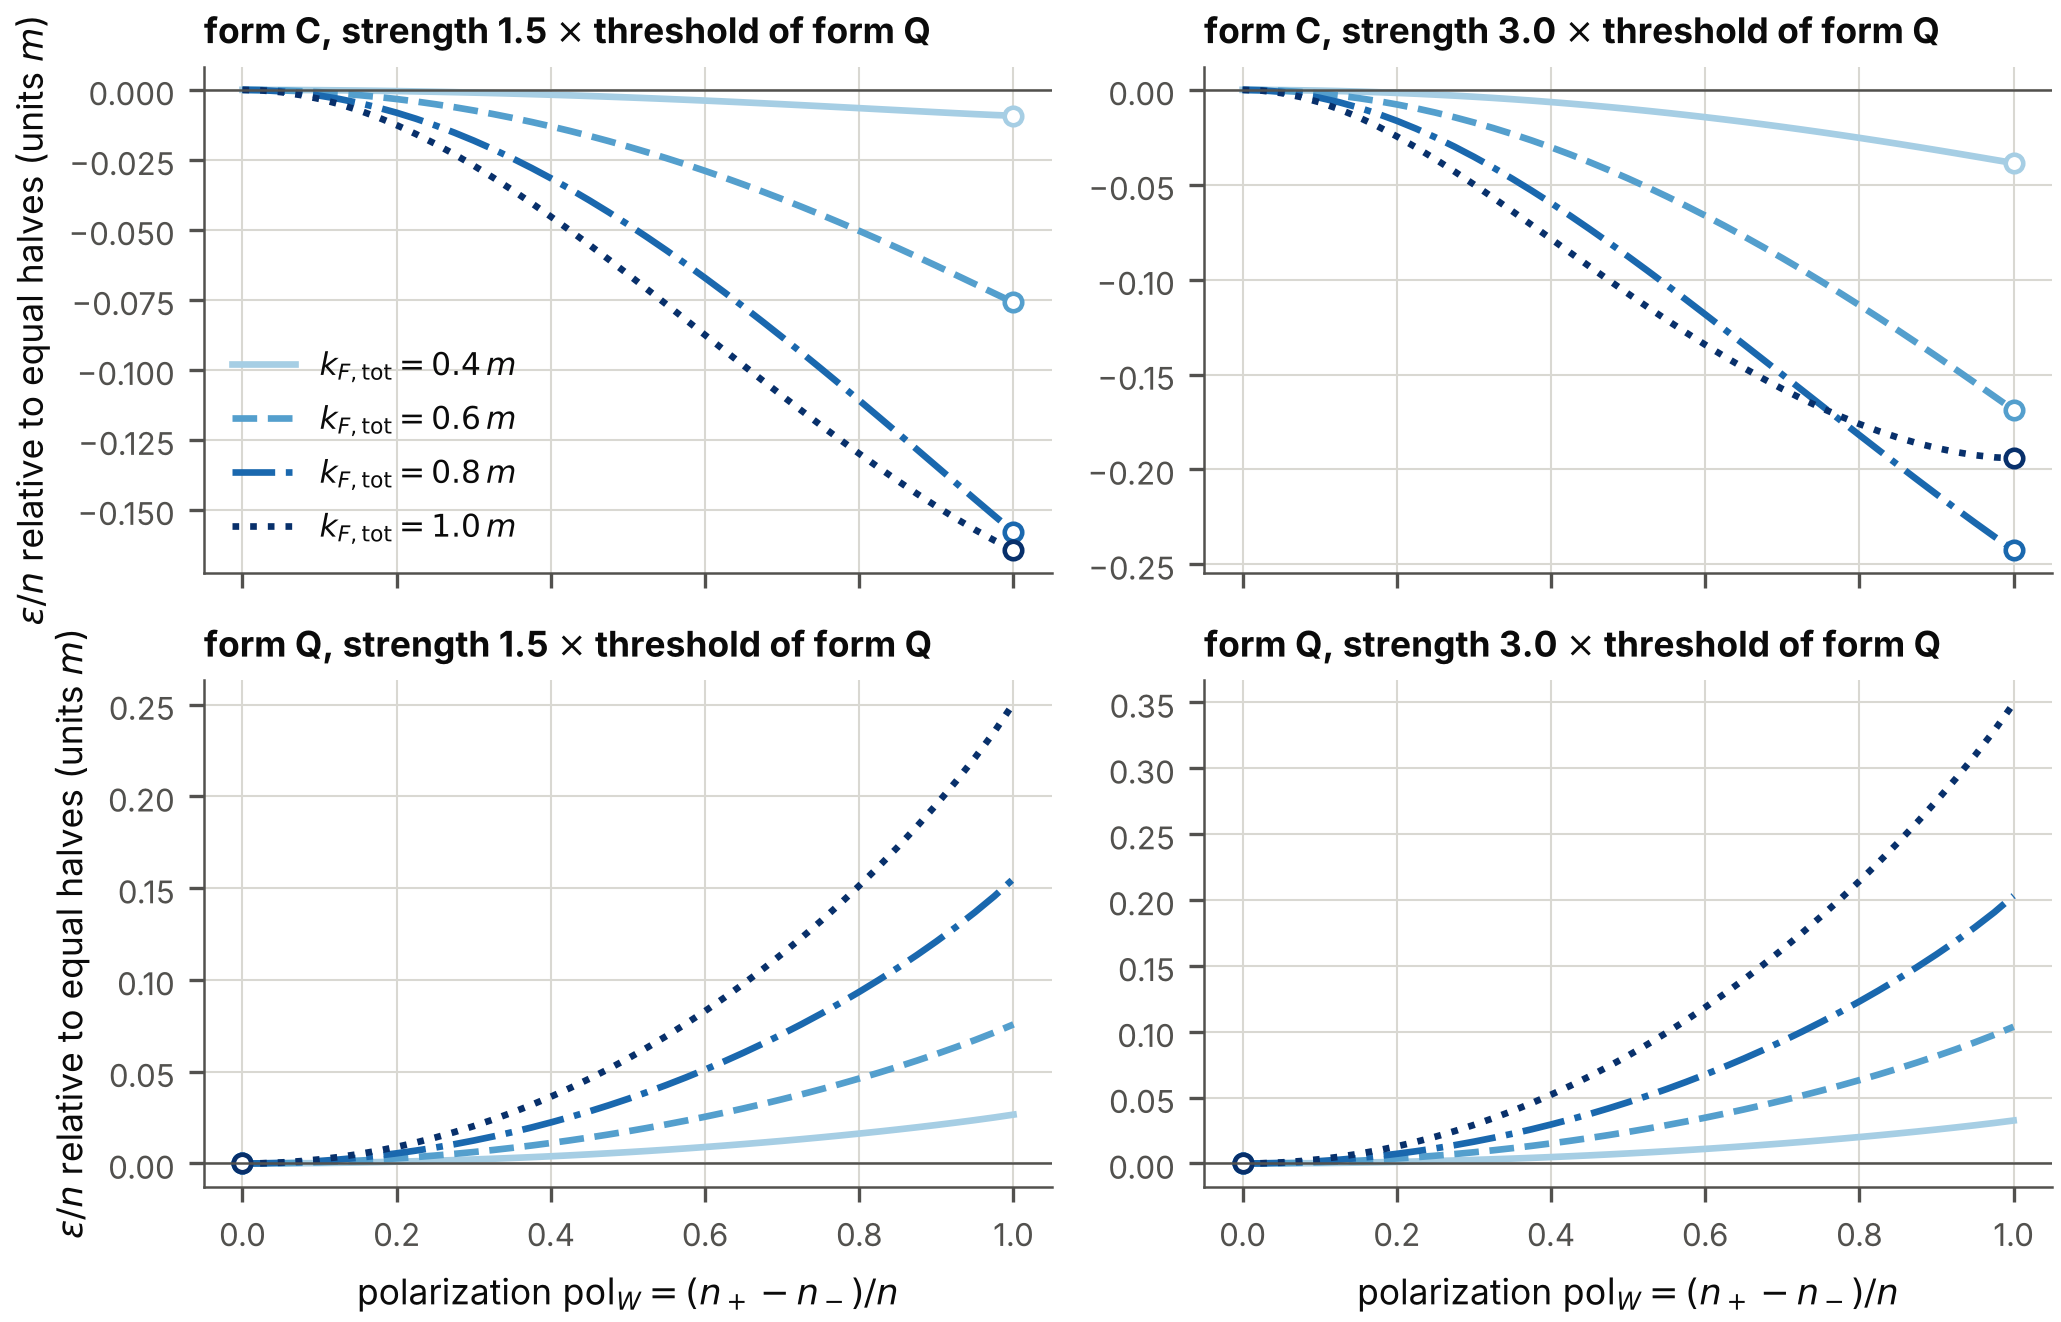
\includegraphics[width=0.96\textwidth,height=\textheight]{../figures/fig_forms_polarization.png}
\caption{Energy per particle of matter of a given total density against
the polarization of the two halves, relative to its value for equal
halves (\(D=4\), set A). Upper row: form C; lower row: form Q; left: 1.5
times, right: 3 times the strength at which form Q first binds matter.
The four curves are four total densities (light to dark and by line
style); the circle marks the lowest point of each curve. In form C the
lowest state has one half filled, or nearly so at the highest density;
in form Q it has equal halves.}
\end{figure}

In form C the energy falls with the polarization; in form Q it rises
(Figure 1). Over 48 cases (two dimensions, two sets, three strengths,
four densities) the state of lowest energy is polarized in 48 cases in
form C and in 0 cases in form Q (check \texttt{fm-F3}). The reason is
Eq. (5.5). For an attractive scalar coupling \(a_S<0\) and \(b_S<0\). In
form C a particle is attracted by the particles of its own half
(coupling \(a_S\)) and repelled by those of the other half (coupling
\(-b_S>0\)), so that the particles gather in one half. In form Q a
particle is attracted by both.

\emph{A limit of the calculation in form Q.} Of the 3936 states
examined, 108 states of form Q with unequal halves do not exist: at 3
and 6 times the threshold and at high density the attraction by the more
populated half, \(b_S\), which is stronger than the attraction \(a_S\)
inside a half, would make the mass of the particles of the less
populated half negative, and the gap equations have no solution with
non-negative masses. The states with equal halves and with one filled
half exist in all cases. In form C every state exists.

\hypertarget{the-strength-at-which-matter-first-binds}{%
\subsection{5.5 The strength at which matter first
binds}\label{the-strength-at-which-matter-first-binds}}

Matter is \textbf{self-bound} when its energy per particle, minimized
over the density and the polarization, lies below the mass \(m\). The
smallest strength \(g\) at which this happens is the binding threshold;
on the deflating spacetime it is reached at a definite clock reading.

\begin{longtable}[]{@{}
  >{\raggedleft\arraybackslash}p{(\columnwidth - 16\tabcolsep) * \real{0.0435}}
  >{\raggedright\arraybackslash}p{(\columnwidth - 16\tabcolsep) * \real{0.0580}}
  >{\raggedright\arraybackslash}p{(\columnwidth - 16\tabcolsep) * \real{0.0725}}
  >{\raggedleft\arraybackslash}p{(\columnwidth - 16\tabcolsep) * \real{0.1449}}
  >{\raggedright\arraybackslash}p{(\columnwidth - 16\tabcolsep) * \real{0.1884}}
  >{\raggedleft\arraybackslash}p{(\columnwidth - 16\tabcolsep) * \real{0.1304}}
  >{\raggedleft\arraybackslash}p{(\columnwidth - 16\tabcolsep) * \real{0.1159}}
  >{\raggedleft\arraybackslash}p{(\columnwidth - 16\tabcolsep) * \real{0.1159}}
  >{\raggedleft\arraybackslash}p{(\columnwidth - 16\tabcolsep) * \real{0.1304}}@{}}
\toprule\noalign{}
\begin{minipage}[b]{\linewidth}\raggedleft
\(D\)
\end{minipage} & \begin{minipage}[b]{\linewidth}\raggedright
set
\end{minipage} & \begin{minipage}[b]{\linewidth}\raggedright
form
\end{minipage} & \begin{minipage}[b]{\linewidth}\raggedleft
\(g\,m^{D-1}\)
\end{minipage} & \begin{minipage}[b]{\linewidth}\raggedright
state
\end{minipage} & \begin{minipage}[b]{\linewidth}\raggedleft
\(k_{F,\rm tot}/m\)
\end{minipage} & \begin{minipage}[b]{\linewidth}\raggedleft
\(M_+/m\)
\end{minipage} & \begin{minipage}[b]{\linewidth}\raggedleft
\(M_-/m\)
\end{minipage} & \begin{minipage}[b]{\linewidth}\raggedleft
\(\Lambda_{\max}/m\)
\end{minipage} \\
\midrule\noalign{}
\endhead
\bottomrule\noalign{}
\endlastfoot
4 & A & C & 224.7386 & one half & 0.6140 & 0.5239 & 1.5441 & 0.520 \\
4 & A & Q & 82.1116 & equal halves & 0.8054 & 0.4946 & 0.4946 & 0.727 \\
4 & B & C & 332.2917 & one half & 0.5211 & 0.5625 & 1.4842 & 0.449 \\
4 & B & Q & 121.0858 & equal halves & 0.6792 & 0.5424 & 0.5424 &
0.628 \\
3 & A & C & 24.5717 & one half & 0.5374 & 0.6454 & 1.4053 & 0.463 \\
3 & A & Q & 9.8090 & equal halves & 0.7356 & 0.6276 & 0.6276 & 0.733 \\
3 & B & C & 31.1674 & one half & 0.4635 & 0.6712 & 1.3638 & 0.400 \\
3 & B & Q & 12.3819 & equal halves & 0.6351 & 0.6575 & 0.6575 & 0.635 \\
\end{longtable}

(\(g\,m^{D-1}\) is the dimensionless strength; ``state'' is the state of
lowest energy just above the threshold; \(M_\pm\) are the masses of the
particles of the two halves, for an empty half the mass that a particle
of that half would have; \(\Lambda_{\max}\) is explained in Section 6.)
In form C the bound state has one half filled, in form Q equal halves,
in all eight cases (check \texttt{fm-F2}). Each threshold is verified
directly (bound 0.1 per cent above, not bound 0.1 per cent below) and
agrees with the threshold of matter of one kind of particle computed by
other routines, to \(5.7\times10^{-14}\): matter of form C with one
filled half is matter of \emph{one kind of particle with four internal
states and the couplings \(a_S\), \(a_V\)}; matter of form Q with equal
halves is matter of one kind with eight states and the couplings
\(T_S=G_S^{\rm HF}\), \(T_V=G_V^{\rm HF}\).

The ratio of the threshold of form C to that of form Q is 2.74 for set A
and 2.74 for set B in \(D=4\), and 2.51 and 2.52 in \(D=3\). On the
clock, form C binds matter later by \(\Delta\tau_d=\) 1.01 (set A) and
1.01 (set B) in \(D=4\), and by 0.92 and 0.92 in \(D=3\). Two things
make the difference. Only four of the eight internal states take part.
And the attraction inside one half, \(a_S=\tfrac78\,g_0\) for set A, is
weaker than the attraction between the halves, \(b_S=g_0\), from which
no exchange term is subtracted; matter of form Q with equal halves has
the benefit of both, \(T_S=\tfrac12(a_S+b_S)\).

\hypertarget{self-bound-matter-along-the-clock}{%
\subsection{5.6 Self-bound matter along the
clock}\label{self-bound-matter-along-the-clock}}

With the clock counted from the binding threshold of each case, so that
\(g=g_{\rm threshold}\,e^{\tau_d}\), the saturated state (the state of
lowest energy per particle) develops as follows. The table gives
\(\varepsilon/n-m\) in units of \(m\) at four clock readings, and, at
the clock readings 1 and 3, the mass \(M\) of the particles of the
filled half or halves and the Fermi momentum \(k=k_{F,\rm tot}\) that
the density would have with equal halves (both in units of \(m\)).

\begin{longtable}[]{@{}
  >{\raggedleft\arraybackslash}p{(\columnwidth - 20\tabcolsep) * \real{0.0357}}
  >{\raggedright\arraybackslash}p{(\columnwidth - 20\tabcolsep) * \real{0.0476}}
  >{\raggedright\arraybackslash}p{(\columnwidth - 20\tabcolsep) * \real{0.0595}}
  >{\raggedleft\arraybackslash}p{(\columnwidth - 20\tabcolsep) * \real{0.1190}}
  >{\raggedleft\arraybackslash}p{(\columnwidth - 20\tabcolsep) * \real{0.1190}}
  >{\raggedleft\arraybackslash}p{(\columnwidth - 20\tabcolsep) * \real{0.1190}}
  >{\raggedleft\arraybackslash}p{(\columnwidth - 20\tabcolsep) * \real{0.1190}}
  >{\raggedleft\arraybackslash}p{(\columnwidth - 20\tabcolsep) * \real{0.0952}}
  >{\raggedleft\arraybackslash}p{(\columnwidth - 20\tabcolsep) * \real{0.0952}}
  >{\raggedleft\arraybackslash}p{(\columnwidth - 20\tabcolsep) * \real{0.0952}}
  >{\raggedleft\arraybackslash}p{(\columnwidth - 20\tabcolsep) * \real{0.0952}}@{}}
\toprule\noalign{}
\begin{minipage}[b]{\linewidth}\raggedleft
\(D\)
\end{minipage} & \begin{minipage}[b]{\linewidth}\raggedright
set
\end{minipage} & \begin{minipage}[b]{\linewidth}\raggedright
form
\end{minipage} & \begin{minipage}[b]{\linewidth}\raggedleft
\(\tau_d=1\)
\end{minipage} & \begin{minipage}[b]{\linewidth}\raggedleft
\(2\)
\end{minipage} & \begin{minipage}[b]{\linewidth}\raggedleft
\(3\)
\end{minipage} & \begin{minipage}[b]{\linewidth}\raggedleft
\(4\)
\end{minipage} & \begin{minipage}[b]{\linewidth}\raggedleft
\(M\) at 1
\end{minipage} & \begin{minipage}[b]{\linewidth}\raggedleft
\(M\) at 3
\end{minipage} & \begin{minipage}[b]{\linewidth}\raggedleft
\(k\) at 1
\end{minipage} & \begin{minipage}[b]{\linewidth}\raggedleft
\(k\) at 3
\end{minipage} \\
\midrule\noalign{}
\endhead
\bottomrule\noalign{}
\endlastfoot
4 & A & C & \(-0.1092\) & \(-0.2079\) & \(-0.2913\) & \(-0.3597\) &
0.351 & 0.183 & 0.538 & 0.361 \\
4 & A & Q & \(-0.1284\) & \(-0.2449\) & \(-0.3438\) & \(-0.4254\) &
0.319 & 0.156 & 0.713 & 0.486 \\
4 & B & C & \(-0.0829\) & \(-0.1577\) & \(-0.2209\) & \(-0.2727\) &
0.392 & 0.215 & 0.452 & 0.301 \\
4 & B & Q & \(-0.0968\) & \(-0.1842\) & \(-0.2580\) & \(-0.3185\) &
0.371 & 0.199 & 0.592 & 0.395 \\
3 & A & C & \(-0.1226\) & \(-0.2400\) & \(-0.3365\) & \(-0.4116\) &
0.373 & 0.157 & 0.502 & 0.308 \\
3 & A & Q & \(-0.1424\) & \(-0.2801\) & \(-0.3945\) & \(-0.4844\) &
0.347 & 0.137 & 0.699 & 0.442 \\
3 & B & C & \(-0.0940\) & \(-0.1835\) & \(-0.2567\) & \(-0.3133\) &
0.407 & 0.183 & 0.426 & 0.256 \\
3 & B & Q & \(-0.1093\) & \(-0.2136\) & \(-0.2990\) & \(-0.3652\) &
0.389 & 0.170 & 0.588 & 0.357 \\
\end{longtable}

\begin{figure}
\centering
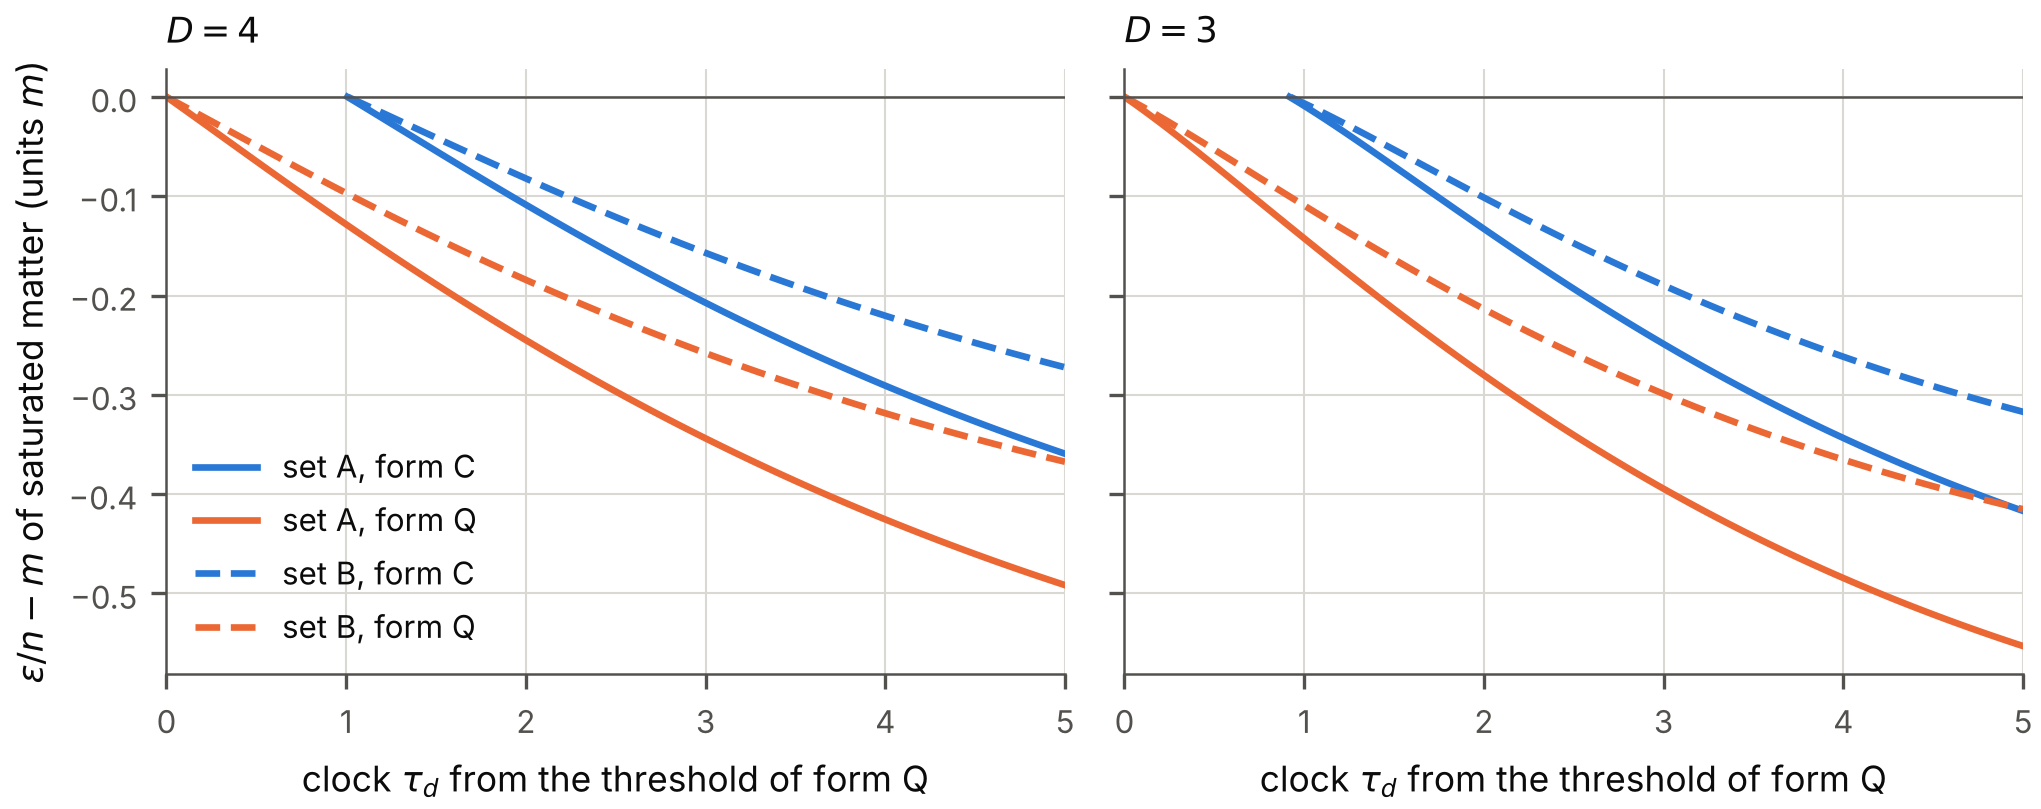
\includegraphics[width=0.96\textwidth,height=\textheight]{../figures/fig_forms_saturation.png}
\caption{Energy per particle minus the mass of self-bound (saturated)
matter along the deflation clock, for the same couplings of the
Lagrangian in both forms. The clock is counted here from the moment at
which form Q first binds matter of the same set, so that the curves of
form C begin later, where form C first binds. Solid lines: set A; dashed
lines: set B; blue: form C (one half filled); orange: form Q (equal
halves). Left: \(D=4\); right: \(D=3\).}
\end{figure}

Figure 2 shows the same development on one clock for both forms. At all
101 clock readings from 0 to 5 the kind of the state stays the same (one
half filled in form C, equal halves in form Q), the binding energy grows
monotonically, and the pressure vanishes (check \texttt{fm-F4}). Counted
from its own threshold, matter of form C is somewhat less strongly bound
than matter of form Q at the same clock reading. The largest eigenvalue
of the response matrix (5.13) along the table is 0.881: every state is
the regular continuation of the dilute gas. Beyond the table the
saturated state of form Q reaches the eigenvalue 1, at which its two
masses can split, at these clock readings: \(D=4\), set A:
\(\tau_d=6.416\); \(D=4\), set B: not before \(\tau_d=9\); \(D=3\), set
A: \(\tau_d=5.296\); \(D=3\), set B: \(\tau_d=7.323\). The saturated
state of form C has a negative eigenvalue throughout.

\hypertarget{matter-of-fixed-density-while-the-couplings-grow}{%
\subsection{5.7 Matter of fixed density while the couplings
grow}\label{matter-of-fixed-density-while-the-couplings-grow}}

A gas of a fixed number of particles per coordinate volume has a fixed
density of the weighted field while the couplings grow. The table gives
the clock readings, counted from the binding threshold of each case, at
which the two halves become unequal, at which one half is empty, and at
which the pressure \(p\) becomes negative (the matter is then under
tension and unstable against clumping). A dash means that the event does
not happen for \(-3\le\tau_d\le5\).

\begin{longtable}[]{@{}
  >{\raggedleft\arraybackslash}p{(\columnwidth - 12\tabcolsep) * \real{0.1429}}
  >{\raggedright\arraybackslash}p{(\columnwidth - 12\tabcolsep) * \real{0.1429}}
  >{\raggedright\arraybackslash}p{(\columnwidth - 12\tabcolsep) * \real{0.1429}}
  >{\raggedleft\arraybackslash}p{(\columnwidth - 12\tabcolsep) * \real{0.1429}}
  >{\raggedleft\arraybackslash}p{(\columnwidth - 12\tabcolsep) * \real{0.1429}}
  >{\raggedleft\arraybackslash}p{(\columnwidth - 12\tabcolsep) * \real{0.1429}}
  >{\raggedleft\arraybackslash}p{(\columnwidth - 12\tabcolsep) * \real{0.1429}}@{}}
\toprule\noalign{}
\begin{minipage}[b]{\linewidth}\raggedleft
\(D\)
\end{minipage} & \begin{minipage}[b]{\linewidth}\raggedright
set
\end{minipage} & \begin{minipage}[b]{\linewidth}\raggedright
form
\end{minipage} & \begin{minipage}[b]{\linewidth}\raggedleft
\(k_{F,\rm tot}/m\)
\end{minipage} & \begin{minipage}[b]{\linewidth}\raggedleft
halves unequal from
\end{minipage} & \begin{minipage}[b]{\linewidth}\raggedleft
one half empty from
\end{minipage} & \begin{minipage}[b]{\linewidth}\raggedleft
pressure negative from
\end{minipage} \\
\midrule\noalign{}
\endhead
\bottomrule\noalign{}
\endlastfoot
4 & A & C & 0.3 & \(-0.53\) & \(-0.17\) & \(+0.31\) \\
4 & A & C & 0.6 & \(-1.77\) & \(-1.43\) & \(-0.43\) \\
4 & A & Q & 0.3 & --- & --- & \(+0.78\) \\
4 & A & Q & 0.6 & --- & --- & \(-0.36\) \\
4 & B & C & 0.3 & \(-0.82\) & \(-0.47\) & \(+0.06\) \\
4 & B & C & 0.6 & \(-1.98\) & \(-1.62\) & --- \\
4 & B & Q & 0.3 & --- & --- & \(+0.51\) \\
4 & B & Q & 0.6 & --- & --- & \(-0.49\) \\
3 & A & C & 0.3 & \(-0.93\) & \(-0.72\) & \(-0.03\) \\
3 & A & C & 0.6 & \(-1.48\) & \(-1.27\) & --- \\
3 & A & Q & 0.3 & --- & --- & \(+0.21\) \\
3 & A & Q & 0.6 & --- & --- & \(-0.21\) \\
3 & B & C & 0.3 & \(-1.02\) & \(-0.88\) & \(-0.12\) \\
3 & B & C & 0.6 & \(-1.52\) & \(-1.32\) & --- \\
3 & B & Q & 0.3 & --- & --- & \(+0.10\) \\
3 & B & Q & 0.6 & --- & --- & \(-0.14\) \\
\end{longtable}

\begin{figure}
\centering
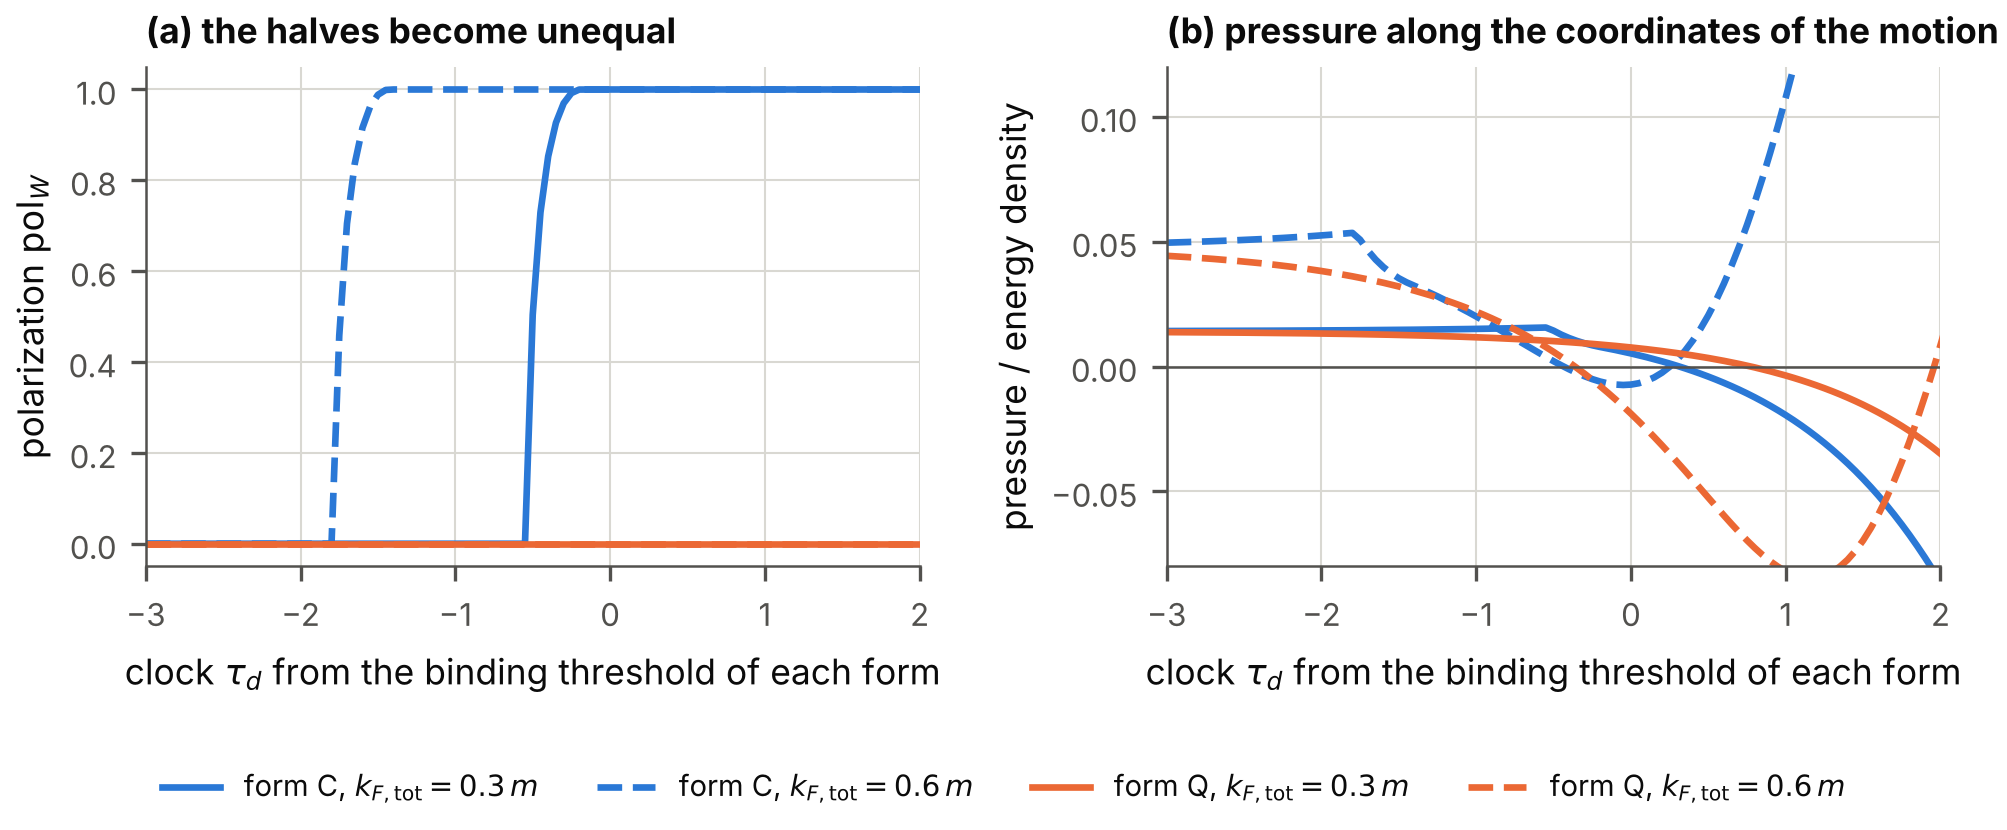
\includegraphics[width=0.96\textwidth,height=\textheight]{../figures/fig_forms_gas.png}
\caption{Matter of a fixed total density while the couplings grow
(\(D=4\), set A; the clock of each form is counted from its own binding
threshold). (a) The polarization: in form C the two halves become
unequal at a definite clock reading and one half empties soon after; in
form Q they stay equal. (b) The pressure along the coordinates of the
motion, divided by the energy density. Solid lines:
\(k_{F,\rm tot}=0.3\,m\); dashed lines: \(0.6\,m\).}
\end{figure}

In form C the gas polarizes before the binding threshold is reached
(Figure 3), within at most 0.35 of the clock from the first inequality
of the halves to an empty half. Where its pressure becomes negative,
that happens after the polarization; in 3 of the 8 cases (the higher
density) the pressure stays positive, because the repulsion \(a_V\)
between the particles of the filled half grows with the couplings while
the attraction saturates as the mass falls. In form Q the halves stay
equal and the pressure becomes negative in all cases (check
\texttt{fm-F5}).

\hypertarget{the-effective-potential-of-cornwall-jackiw-and-tomboulis-for-two-halves}{%
\subsection{5.8 The effective potential of Cornwall, Jackiw and
Tomboulis for two
halves}\label{the-effective-potential-of-cornwall-jackiw-and-tomboulis-for-two-halves}}

The same states follow from an effective potential (the CJT method in
the Hartree--Fock truncation). For two halves it is a function of the
two masses and the two energy shifts at a given chemical potential
\(\mu\),

\[\Omega(M_+,M_-,V_+,V_-;\mu)=\sum_\pm\Omega_1(M_\pm,\mu-V_\pm)-\frac{\mu_S^2}{2\,T_S}-\frac{d_S^2}{2\,D_S}-\frac{v_T^2}{2\,T_V}-\frac{v_D^2}{2\,D_V},\tag{5.14}\]

\[\mu_S=\tfrac12(M_++M_-)-m,\quad d_S=\tfrac12(M_+-M_-),\quad v_T=\tfrac12(V_++V_-),\quad v_D=\tfrac12(V_+-V_-),\tag{5.15}\]

where \(\Omega_1(M,\mu')=-4\int_{w<\mu'}d^Dk/(2\pi)^D\,(\mu'-w)\) is the
grand potential of free particles of the mass \(M\) with four internal
states. Its four stationarity conditions are the equations (5.7), and at
the stationary point \(-\Omega\) is the pressure and \(\Omega+\mu\,n\)
the energy density. For 80 states of both forms (40 with equal halves,
17 with unequal halves, 23 with one half filled) the stationary point of
\(\Omega\), found by Newton's method from displaced start values, agrees
with the Kohn--Sham state in both masses, density, energy density and
pressure to \(4.9\times10^{-11}\) (check \texttt{fm-F6}). The two
methods are equivalent in both forms.

\begin{center}\rule{0.5\linewidth}{0.5pt}\end{center}

\hypertarget{the-vacuum-with-the-filled-states-of-negative-energy}{%
\section{6. The vacuum with the filled states of negative
energy}\label{the-vacuum-with-the-filled-states-of-negative-energy}}

\hypertarget{the-gap-equations-of-the-vacuum}{%
\subsection{6.1 The gap equations of the
vacuum}\label{the-gap-equations-of-the-vacuum}}

When the states of negative energy are filled up to a cutoff \(\Lambda\)
of the momentum, the vacuum itself has scalar densities. The gap
equations (5.7) become

\[\tfrac12(M_++M_-)-m=T_S\,(s_++s_-),\qquad\tfrac12(M_+-M_-)=D_S\,(s_+-s_-),\qquad
s_\pm=-4\!\int_{|\mathbf k|<\Lambda}\!\frac{d^Dk}{(2\pi)^D}\,\frac{M_\pm}{w_\pm}.\tag{6.1}\]

The scalar density of the filled negative-energy states has the sign
opposite to the mass. For a field without mass term (\(m=0\)) the
solution \(M_+=M_-=0\) always exists. A second solution appears when the
more attractive of the two scalar couplings exceeds the \textbf{critical
coupling}

\[G_c=-\frac{(2\pi)^D\,(D-1)}{8\,A_D\,\Lambda^{D-1}},\tag{6.2}\]

with \(A_D\) the area of the unit sphere in \(D\) dimensions
(\(A_4=2\pi^2\), \(A_3=4\pi\)): \(G_c\Lambda^3=-3\pi^2\) for \(D=4\) and
\(G_c\Lambda^2=-\pi^2/2\) for \(D=3\).

\hypertarget{a-massless-field-acquires-the-mass-term-of-its-form}{%
\subsection{6.2 A massless field acquires the mass term of its
form}\label{a-massless-field-acquires-the-mass-term-of-its-form}}

For the sets A and B the attractive scalar coupling is
\(G_S^{\rm HF}<0\) in both forms, and the critical strength
\(g_{\rm crit}=G_c/(G_S^{\rm HF}/g)\) is the same for both. The table
gives it, and the masses of the two halves 2 per cent above it, in units
of the cutoff.

\begin{longtable}[]{@{}
  >{\raggedleft\arraybackslash}p{(\columnwidth - 10\tabcolsep) * \real{0.0476}}
  >{\raggedright\arraybackslash}p{(\columnwidth - 10\tabcolsep) * \real{0.0635}}
  >{\raggedleft\arraybackslash}p{(\columnwidth - 10\tabcolsep) * \real{0.1587}}
  >{\raggedleft\arraybackslash}p{(\columnwidth - 10\tabcolsep) * \real{0.1587}}
  >{\raggedleft\arraybackslash}p{(\columnwidth - 10\tabcolsep) * \real{0.2857}}
  >{\raggedleft\arraybackslash}p{(\columnwidth - 10\tabcolsep) * \real{0.2857}}@{}}
\toprule\noalign{}
\begin{minipage}[b]{\linewidth}\raggedleft
\(D\)
\end{minipage} & \begin{minipage}[b]{\linewidth}\raggedright
set
\end{minipage} & \begin{minipage}[b]{\linewidth}\raggedleft
\(G_c\Lambda^{D-1}\)
\end{minipage} & \begin{minipage}[b]{\linewidth}\raggedleft
\(g_{\rm crit}\Lambda^{D-1}\)
\end{minipage} & \begin{minipage}[b]{\linewidth}\raggedleft
form Q: \((M_+,M_-)/\Lambda\)
\end{minipage} & \begin{minipage}[b]{\linewidth}\raggedleft
form C: \((M_+,M_-)/\Lambda\)
\end{minipage} \\
\midrule\noalign{}
\endhead
\bottomrule\noalign{}
\endlastfoot
4 & A & \(-29.6088\) & 31.5827 & \((0.1243,\ 0.1243)\) &
\((0.1243,\ -0.1243)\) \\
4 & B & \(-29.6088\) & 29.9836 & \((0.1243,\ 0.1243)\) &
\((0.1243,\ -0.1243)\) \\
3 & A & \(-4.9348\) & 5.2638 & \((0.0860,\ 0.0860)\) &
\((0.0860,\ -0.0860)\) \\
3 & B & \(-4.9348\) & 4.9973 & \((0.0860,\ 0.0860)\) &
\((0.0860,\ -0.0860)\) \\
\end{longtable}

Below the critical strength the field stays massless in both forms.
Above it,

\begin{quote}
\textbf{in form Q the two halves acquire the same mass, \(M_+=M_-\): the
mass term \(-M\,\bar\psi\psi\) of the positive Lagrangian. In form C
they acquire masses of opposite sign, \(M_+=-M_-\): by Eq. (2.6) this is
the mass term \(-M\,\tilde\psi\psi\) of the covariant Lagrangian.}
\end{quote}

(Check \texttt{fm-F7}. The solutions of lowest \(\Omega\) are degenerate
by the exchange of the halves and, without mass term, by the reversal of
both signs; the table lists the representative with \(M_+>0\).) In form
C the attraction stands in \(D_S\), which couples to the
\emph{difference} of the scalar densities; a difference is what a mass
of opposite sign in the two halves produces. Each form generates
dynamically the mass term that belongs to its own adjoint. The magnitude
of the mass is the same in the two forms.

\hypertarget{with-a-bare-mass-a-crossover-in-form-q-a-transition-in-form-c}{%
\subsection{6.3 With a bare mass: a crossover in form Q, a transition in
form
C}\label{with-a-bare-mass-a-crossover-in-form-q-a-transition-in-form-c}}

The bare mass term of both forms is \(-m\,\bar\psi\psi\) (the positive
Lagrangian), the same for both halves. Along the clock, counted from the
critical strength of the massless field, the masses in vacuum develop as
follows (set A; in units of \(\Lambda\); a single number means
\(M_+=M_-\), a pair is \((M_+,M_-)\)):

\begin{longtable}[]{@{}
  >{\raggedleft\arraybackslash}p{(\columnwidth - 12\tabcolsep) * \real{0.0380}}
  >{\raggedleft\arraybackslash}p{(\columnwidth - 12\tabcolsep) * \real{0.1013}}
  >{\raggedright\arraybackslash}p{(\columnwidth - 12\tabcolsep) * \real{0.0633}}
  >{\raggedleft\arraybackslash}p{(\columnwidth - 12\tabcolsep) * \real{0.1139}}
  >{\raggedleft\arraybackslash}p{(\columnwidth - 12\tabcolsep) * \real{0.2278}}
  >{\raggedleft\arraybackslash}p{(\columnwidth - 12\tabcolsep) * \real{0.2278}}
  >{\raggedleft\arraybackslash}p{(\columnwidth - 12\tabcolsep) * \real{0.2278}}@{}}
\toprule\noalign{}
\begin{minipage}[b]{\linewidth}\raggedleft
\(D\)
\end{minipage} & \begin{minipage}[b]{\linewidth}\raggedleft
\(m_{\rm bare}/\Lambda\)
\end{minipage} & \begin{minipage}[b]{\linewidth}\raggedright
form
\end{minipage} & \begin{minipage}[b]{\linewidth}\raggedleft
\(\tau_d=-0.5\)
\end{minipage} & \begin{minipage}[b]{\linewidth}\raggedleft
\(0.1\)
\end{minipage} & \begin{minipage}[b]{\linewidth}\raggedleft
\(0.5\)
\end{minipage} & \begin{minipage}[b]{\linewidth}\raggedleft
\(1\)
\end{minipage} \\
\midrule\noalign{}
\endhead
\bottomrule\noalign{}
\endlastfoot
4 & 0 & Q & \(0\) & \(0.311\) & \(0.944\) & \(1.871\) \\
4 & 0 & C & \(0\) & \((0.311,\ -0.311)\) & \((0.944,\ -0.944)\) &
\((1.871,\ -1.871)\) \\
4 & 0.05 & Q & \(0.123\) & \(0.492\) & \(1.025\) & \(1.930\) \\
4 & 0.05 & C & \(0.048\) & \((0.350,\ -0.255)\) & \((0.992,\ -0.894)\) &
\((1.920,\ -1.821)\) \\
3 & 0 & Q & \(0\) & \(0.241\) & \(0.809\) & \(1.643\) \\
3 & 0 & C & \(0\) & \((0.241,\ -0.241)\) & \((0.809,\ -0.809)\) &
\((1.643,\ -1.643)\) \\
3 & 0.05 & Q & \(0.121\) & \(0.426\) & \(0.892\) & \(1.703\) \\
3 & 0.05 & C & \(0.048\) & \((0.278,\ -0.183)\) & \((0.855,\ -0.758)\) &
\((1.692,\ -1.593)\) \\
\end{longtable}

\begin{figure}
\centering
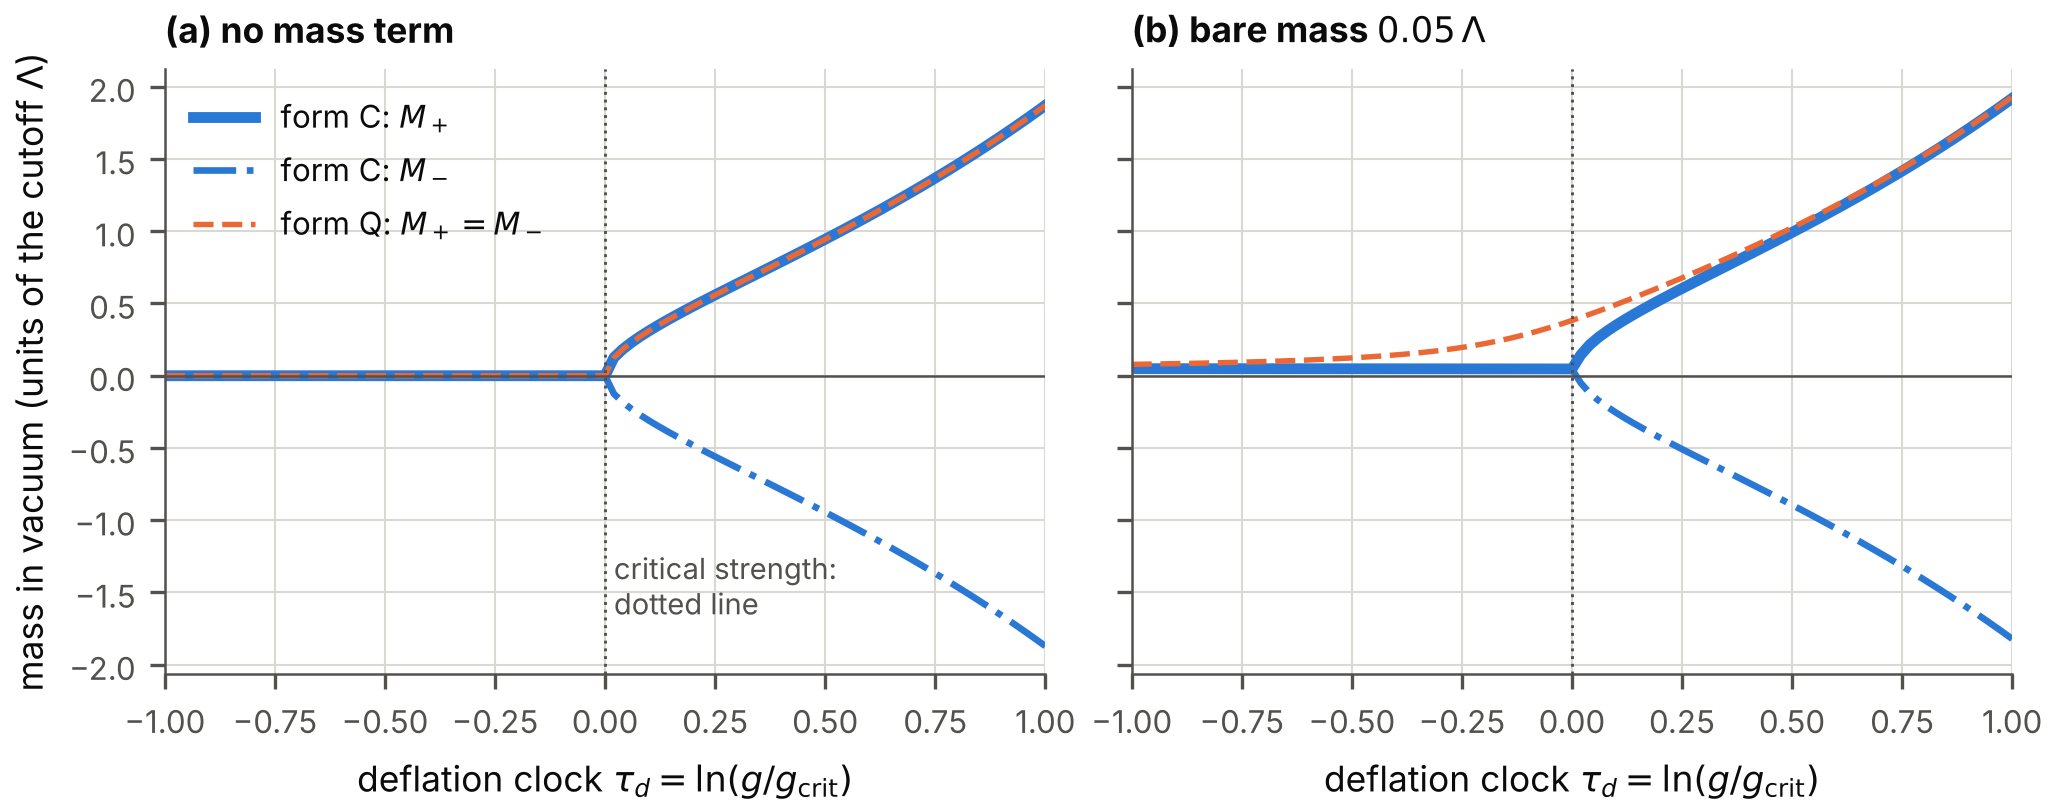
\includegraphics[width=0.96\textwidth,height=\textheight]{../figures/fig_forms_vacuum.png}
\caption{The masses of the particles of the two halves in vacuum with
the filled states of negative energy, along the clock counted from the
critical strength of a massless field (dotted line; \(D=4\), set A;
units of the cutoff). (a) A field without mass term: above the critical
strength form Q gives both halves the same mass, form C gives them
masses of opposite sign. (b) With the bare mass \(0.05\,\Lambda\): form
Q passes smoothly through the critical strength; in form C the two
masses are equal up to a sharp transition and separate there.}
\end{figure}

In form Q the bare mass and the dynamical mass have the same structure,
and the mass grows smoothly through the critical strength. In form C
they have different structures. Below a definite strength the two masses
are equal and slightly smaller than the bare mass (\(T_S>0\) repels the
total scalar density). At that strength the masses separate: there is a
sharp transition, at which the exchange symmetry of the two halves is
broken spontaneously. With the bare mass \(0.05\,\Lambda\) it lies at
\(D=4\), set A: \(\tau_d=0.009\); \(D=4\), set B: \(\tau_d=0.009\);
\(D=3\), set A: \(\tau_d=0.019\); \(D=3\), set B: \(\tau_d=0.020\), and
it agrees with the linear criterion
\(1+2\,D_S\cdot4\int^\Lambda d^Dk/(2\pi)^D\;k^2/w^3=0\) at the common
mass to \(2.1\times10^{-10}\) (check \texttt{fm-F7}).

\hypertarget{where-the-no-sea-approximation-of-section-5-applies}{%
\subsection{6.4 Where the no-sea approximation of Section 5
applies}\label{where-the-no-sea-approximation-of-section-5-applies}}

The matter of Section 5 was computed without the filled negative-energy
states. That is consistent only while the vacuum is stable, that is
while the most attractive scalar coupling stays below \(|G_c|\) of Eq.
(6.2) for the cutoff of the model. The column \(\Lambda_{\max}\) of the
table of thresholds gives, for each case, the largest cutoff (in units
of \(m\)) for which this holds \emph{at the binding threshold}. It is
below \(m\) in all eight cases, and smaller in form C than in form Q,
because form C needs stronger couplings to bind matter: \emph{in both
forms, and more so in form C, self-bound matter by contact couplings
alone lies outside the range in which the no-sea approximation is
controlled.} This limitation is the same as on the 7+1 spacetime; form C
does not remove it.

\begin{center}\rule{0.5\linewidth}{0.5pt}\end{center}

\hypertarget{pairs}{%
\section{7. Pairs}\label{pairs}}

\hypertarget{the-two-kinds-of-vector-pairs}{%
\subsection{7.1 The two kinds of vector
pairs}\label{the-two-kinds-of-vector-pairs}}

The superfluid of the project is a condensate of pairs. A pair of two
particles with the momenta \(\mathbf k\) and \(-\mathbf k\) is created
by an operator \(\psi^TX\psi\) with an antisymmetric matrix \(X\). The
seven \textbf{vector pairs} have \(X=C^-\gamma^A\) with \(A\neq4\): one
along each of the seven axes other than the ordinary time. The pair
along the hidden axis, \(X=C^-\gamma^0\), is the spin-singlet pair that
the project studies; it and the three pairs along \(x5,x6,x7\) are
scalars under the rotations of ordinary space, and the pairs along
\(x1,x2,x3\) form a vector of ordinary space.

The pair density \(\kappa_{ab}=\langle\psi_a\psi_b\rangle\) of a vector
pair has a definite behavior under \(W\) (check \texttt{44c-S9}):

\[\begin{aligned}
W\,\kappa\,W^T&=-\kappa\quad\text{for the pairs along }x0,x1,x2,x3,\\
W\,\kappa\,W^T&=+\kappa\quad\text{for the pairs along }x5,x6,x7.
\end{aligned}\tag{7.1}\]

A pair along one of the four space-like axes consists of \textbf{one
particle of each half}; a pair along one of the three extra time-like
axes consists of \textbf{two particles of the same half}. By Section 4.2
the two forms therefore agree on the pairs along \(x5,x6,x7\) and have
opposite signs on the pairs along \(x0,\dots,x3\).

\hypertarget{two-particles-at-rest}{%
\subsection{7.2 Two particles at rest}\label{two-particles-at-rest}}

Two particles at rest, with eight internal states each, form
\(8\cdot7/2=28\) antisymmetric states. Each is an eigenstate of the
interaction, with the eigenvalue \(G_{\rm pair}\) (the interaction
energy of the pair times the volume; attractive if negative). In exact
arithmetic (checks \texttt{44c-S9}, \texttt{44q-S9}):

\begin{longtable}[]{@{}
  >{\raggedright\arraybackslash}p{(\columnwidth - 6\tabcolsep) * \real{0.2500}}
  >{\raggedleft\arraybackslash}p{(\columnwidth - 6\tabcolsep) * \real{0.2500}}
  >{\raggedright\arraybackslash}p{(\columnwidth - 6\tabcolsep) * \real{0.2500}}
  >{\raggedright\arraybackslash}p{(\columnwidth - 6\tabcolsep) * \real{0.2500}}@{}}
\toprule\noalign{}
\begin{minipage}[b]{\linewidth}\raggedright
form
\end{minipage} & \begin{minipage}[b]{\linewidth}\raggedleft
number of pairs
\end{minipage} & \begin{minipage}[b]{\linewidth}\raggedright
the two particles are in
\end{minipage} & \begin{minipage}[b]{\linewidth}\raggedright
\(G_{\rm pair}\)
\end{minipage} \\
\midrule\noalign{}
\endhead
\bottomrule\noalign{}
\endlastfoot
C & 4 & different halves &
\(-g_0^{\rm eff}-g_1^{\rm eff}-5\,g_7^{\rm eff}\) \\
C & 12 & different halves &
\(-g_0^{\rm eff}-g_1^{\rm eff}+3\,g_7^{\rm eff}\) \\
C & 9 & same half & \(g_0^{\rm eff}+g_1^{\rm eff}-3\,g_7^{\rm eff}\) \\
C & 3 & same half & \(g_0^{\rm eff}+g_1^{\rm eff}+5\,g_7^{\rm eff}\) \\
Q & 12 & different halves &
\(g_0^{\rm eff}+g_1^{\rm eff}-3\,g_7^{\rm eff}\) \\
Q & 4 & different halves &
\(g_0^{\rm eff}+g_1^{\rm eff}+5\,g_7^{\rm eff}\) \\
Q & 9 & same half & \(g_0^{\rm eff}+g_1^{\rm eff}-3\,g_7^{\rm eff}\) \\
Q & 3 & same half & \(g_0^{\rm eff}+g_1^{\rm eff}+5\,g_7^{\rm eff}\) \\
\end{longtable}

In form Q the seven vector pairs are degenerate, with
\(G_{\rm pair}=g_0^{\rm eff}+g_1^{\rm eff}+5\,g_7^{\rm eff}\). In form C
they split into the four pairs along the space-like axes, with
\(-(g_0^{\rm eff}+g_1^{\rm eff}+5\,g_7^{\rm eff})\), and the three pairs
along the extra axes, with
\(+(g_0^{\rm eff}+g_1^{\rm eff}+5\,g_7^{\rm eff})\). \emph{A scalar
coupling that attracts in form Q repels in the hidden-axis pair of form
C.}

\hypertarget{pairs-with-momentum-the-amplitudes}{%
\subsection{7.3 Pairs with momentum: the
amplitudes}\label{pairs-with-momentum-the-amplitudes}}

For particles of mass \(M\) with the momenta
\(\mathbf p,-\mathbf p\to\mathbf p',-\mathbf p'\) in ordinary space and
the energies \(E,E'\), the amplitudes of the four independent contact
channels in the pair along the hidden axis and in the pairs along
\(x5,x6,x7\) (the four pairs whose axis is perpendicular to ordinary
space) are, in form Q and on 7+1,

\[\begin{aligned}
F_0&=\frac{EE'+M^2-\mathbf p\cdot\mathbf p'}{2\,EE'},&\qquad F_8&=-\frac{EE'-M^2-\mathbf p\cdot\mathbf p'}{2\,EE'},\\
F_1&=\frac{3\,EE'-2M^2-\mathbf p\cdot\mathbf p'}{EE'},&\qquad F_7&=\frac{3\,EE'+2M^2-\mathbf p\cdot\mathbf p'}{EE'},
\end{aligned}\tag{7.2}\]

and the pairing potential of the contact interaction is

\[V_{\rm contact}=s\,\big(g_0^{\rm eff}F_0+g_1^{\rm eff}F_1+g_7^{\rm eff}F_7+g_8^{\rm eff}F_8\big),\tag{7.3}\]

attractive where negative, with the sign

\[\begin{aligned}
s&=+1:\quad\text{form Q, all four pairs; form C, the pairs along }x5,x6,x7;\\
s&=-1:\quad\text{form C, the pair along the hidden axis }x0.
\end{aligned}\tag{7.4}\]

This holds at all momenta, verified by direct evaluation with the 256
matrices of each form and the projectors on the states of positive
energy (check \texttt{pc-P5}), and independently with projectors built
from numerical eigenvectors (check \texttt{Icks-F3}). At rest
\((F_0,F_1,F_7,F_8)=(1,1,5,0)\), which is Section 7.2.

\hypertarget{the-exchange-of-the-vorton-scalar-is-not-affected}{%
\subsection{7.4 The exchange of the Vorton-Scalar is not
affected}\label{the-exchange-of-the-vorton-scalar-is-not-affected}}

The complex scalar field of the project (the Vorton-Scalar, with the
coupling \(g_{VS}\)) couples to the fermions through \(\bar\psi\psi\)
and \(\bar\psi\,i\chi\,\psi\), with the adjoint
\(\bar\psi=\psi^\dagger\beta\) in both forms (Section 9). The exchange
of its radial mode (mass \(m_s\)) and of its phase mode (mass
\(m_\vartheta\)) gives the pairing potential

\[V_{VS}=-g_{VS}^2\left[\frac{F_S}{q^2+m_s^2}+\frac{F_P}{q^2+m_\vartheta^2}\right],\qquad
F_S=F_0,\quad F_P=-F_8,\quad\mathbf q=\mathbf p'-\mathbf p,\tag{7.5}\]

in each of these four pairs and in both forms: the two halves enter
\(\bar\psi\psi\) alike. \emph{In form C the contact self-interaction
therefore distinguishes the pair along the hidden axis from the pairs
along \(x5,x6,x7\), and the exchange does not.}

\hypertarget{the-gap}{%
\subsection{7.5 The gap}\label{the-gap}}

The gap \(\Delta\) at the Fermi surface follows from the gap equation

\[\Delta(k)=\frac1{4\pi^2}\int_0^{K}dk'\,k'^2\;\mathsf W(k,k')\,\frac{\Delta(k')}{\sqrt{\xi(k')^2+\Delta(k')^2}},\qquad
\mathsf W(k,k')=\frac12\int_{-1}^{1}d\cos\theta\,\big[-V\big],\tag{7.6}\]

with \(\xi=\sqrt{k^2+M^2}-\sqrt{k_F^2+M^2}\), the potential
\(V=V_{VS}+V_{\rm contact}\), the angle \(\theta\) between \(\mathbf k\)
and \(\mathbf k'\), and an upper limit \(K\) of the momentum integral
(Section 7.6). Each contact coupling is given the range \(1/m_{\rm ct}\)
of an exchanged heavy particle,
\(g\to g\,m_{\rm ct}^2/(q^2+m_{\rm ct}^2)\), with \(m_{\rm ct}=m\) in
the numbers below. All couplings grow as \(e^{\tau_d}\):
\(g_{VS}=e^{\tau_d/2}\), and the contact couplings are given in units of
\(g_{VS}^2/m^2\). The table gives the gap in units of the Fermi kinetic
energy at the clock reading 2.04, for \(k_F=0.5\,m\) and two masses of
the radial mode, for the two signs \(s\) of Eq. (7.4), together with the
ultraviolet strength of Section 7.6 (for \(m_s=m\)).

\begin{longtable}[]{@{}
  >{\raggedright\arraybackslash}p{(\columnwidth - 12\tabcolsep) * \real{0.3864}}
  >{\raggedleft\arraybackslash}p{(\columnwidth - 12\tabcolsep) * \real{0.1136}}
  >{\raggedleft\arraybackslash}p{(\columnwidth - 12\tabcolsep) * \real{0.0909}}
  >{\raggedleft\arraybackslash}p{(\columnwidth - 12\tabcolsep) * \real{0.1136}}
  >{\raggedleft\arraybackslash}p{(\columnwidth - 12\tabcolsep) * \real{0.0909}}
  >{\raggedleft\arraybackslash}p{(\columnwidth - 12\tabcolsep) * \real{0.1136}}
  >{\raggedleft\arraybackslash}p{(\columnwidth - 12\tabcolsep) * \real{0.0909}}@{}}
\toprule\noalign{}
\begin{minipage}[b]{\linewidth}\raggedright
interaction
\end{minipage} & \begin{minipage}[b]{\linewidth}\raggedleft
\(m_s=0.3m\), \(s=+1\)
\end{minipage} & \begin{minipage}[b]{\linewidth}\raggedleft
\(s=-1\)
\end{minipage} & \begin{minipage}[b]{\linewidth}\raggedleft
\(m_s=m\), \(s=+1\)
\end{minipage} & \begin{minipage}[b]{\linewidth}\raggedleft
\(s=-1\)
\end{minipage} & \begin{minipage}[b]{\linewidth}\raggedleft
\(U/4\pi^2\), \(s=+1\)
\end{minipage} & \begin{minipage}[b]{\linewidth}\raggedleft
\(s=-1\)
\end{minipage} \\
\midrule\noalign{}
\endhead
\bottomrule\noalign{}
\endlastfoot
exchange of the Vorton-Scalar alone & 0.4118 & 0.4118 & 0.0247 & 0.0247
& 0.285 & 0.285 \\
with \(g_0^{\rm eff}=-g_{VS}^2/m^2\) & 0.9035 & 0.1481 & 0.2975 & 0.0000
& 0.428 & 0.143 \\
with \(g_0^{\rm eff}=-g_{VS}^2/m^2\),
\(g_1^{\rm eff}=+0.1\,g_{VS}^2/m^2\) & 0.7407 & 0.1875 & 0.1963 & 0.0000
& 0.304 & 0.267 \\
with \(g_1^{\rm eff}=+0.3\,g_{VS}^2/m^2\) & 0.2370 & 0.8481 & 0.0006 &
0.2285 & -0.088 & 0.659 \\
with \(g_7^{\rm eff}=-0.1\,g_{VS}^2/m^2\) & 0.6459 & 0.2509 & 0.1290 &
0.0007 & 0.410 & 0.161 \\
contact couplings alone (\(g_0^{\rm eff}=-g_{VS}^2/m^2\),
\(g_1^{\rm eff}=+0.1\,g_{VS}^2/m^2\)) & 0.0006 & 0.0000 & 0.0006 &
0.0000 & 0.018 & -0.018 \\
\end{longtable}

\begin{figure}
\centering
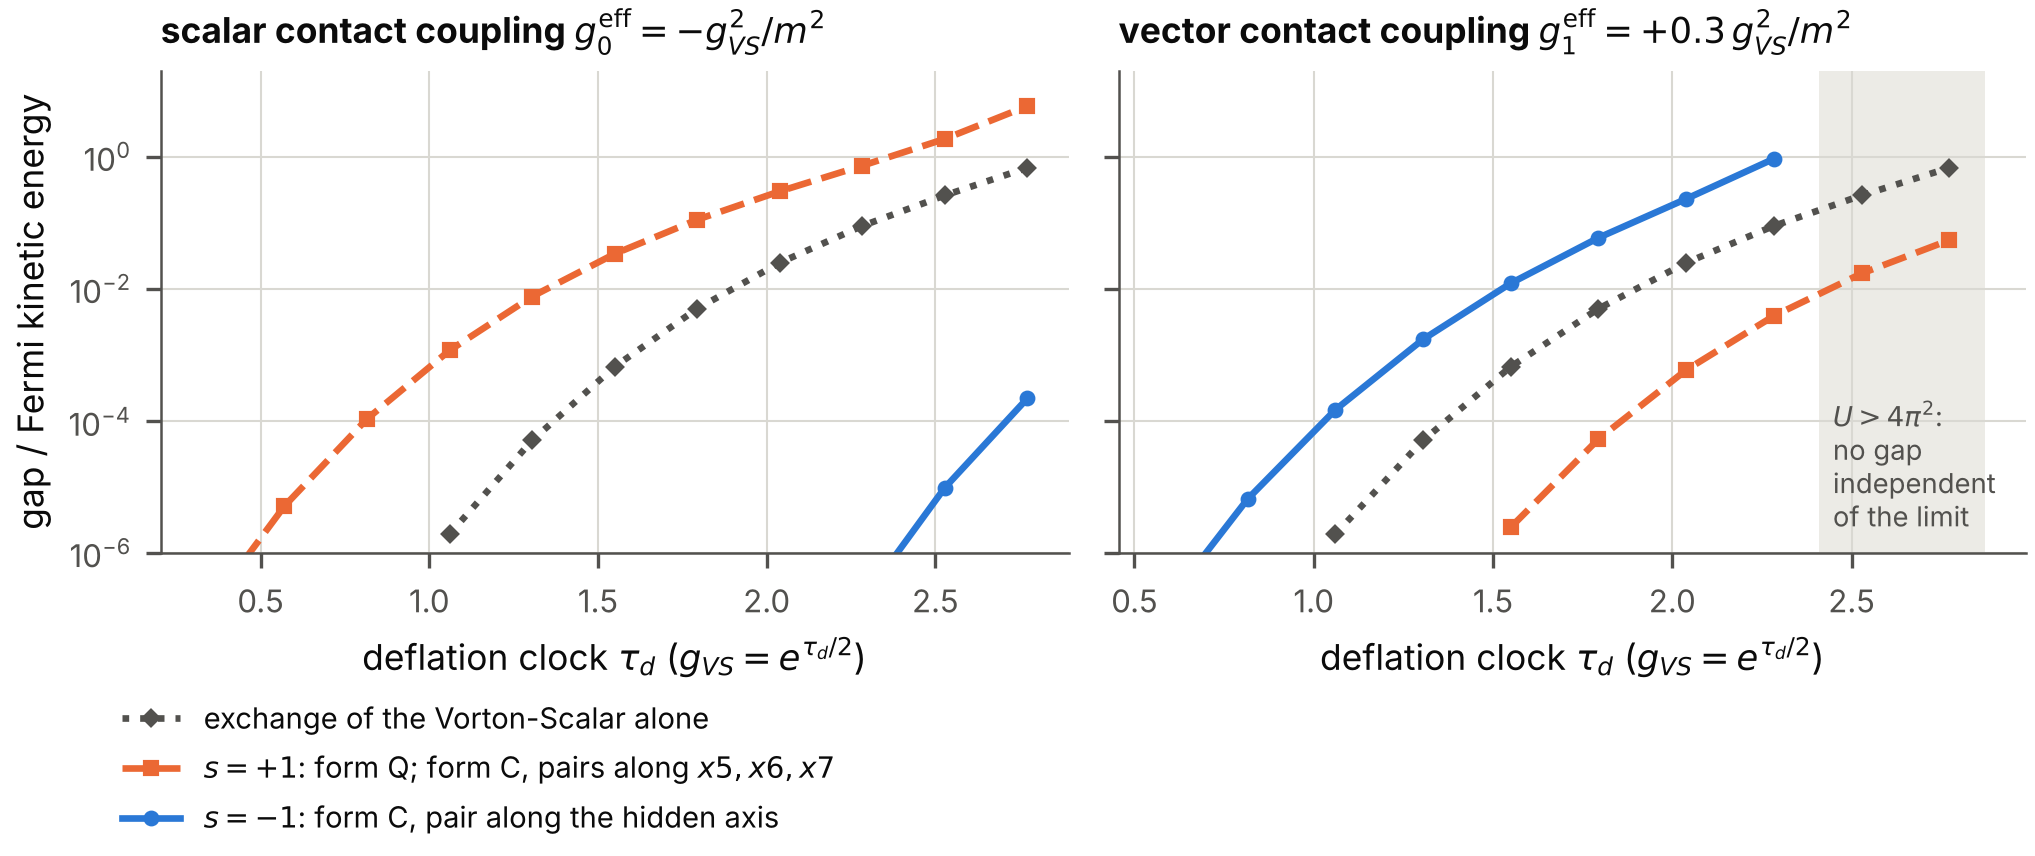
\includegraphics[width=0.96\textwidth,height=\textheight]{../figures/fig_forms_gap.png}
\caption{The gap at the Fermi surface, in units of the Fermi kinetic
energy, along the deflation clock, for \(m_s=m\) and \(k_F=0.5\,m\).
Left: with the scalar contact coupling \(g_0^{\rm eff}=-g_{VS}^2/m^2\);
right: with the vector contact coupling
\(g_1^{\rm eff}=+0.3\,g_{VS}^2/m^2\). Dotted line: the exchange of the
Vorton-Scalar alone. Dashed line (squares): the contact coupling with
the sign \(s=+1\) (form Q; form C in the pairs along \(x5,x6,x7\)).
Solid line (circles): with the sign \(s=-1\) (form C in the pair along
the hidden axis). In the shaded band the kernel with \(s=-1\) exceeds
the ultraviolet criterion of Section 7.6, and no gap is given.}
\end{figure}

With \(s=+1\) a scalar contact attraction raises the gap and a vector
contact repulsion lowers it (Figure 5). With \(s=-1\) (the hidden-axis
pair of form C) the same couplings act in the opposite way: the scalar
coupling lowers the gap (for \(m_s=m\) it removes it at this clock
reading), and the vector coupling raises it (checks \texttt{pc-P4},
\texttt{pc-P6}; the gap with \(s=-1\) and the vector coupling agrees
with an independent solution of the gap equation to
\(7.8\times10^{-5}\)). Which of the two kinds of pairs has the larger
gap, over the clock readings at which both gaps are defined:

\begin{longtable}[]{@{}
  >{\raggedright\arraybackslash}p{(\columnwidth - 4\tabcolsep) * \real{0.3333}}
  >{\raggedleft\arraybackslash}p{(\columnwidth - 4\tabcolsep) * \real{0.3333}}
  >{\raggedleft\arraybackslash}p{(\columnwidth - 4\tabcolsep) * \real{0.3333}}@{}}
\toprule\noalign{}
\begin{minipage}[b]{\linewidth}\raggedright
interaction
\end{minipage} & \begin{minipage}[b]{\linewidth}\raggedleft
readings at which the pairs along \(x5,x6,x7\) have the larger gap
\end{minipage} & \begin{minipage}[b]{\linewidth}\raggedleft
readings at which the hidden-axis pair has
\end{minipage} \\
\midrule\noalign{}
\endhead
\bottomrule\noalign{}
\endlastfoot
with \(g_0^{\rm eff}=-g_{VS}^2/m^2\) & 53 & 0 \\
with \(g_0^{\rm eff}=-g_{VS}^2/m^2\),
\(g_1^{\rm eff}=+0.1\,g_{VS}^2/m^2\) & 53 & 0 \\
with \(g_1^{\rm eff}=+0.3\,g_{VS}^2/m^2\) & 0 & 43 \\
with \(g_7^{\rm eff}=-0.1\,g_{VS}^2/m^2\) & 51 & 0 \\
\end{longtable}

\begin{quote}
\textbf{In form C the self-interaction removes the degeneracy of the
pair along the hidden axis with the pairs along \(x5,x6,x7\), and so
selects the direction of the order parameter.} With an attractive scalar
coupling the pairs along the extra time-like axes \(x5,x6,x7\) have the
larger gap, not the pair along the hidden axis. With a repulsive vector
coupling alone the pair along the hidden axis has the larger gap. In
form Q, as on 7+1, the four pairs have the same gap, and the direction
is free.
\end{quote}

\hypertarget{the-ultraviolet-criterion-of-the-gap-equation}{%
\subsection{7.6 The ultraviolet criterion of the gap
equation}\label{the-ultraviolet-criterion-of-the-gap-equation}}

At momenta far above all masses every term of the pairing potential has
the form (coupling) \(\times\) (function of \(\cos\theta\)) \(/q^2\),
with \(F_0,F_S,F_P\to\tfrac12(1-\cos\theta)\),
\(F_8\to-\tfrac12(1-\cos\theta)\) and \(F_1,F_7\to3-\cos\theta\). The
kernel is then homogeneous, \(\mathsf W(k,k')\to\mathsf w(k'/k)/k^2\),
and above the gap Eq. (7.6) reads
\(\Delta(k)=\tfrac1{4\pi^2}\int_0^\infty dt\,t\,\mathsf w(t)\,\Delta(tk)\).
A power \(\Delta\propto k^{-\mathsf s}\) solves it if

\[J(\mathsf s)\equiv\int_0^\infty dt\;t^{1-\mathsf s}\,\mathsf w(t)=4\pi^2.\tag{7.7}\]

Because \(\mathsf W\) is symmetric in its arguments,
\(\mathsf w(1/t)=t^2\,\mathsf w(t)\) and
\(J(2-\mathsf s)=J(\mathsf s)\): the two exponents are
\(\mathsf s=1\pm\sigma\), and \(J\) is smallest at \(\mathsf s=1\).
Define the \textbf{ultraviolet strength}

\[U=J(1)=\int_0^\infty dt\;\mathsf w(t).\tag{7.8}\]

\begin{itemize}
\tightlist
\item
  If \(U<4\pi^2\) the exponents are real, the gap function falls as
  \(k^{-1-\sigma}\), and the gap equation has a solution that does not
  depend on the upper limit \(K\); it is approached as \(K^{-2\sigma}\),
  slowly when \(U\) is close to \(4\pi^2\).
\item
  If \(U>4\pi^2\) the exponents are complex, no such solution exists,
  and with an upper limit the gap grows in proportion to \(K\): the pair
  collapses to short distances. This is the fall to the center of
  relativistic particles in a potential \(-\alpha/r\) with \(\alpha\)
  above its critical value. The Fourier transform of \(g/(q^2+\mu^2)\)
  is the Yukawa potential \(g\,e^{-\mu r}/(4\pi r)\), which is a Coulomb
  potential at distances below \(1/\mu\).
\end{itemize}

The integral of one term is elementary. With
\(\int_0^\infty dt/(1+t^2-2t\cos\theta)=(\pi-\theta)/\sin\theta\),

\[\int_0^\infty dt\;\frac12\int_{-1}^{1}dx\,\frac{a+b\,x}{1+t^2-2tx}=\frac{\pi^2}{4}\,a+b,\tag{7.9}\]

that is \(I_S=\pi^2/8-\tfrac12=\) 0.7337 for \(\tfrac12(1-x)\) and
\(I_V=3\pi^2/4-1=\) 6.4022 for \(3-x\). Therefore

\[\boxed{\ U=g_{VS}^2\Big(\frac{\pi^2}{4}-1\Big)-s\,m_{\rm ct}^2\Big[\big(g_0^{\rm eff}-g_8^{\rm eff}\big)\Big(\frac{\pi^2}{8}-\frac12\Big)+\big(g_1^{\rm eff}+g_7^{\rm eff}\big)\Big(\frac{3\pi^2}{4}-1\Big)\Big]\ }\tag{7.10}\]

when both modes of the Vorton-Scalar are exchanged (half the first term
for the radial mode alone). The formula is verified against the
numerical integral of the kernel (unit test of the program; check
\texttt{Icks-F8} of the independent script). Per unit \(g_{VS}^2\), with
the contact couplings of the table of Section 7.5:

\begin{longtable}[]{@{}
  >{\raggedright\arraybackslash}p{(\columnwidth - 12\tabcolsep) * \real{0.4048}}
  >{\raggedleft\arraybackslash}p{(\columnwidth - 12\tabcolsep) * \real{0.1190}}
  >{\raggedleft\arraybackslash}p{(\columnwidth - 12\tabcolsep) * \real{0.1071}}
  >{\raggedleft\arraybackslash}p{(\columnwidth - 12\tabcolsep) * \real{0.0714}}
  >{\raggedleft\arraybackslash}p{(\columnwidth - 12\tabcolsep) * \real{0.1190}}
  >{\raggedleft\arraybackslash}p{(\columnwidth - 12\tabcolsep) * \real{0.1071}}
  >{\raggedleft\arraybackslash}p{(\columnwidth - 12\tabcolsep) * \real{0.0714}}@{}}
\toprule\noalign{}
\begin{minipage}[b]{\linewidth}\raggedright
interaction
\end{minipage} & \begin{minipage}[b]{\linewidth}\raggedleft
\(s=+1\): \(U/g_{VS}^2\)
\end{minipage} & \begin{minipage}[b]{\linewidth}\raggedleft
critical \(g_{VS}^2\)
\end{minipage} & \begin{minipage}[b]{\linewidth}\raggedleft
\(\tau_d\)
\end{minipage} & \begin{minipage}[b]{\linewidth}\raggedleft
\(s=-1\): \(U/g_{VS}^2\)
\end{minipage} & \begin{minipage}[b]{\linewidth}\raggedleft
critical \(g_{VS}^2\)
\end{minipage} & \begin{minipage}[b]{\linewidth}\raggedleft
\(\tau_d\)
\end{minipage} \\
\midrule\noalign{}
\endhead
\bottomrule\noalign{}
\endlastfoot
exchange of the Vorton-Scalar alone & 1.467 & 26.90 & 3.29 & 1.467 &
26.90 & 3.29 \\
with \(g_0^{\rm eff}=-g_{VS}^2/m^2\) & 2.201 & 17.94 & 2.89 & 0.734 &
53.81 & 3.99 \\
with \(g_0^{\rm eff}=-g_{VS}^2/m^2\),
\(g_1^{\rm eff}=+0.1\,g_{VS}^2/m^2\) & 1.561 & 25.29 & 3.23 & 1.374 &
28.73 & 3.36 \\
with \(g_1^{\rm eff}=+0.3\,g_{VS}^2/m^2\) & \(-0.453\) & --- & --- &
3.388 & 11.65 & 2.46 \\
with \(g_7^{\rm eff}=-0.1\,g_{VS}^2/m^2\) & 2.108 & 18.73 & 2.93 & 0.827
& 47.73 & 3.87 \\
contact couplings alone (\(g_0^{\rm eff}=-g_{VS}^2/m^2\),
\(g_1^{\rm eff}=+0.1\,g_{VS}^2/m^2\)) & 0.093 & 422.32 & 6.05 &
\(-0.093\) & --- & --- \\
\end{longtable}

The exchange of the two modes alone reaches \(U=4\pi^2\) at
\(g_{VS}^2=4\pi^2/(\pi^2/4-1)=\) 26.90, the clock reading 3.29, beyond
the last reading 2.77 of the gap histories of this folder. The vector
contact coupling \(+0.3\,g_{VS}^2/m^2\) in the hidden-axis pair of form
C reaches it at \(g_{VS}^2=\) 11.65, the clock reading 2.46; from there
on no gap is given (8 clock readings of the gap history, check
\texttt{pc-P6}).

\emph{Numerical test (check \texttt{pc-P7}).} The gap was computed with
the upper limits \(K=60\), \(2\times10^3\), \(2\times10^4\) and
\(2\times10^5\) (in units of the larger of \(m\) and \(k_F\)) in 192
cases. Examples (gap in units of the Fermi kinetic energy; \(m_s=m\),
\(k_F=0.5\,m\)):

\begin{longtable}[]{@{}
  >{\raggedright\arraybackslash}p{(\columnwidth - 12\tabcolsep) * \real{0.3333}}
  >{\raggedleft\arraybackslash}p{(\columnwidth - 12\tabcolsep) * \real{0.0667}}
  >{\raggedleft\arraybackslash}p{(\columnwidth - 12\tabcolsep) * \real{0.0889}}
  >{\raggedleft\arraybackslash}p{(\columnwidth - 12\tabcolsep) * \real{0.1111}}
  >{\raggedleft\arraybackslash}p{(\columnwidth - 12\tabcolsep) * \real{0.1111}}
  >{\raggedleft\arraybackslash}p{(\columnwidth - 12\tabcolsep) * \real{0.1444}}
  >{\raggedleft\arraybackslash}p{(\columnwidth - 12\tabcolsep) * \real{0.1444}}@{}}
\toprule\noalign{}
\begin{minipage}[b]{\linewidth}\raggedright
interaction
\end{minipage} & \begin{minipage}[b]{\linewidth}\raggedleft
\(\tau_d\)
\end{minipage} & \begin{minipage}[b]{\linewidth}\raggedleft
\(U/4\pi^2\)
\end{minipage} & \begin{minipage}[b]{\linewidth}\raggedleft
\(K=60\)
\end{minipage} & \begin{minipage}[b]{\linewidth}\raggedleft
\(2\times10^3\)
\end{minipage} & \begin{minipage}[b]{\linewidth}\raggedleft
\(2\times10^4\)
\end{minipage} & \begin{minipage}[b]{\linewidth}\raggedleft
\(2\times10^5\)
\end{minipage} \\
\midrule\noalign{}
\endhead
\bottomrule\noalign{}
\endlastfoot
exchange of the Vorton-Scalar alone & 2.04 & 0.285 & 0.024647 & 0.024674
& 0.024674 & 0.024674 \\
exchange of the Vorton-Scalar alone & 2.53 & 0.466 & 0.25708 & 0.25804 &
0.25805 & 0.25805 \\
exchange of the Vorton-Scalar alone & 2.77 & 0.595 & 0.66928 & 0.67618 &
0.67629 & 0.67629 \\
with \(g_0^{\rm eff}=-g_{VS}^2/m^2\), \(s=+1\) & 2.04 & 0.428 & 0.29679
& 0.29751 & 0.29752 & 0.29752 \\
with \(g_0^{\rm eff}=-g_{VS}^2/m^2\), \(s=+1\) & 2.53 & 0.698 & 1.8061 &
1.8486 & 1.8498 & 1.8500 \\
with \(g_0^{\rm eff}=-g_{VS}^2/m^2\), \(s=+1\) & 2.77 & 0.892 & 5.0760 &
5.7318 & 5.8068 & 5.8262 \\
with \(g_1^{\rm eff}=+0.3\,g_{VS}^2/m^2\), \(s=-1\) & 2.04 & 0.659 &
0.22460 & 0.22842 & 0.22849 & 0.22850 \\
with \(g_1^{\rm eff}=+0.3\,g_{VS}^2/m^2\), \(s=-1\) & 2.53 & 1.075 &
4.8524 & 14.617 & 51.803 & 753.50 \\
with \(g_1^{\rm eff}=+0.3\,g_{VS}^2/m^2\), \(s=-1\) & 2.77 & 1.373 &
34.748 & 1044.3 & \(1.1991\times10^{4}\) & \(1.3779\times10^{5}\) \\
\end{longtable}

\begin{figure}
\centering
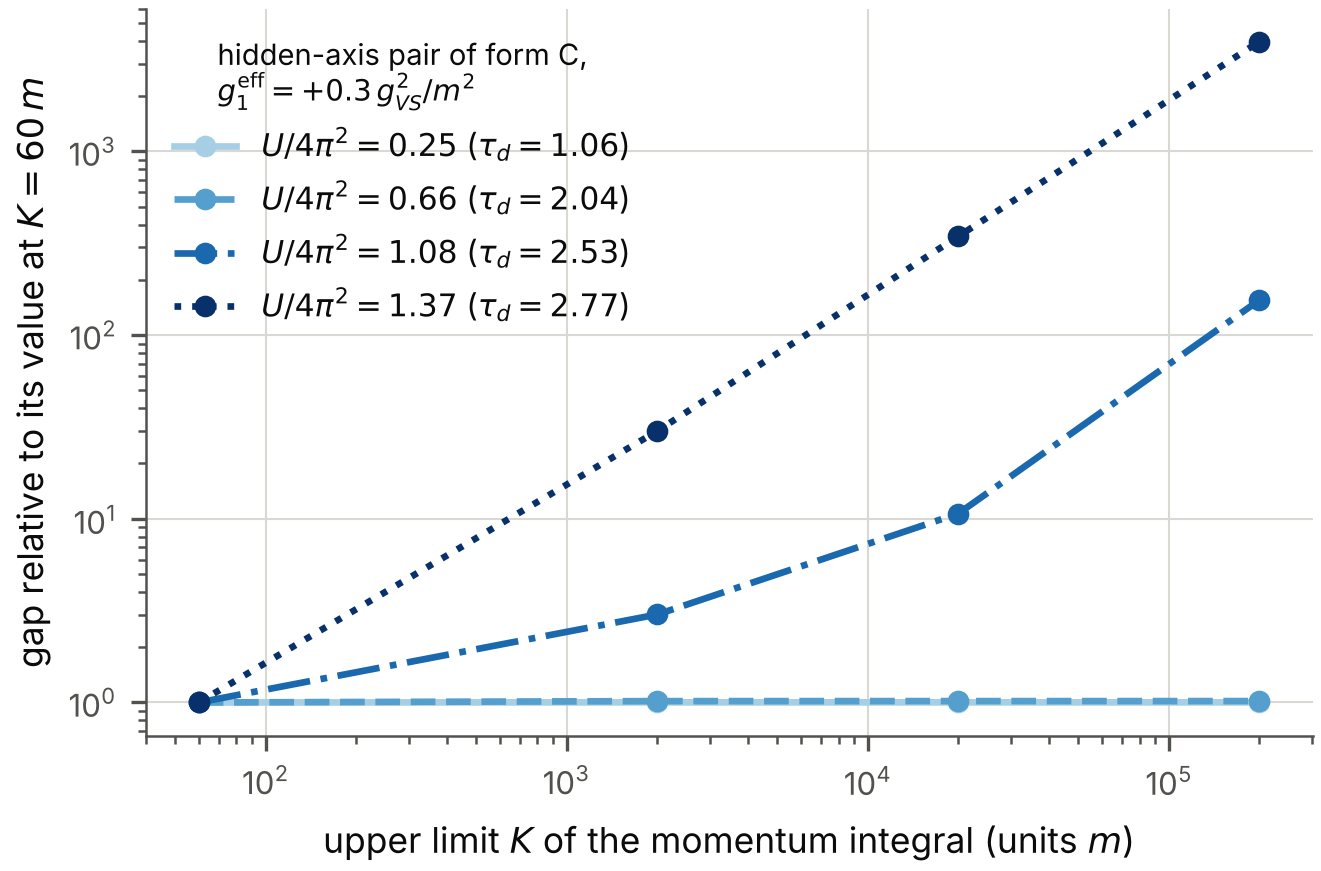
\includegraphics[width=0.62\textwidth,height=\textheight]{../figures/fig_forms_uv.png}
\caption{The gap as a function of the upper limit \(K\) of the momentum
integral, relative to its value at \(K=60\,m\), for the hidden-axis pair
of form C with the vector contact coupling \(+0.3\,g_{VS}^2/m^2\)
(\(m_s=m\), \(k_F=0.5\,m\)) at four clock readings. Below the criterion
(\(U/4\pi^2<1\), the two lower curves, which coincide on this scale) the
gap does not depend on the limit; above it the gap grows with the limit
without bound.}
\end{figure}

By classes of the ultraviolet strength, for the cases below the
criterion:

\begin{longtable}[]{@{}
  >{\raggedright\arraybackslash}p{(\columnwidth - 6\tabcolsep) * \real{0.2500}}
  >{\raggedleft\arraybackslash}p{(\columnwidth - 6\tabcolsep) * \real{0.2500}}
  >{\raggedleft\arraybackslash}p{(\columnwidth - 6\tabcolsep) * \real{0.2500}}
  >{\raggedleft\arraybackslash}p{(\columnwidth - 6\tabcolsep) * \real{0.2500}}@{}}
\toprule\noalign{}
\begin{minipage}[b]{\linewidth}\raggedright
ultraviolet strength
\end{minipage} & \begin{minipage}[b]{\linewidth}\raggedleft
cases
\end{minipage} & \begin{minipage}[b]{\linewidth}\raggedleft
change of the gap from \(K=2\times10^4\) to \(2\times10^5\) (relative)
\end{minipage} & \begin{minipage}[b]{\linewidth}\raggedleft
error of the limit \(K=60\) (per cent)
\end{minipage} \\
\midrule\noalign{}
\endhead
\bottomrule\noalign{}
\endlastfoot
\(U/4\pi^2<0.5\) & 118 & \(2.5\times10^{-6}\) & 0.75 \\
\(0.5\) to \(0.7\) & 28 & \(6.4\times10^{-5}\) & 2.37 \\
\(0.7\) to \(0.9\) & 8 & \(3.3\times10^{-3}\) & 12.59 \\
\end{longtable}

Above the criterion (8 cases) the gap grows by a factor between 11.49
and 14.56 from \(K=2\times10^4\) to \(2\times10^5\); its value then
depends on the limit and on the grid of momenta, and is not a property
of the model. \textbf{All gaps of this folder are computed with
\(K=2\times10^4\), and none is given above the criterion.} The earlier
calculations of the project used \(K=60\); their gaps of the exchange of
the Vorton-Scalar alone are too small by up to 1.08 per cent at the
strongest coupling (\(g_{VS}=4\)), and their gaps with contact couplings
by the percentages of the last column.

\begin{center}\rule{0.5\linewidth}{0.5pt}\end{center}

\hypertarget{symmetries}{%
\section{8. Symmetries}\label{symmetries}}

\hypertarget{the-frame-group}{%
\subsection{8.1 The frame group}\label{the-frame-group}}

The 28 matrices \(\tfrac12\gamma^A\gamma^B\) (\(A<B\)) generate the
rotations and boosts of the 4+4 frame. The invariants \(I_r^{\rm C}\) of
form C are invariant under all 28 (check \texttt{44c-S4}). The positive
kinetic and mass terms (2.5) are invariant only under the 13 generators
that commute with \(W\): the ten rotations and boosts of \(x0,\dots,x4\)
and the three rotations of \(x5,x6,x7\). The other fifteen generators
mix a space-like coordinate or the ordinary time with an extra time;
they do not preserve the quantized sector (a field that does not depend
on \(x5,x6,x7\) is turned into one that does).

The invariants \(I_r^{\rm Q}\) of form Q are invariant under the 28
matrices \(\tfrac12\gamma_{44q}^A\gamma_{44q}^B\), which generate the
group of a spacetime with one time. Thirteen of them are the thirteen
transformations just named; the other fifteen mix the two halves of the
field and are not transformations of the coordinates of the 4+4
spacetime (check \texttt{44q-S4}).

Both models, as wholes, have the same thirteen symmetries of the
coordinates. The difference is in the quartic term alone: that of form C
is invariant under the full group of the 4+4 frame, as the hypothesis of
the project requires of ``the invariants of the spacetime''; that of
form Q is invariant under a different group of the same size, which is
not a symmetry group of the 4+4 spacetime.

\hypertarget{the-internal-symmetry-of-fields-in-ordinary-space}{%
\subsection{8.2 The internal symmetry of fields in ordinary
space}\label{the-internal-symmetry-of-fields-in-ordinary-space}}

A field that depends on \(x1,x2,x3,x4\) only has a kinetic term that
contains \(\alpha^1,\alpha^2,\alpha^3\) and \(\beta\). Eight Hermitian
matrices commute with these four: the six generators
\(\propto\gamma^a\gamma^b\) (\(a<b\) in \(\{0,5,6,7\}\)) of the
rotations of the four extra axes, which form \(SO(4)\); the unit matrix
(the fermion number); and
\(P_E\propto\gamma^0\gamma^5\gamma^6\gamma^7\), which generates a second
phase symmetry called \(U(1)_E\). The model with the Vorton-Scalar and
without contact self-interaction is invariant under all eight. The three
rotations of \(x5,x6,x7\) among themselves commute with \(W\); the three
generators \(\gamma^0\gamma^t\) and \(P_E\) anticommute with \(W\) and
connect the two halves.

Under which couplings is the self-interaction invariant under the
unitary transformation \(\psi\to e^{i\theta T}\psi\) generated by each
of them? In exact arithmetic (checks \texttt{71s-S12}, \texttt{44q-S12},
\texttt{44c-S12}; confirmed at a finite angle by the independent script,
check \texttt{Icks-F2}):

\begin{longtable}[]{@{}
  >{\raggedright\arraybackslash}p{(\columnwidth - 8\tabcolsep) * \real{0.2000}}
  >{\raggedleft\arraybackslash}p{(\columnwidth - 8\tabcolsep) * \real{0.2000}}
  >{\raggedright\arraybackslash}p{(\columnwidth - 8\tabcolsep) * \real{0.2000}}
  >{\raggedright\arraybackslash}p{(\columnwidth - 8\tabcolsep) * \real{0.2000}}
  >{\raggedright\arraybackslash}p{(\columnwidth - 8\tabcolsep) * \real{0.2000}}@{}}
\toprule\noalign{}
\begin{minipage}[b]{\linewidth}\raggedright
generators
\end{minipage} & \begin{minipage}[b]{\linewidth}\raggedleft
number
\end{minipage} & \begin{minipage}[b]{\linewidth}\raggedright
\(7+1\)
\end{minipage} & \begin{minipage}[b]{\linewidth}\raggedright
\(4+4\), form Q
\end{minipage} & \begin{minipage}[b]{\linewidth}\raggedright
\(4+4\), form C
\end{minipage} \\
\midrule\noalign{}
\endhead
\bottomrule\noalign{}
\endlastfoot
phase of the field (fermion number) & 1 & all couplings & all couplings
& all couplings \\
rotations of \(x5,x6,x7\) among themselves & 3 & all couplings & all
couplings & all couplings \\
rotations that mix \(x0\) with \(x5\), \(x6\) or \(x7\) & 3 & all
couplings & all couplings & no coupling
(\(g_0^{\rm eff}=g_1^{\rm eff}=g_7^{\rm eff}=g_8^{\rm eff}=0\)) \\
\(P_E\), the generator of \(U(1)_E\) & 1 &
\(g_1^{\rm eff}=g_7^{\rm eff}=0\) & \(g_1^{\rm eff}=g_7^{\rm eff}=0\) &
no coupling
(\(g_0^{\rm eff}=g_1^{\rm eff}=g_7^{\rm eff}=g_8^{\rm eff}=0\)) \\
\end{longtable}

\begin{quote}
\textbf{In form C every self-interaction that does not vanish breaks the
three transformations that mix the hidden axis with \(x5,x6,x7\), and
breaks \(U(1)_E\).} The internal symmetry of fields in ordinary space is
reduced from \(SO(4)\times U(1)\times U(1)_E\) to
\(SO(3)_T\times U(1)\): the rotations of the three extra time-like
coordinates among themselves, and the fermion number.
\end{quote}

The four conditions of the table for form C,
\(5g_0^{\rm eff}-16g_7^{\rm eff}+g_8^{\rm eff}=0\),
\(5g_1^{\rm eff}-4g_7^{\rm eff}-g_8^{\rm eff}=0\),
\(4g_7^{\rm eff}+g_8^{\rm eff}=0\) and
\(g_7^{\rm eff}-g_8^{\rm eff}=0\), have only the solution in which all
four effective couplings vanish.

\emph{Why.} In the frame group of the 4+4 spacetime \(\gamma^0\gamma^t\)
generates a \textbf{boost} (it mixes a space-like with a time-like
coordinate), which is not a unitary transformation of the field. The
\emph{unitary} transformation \(e^{i\theta\gamma^0\gamma^t}\) is a
different transformation: it is a symmetry of the kinetic term of fields
in ordinary space by accident, and it is not an element of the frame
group. The quartic term of form C is invariant under the boost and has
no reason to be invariant under the unitary transformation. In form Q,
as on the 7+1 spacetime, where all four extra axes are space-like, the
same matrices generate rotations, which are unitary, and the quartic
term is invariant under them.

\emph{What this means for the pairs.} It is the symmetry statement
behind Section 7: in form Q the pair along \(x0\) can be rotated into
the pairs along \(x5,x6,x7\), so that they are degenerate; in form C it
cannot, and they are not.

\hypertarget{the-chiral-condition}{%
\subsection{8.3 The chiral condition}\label{the-chiral-condition}}

Under \(\psi\to e^{i\epsilon\chi}\psi\) the self-interaction is
invariant if and only if

\[g_0^{\rm eff}+g_8^{\rm eff}=0\quad\text{(form Q, and 7+1)},\qquad
g_1^{\rm eff}-g_7^{\rm eff}=0\quad\text{(form C)}\tag{8.1}\]

(checks \texttt{44q-S10}, \texttt{44c-S10}). The roles of the even and
the odd ranks are exchanged, because the bilinears of the two forms
differ by the matrix \(W\), which anticommutes with \(\chi\). A scalar
coupling alone (\(g_0\neq0\)) is chirally invariant in form C and not in
form Q; a vector coupling alone is chirally invariant in form Q and not
in form C. The mass term breaks the chiral symmetry in both forms.

\hypertarget{consequence-for-the-hypothesis-that-the-pair-condensate-is-the-higgs-field}{%
\subsection{8.4 Consequence for the hypothesis that the pair condensate
is the Higgs
field}\label{consequence-for-the-hypothesis-that-the-pair-condensate-is-the-higgs-field}}

One of the author's hypotheses identifies the pair condensate along the
hidden axis with the Higgs field: the six generators of the \(SO(4)\) of
Section 8.2 would play the role of the electroweak group, and the
condensate along \(x0\) would break it to the \(SO(3)\) of the rotations
of \(x5,x6,x7\), as the Higgs vacuum breaks the electroweak group.

In form Q this pattern is present in the sector of fields in ordinary
space for any couplings of the self-interaction, as a hidden symmetry
(it is not a symmetry of the 4+4 spacetime). In form C it is not: the
self-interaction itself breaks \(SO(4)\) to \(SO(3)_T\)
\emph{explicitly}. The three generators that the condensate would have
to break spontaneously are not symmetries of the model; no massless
modes of the order parameter correspond to them; and by Section 7 the
condensate along \(x0\) is not degenerate with those along \(x5,x6,x7\).
The pattern survives in form C only in the model without contact
self-interaction (the exchange of the Vorton-Scalar keeps the whole
internal symmetry).

\begin{center}\rule{0.5\linewidth}{0.5pt}\end{center}

\hypertarget{the-vorton-scalar}{%
\section{9. The Vorton-Scalar}\label{the-vorton-scalar}}

The Yukawa coupling of the complex scalar field \(\phi\) of the project
to the fermions contains \(\bar\psi\psi\) and \(\bar\psi\,i\chi\,\psi\)
with \(\bar\psi=\psi^\dagger\beta\). Under the chiral rotation
\(\psi\to e^{i\epsilon\chi}\psi\) these two bilinears rotate into each
other, and the coupling is invariant when the phase of \(\phi\) rotates
with them; the phase mode of the scalar is the Goldstone mode of this
symmetry. The covariant bilinears cannot take this role: \(C^-\)
commutes with \(\chi\), so that \(\tilde\psi\psi\) and
\(\tilde\psi\,\chi\,\psi\) are each invariant under the chiral rotation
and do not couple to the phase of a complex field. The Yukawa coupling
is therefore written with \(\bar\psi\) in both forms, and an expectation
value of the scalar shifts the masses of both halves by the same amount.

With a bare Dirac mass \(m_D\), a Yukawa mass \(m_Y\) (\(m=m_D+m_Y\) in
vacuum, \(f_D=m_D/m\)) and the self-interaction, the energy density of
uniform matter is

\[\varepsilon=\frac{(1-f_D)^2\,(x^2-1)^2}{8\,C}+\varepsilon_{\rm halves}\big[m\to f_D+(1-f_D)\,x\big],\tag{9.1}\]

where \(x=\phi/v_{VS}\) is the expectation value of the scalar in units
of its vacuum value, \(C=g_{VS}^2m^2/m_s^2\) its coupling, and
\(\varepsilon_{\rm halves}\) the energy density (5.9) with the mass
\(m\) replaced as shown (units \(m=1\), \(D=3\)). The smallest \(C\) at
which matter is self-bound, with the contact couplings
\(g_0=-\kappa_0\,C\) and \(g_1=+\kappa_1\,C\), is (\(\Delta\tau_d\): the
shift of the clock reading against the model without bare mass and
self-interaction, where \(C=3\pi^2/8\); \(x\): the value of the scalar
field in the bound state just above the threshold):

\begin{longtable}[]{@{}
  >{\raggedleft\arraybackslash}p{(\columnwidth - 12\tabcolsep) * \real{0.0833}}
  >{\raggedleft\arraybackslash}p{(\columnwidth - 12\tabcolsep) * \real{0.0694}}
  >{\raggedleft\arraybackslash}p{(\columnwidth - 12\tabcolsep) * \real{0.0694}}
  >{\raggedleft\arraybackslash}p{(\columnwidth - 12\tabcolsep) * \real{0.2778}}
  >{\raggedleft\arraybackslash}p{(\columnwidth - 12\tabcolsep) * \real{0.1111}}
  >{\raggedleft\arraybackslash}p{(\columnwidth - 12\tabcolsep) * \real{0.2778}}
  >{\raggedleft\arraybackslash}p{(\columnwidth - 12\tabcolsep) * \real{0.1111}}@{}}
\toprule\noalign{}
\begin{minipage}[b]{\linewidth}\raggedleft
\(f_D\)
\end{minipage} & \begin{minipage}[b]{\linewidth}\raggedleft
\(\kappa_0\)
\end{minipage} & \begin{minipage}[b]{\linewidth}\raggedleft
\(\kappa_1\)
\end{minipage} & \begin{minipage}[b]{\linewidth}\raggedleft
form C: \(C\) (\(\Delta\tau_d\))
\end{minipage} & \begin{minipage}[b]{\linewidth}\raggedleft
\(x\)
\end{minipage} & \begin{minipage}[b]{\linewidth}\raggedleft
form Q: \(C\) (\(\Delta\tau_d\))
\end{minipage} & \begin{minipage}[b]{\linewidth}\raggedleft
\(x\)
\end{minipage} \\
\midrule\noalign{}
\endhead
\bottomrule\noalign{}
\endlastfoot
0 & 0 & 0 & 3.7011 (\(0\)) & 0.000 & 3.7011 (\(0\)) & 0.000 \\
0 & 1 & 0 & 3.9399 (\(+0.063\)) & 0.000 & 3.7156 (\(+0.004\)) & 0.614 \\
0 & 1 & 0.1 & 3.9399 (\(+0.063\)) & 0.000 & 4.1527 (\(+0.115\)) &
0.652 \\
0.25 & 0 & 0 & 2.5112 (\(-0.388\)) & 0.000 & 2.5112 (\(-0.388\)) &
0.000 \\
0.25 & 1 & 0 & 2.6336 (\(-0.340\)) & 0.000 & 2.4758 (\(-0.402\)) &
0.000 \\
0.25 & 1 & 0.1 & 2.6307 (\(-0.341\)) & 0.000 & 2.6992 (\(-0.316\)) &
0.000 \\
0.5 & 0 & 0 & 2.0643 (\(-0.584\)) & 0.000 & 2.0643 (\(-0.584\)) &
0.000 \\
0.5 & 1 & 0 & 2.1617 (\(-0.538\)) & 0.000 & 1.8252 (\(-0.707\)) &
0.000 \\
0.5 & 1 & 0.1 & 2.1559 (\(-0.540\)) & 0.000 & 1.9335 (\(-0.649\)) &
0.000 \\
\end{longtable}

In all 18 cases the bound state at the threshold has equal halves, in
both forms: the attraction that binds it is that of the scalar field,
which acts on both halves alike, and the contact couplings of these
strengths are too weak to polarize it. The threshold is that of matter
of one kind with the couplings \(T_S,T_V\) of the form, confirmed with
the functional of two halves minimized over the density, the field and
the polarization (bound 0.1 per cent above, with \(\varepsilon/n-m\) at
least \(1.6\times10^{-4}\) \(m\) above zero 0.1 per cent below; check
\texttt{fm-F8}). The forms differ because the couplings of the total
densities differ (table of Section 5.2). In form Q the scalar contact
coupling adds its attraction \(G_S^{\rm HF}\) to that of the scalar
field, and a vector coupling adds the repulsion \(G_V^{\rm HF}\). In
form C the couplings of the total densities are \(G_S^{\rm c}\) and
\(G_V^{\rm c}\), both small, so that the contact couplings change the
threshold less. Which form binds earlier depends on the case. Without
bare mass the bound state of form C at the threshold has \(x=0\): the
fermions are massless in it, the scalar densities vanish, and the
threshold does not depend on the vector coupling of set B.

\begin{center}\rule{0.5\linewidth}{0.5pt}\end{center}

\hypertarget{gravity}{%
\section{10. Gravity}\label{gravity}}

\textbf{The equations.} Let the three rates be equal,
\(\mathrm{g55}=\mathrm{g66}=\mathrm{g77}\), and let the four space-like
coordinates have a scale factor of their own:

\[ds^2=-(dx4)^2+\mathsf a(x4)^2\sum_{j=0}^{3}(dxj)^2-\mathsf b(x4)^2\sum_{t=5}^{7}(dxt)^2,\qquad
H_{\mathsf a}=\frac{\mathsf a'}{\mathsf a},\quad H_{\mathsf b}=\frac{\mathsf b'}{\mathsf b}\tag{10.1}\]

(a prime is a derivative with respect to \(x4\)). The deflating
spacetime of the hypothesis is \(\mathsf a=1\),
\(H_{\mathsf b}=-\mathrm{g55}\); it is called the \emph{undisturbed
deflation}. For such a metric the curvature is determined by one number
for each pair of directions of the frame,

\[K_{4i}=H_i'+H_i^2,\qquad K_{ij}=H_i\,H_j\quad(i\neq j),\tag{10.2}\]

where \(i,j\) run over the seven directions other than the time and
\(H_i\) is the rate of the direction \(i\). The field equations of
second order for the metric in eight dimensions are the
Einstein--Lovelock equations,

\[\sum_{k=1}^{3}\alpha_k\,E^{(k)\mu}{}_{\nu}-\bar\Lambda\,\delta^\mu_\nu=\kappa_8\,T^\mu{}_\nu,\qquad\alpha_1=1,\tag{10.3}\]

\[E^{(k)m}{}_{m}=(-1)^{k+1}\,k!\,2^{k-1}\sum_{\text{sets of }2k\text{ directions}\neq m}\ \ \sum_{\text{divisions into pairs}}\ \prod_{\text{pairs}}K_{\rm pair}\tag{10.4}\]

(no summation over \(m\); \(E^{(1)}\) is minus the Einstein tensor),
with the couplings \(\alpha_2,\alpha_3\) of the two higher terms, the
cosmological term \(\bar\Lambda\) and the gravitational coupling
\(\kappa_8\). The energy-momentum tensor of uniform matter has
\(T^4{}_4=\varepsilon\) and \(T^m{}_m=-p_m\), with the pressure \(p\) of
Eq. (5.10) along \(x0,\dots,x3\) and the interaction pressure \(\Pi\)
along \(x5,x6,x7\). Without matter the undisturbed deflation solves Eq.
(10.3) if and only if

\[\bar\Lambda=3\,\mathrm{g55}^2,\qquad\alpha_2=\frac1{4\,\mathrm{g55}^2}\tag{10.5}\]

(\(\alpha_3\) arbitrary): the \emph{tuned} Einstein--Lovelock gravity.
\emph{Einstein gravity} is \(\alpha_2=\alpha_3=0\), \(\bar\Lambda=0\),
with the matter as the only source. The \textbf{loading} of an evolution
is the number \(\kappa_8\,\varepsilon(0)/(3\,\mathrm{g55}^2)\), the
energy density of the matter at the start in the unit that the deflation
sets.

\textbf{The matter of the two forms as the source} (fields of the
quantized sector, \(D=4\), set B, three times the binding threshold of
each form):

\begin{longtable}[]{@{}
  >{\raggedright\arraybackslash}p{(\columnwidth - 10\tabcolsep) * \real{0.1667}}
  >{\raggedleft\arraybackslash}p{(\columnwidth - 10\tabcolsep) * \real{0.1667}}
  >{\raggedright\arraybackslash}p{(\columnwidth - 10\tabcolsep) * \real{0.1667}}
  >{\raggedleft\arraybackslash}p{(\columnwidth - 10\tabcolsep) * \real{0.1667}}
  >{\raggedleft\arraybackslash}p{(\columnwidth - 10\tabcolsep) * \real{0.1667}}
  >{\raggedleft\arraybackslash}p{(\columnwidth - 10\tabcolsep) * \real{0.1667}}@{}}
\toprule\noalign{}
\begin{minipage}[b]{\linewidth}\raggedright
form
\end{minipage} & \begin{minipage}[b]{\linewidth}\raggedleft
threshold \(g\,m^3\)
\end{minipage} & \begin{minipage}[b]{\linewidth}\raggedright
state at 3 times the threshold
\end{minipage} & \begin{minipage}[b]{\linewidth}\raggedleft
\(k_F/m\) of the filled states
\end{minipage} & \begin{minipage}[b]{\linewidth}\raggedleft
\(M/m\)
\end{minipage} & \begin{minipage}[b]{\linewidth}\raggedleft
\(\varepsilon/n-m\) (units \(m\))
\end{minipage} \\
\midrule\noalign{}
\endhead
\bottomrule\noalign{}
\endlastfoot
C & 332.2917 & one half filled & 0.52859 & 0.37920 & \(-0.09072\) \\
Q & 121.0858 & equal halves & 0.58171 & 0.35844 & \(-0.10601\) \\
\end{longtable}

\begin{figure}
\centering
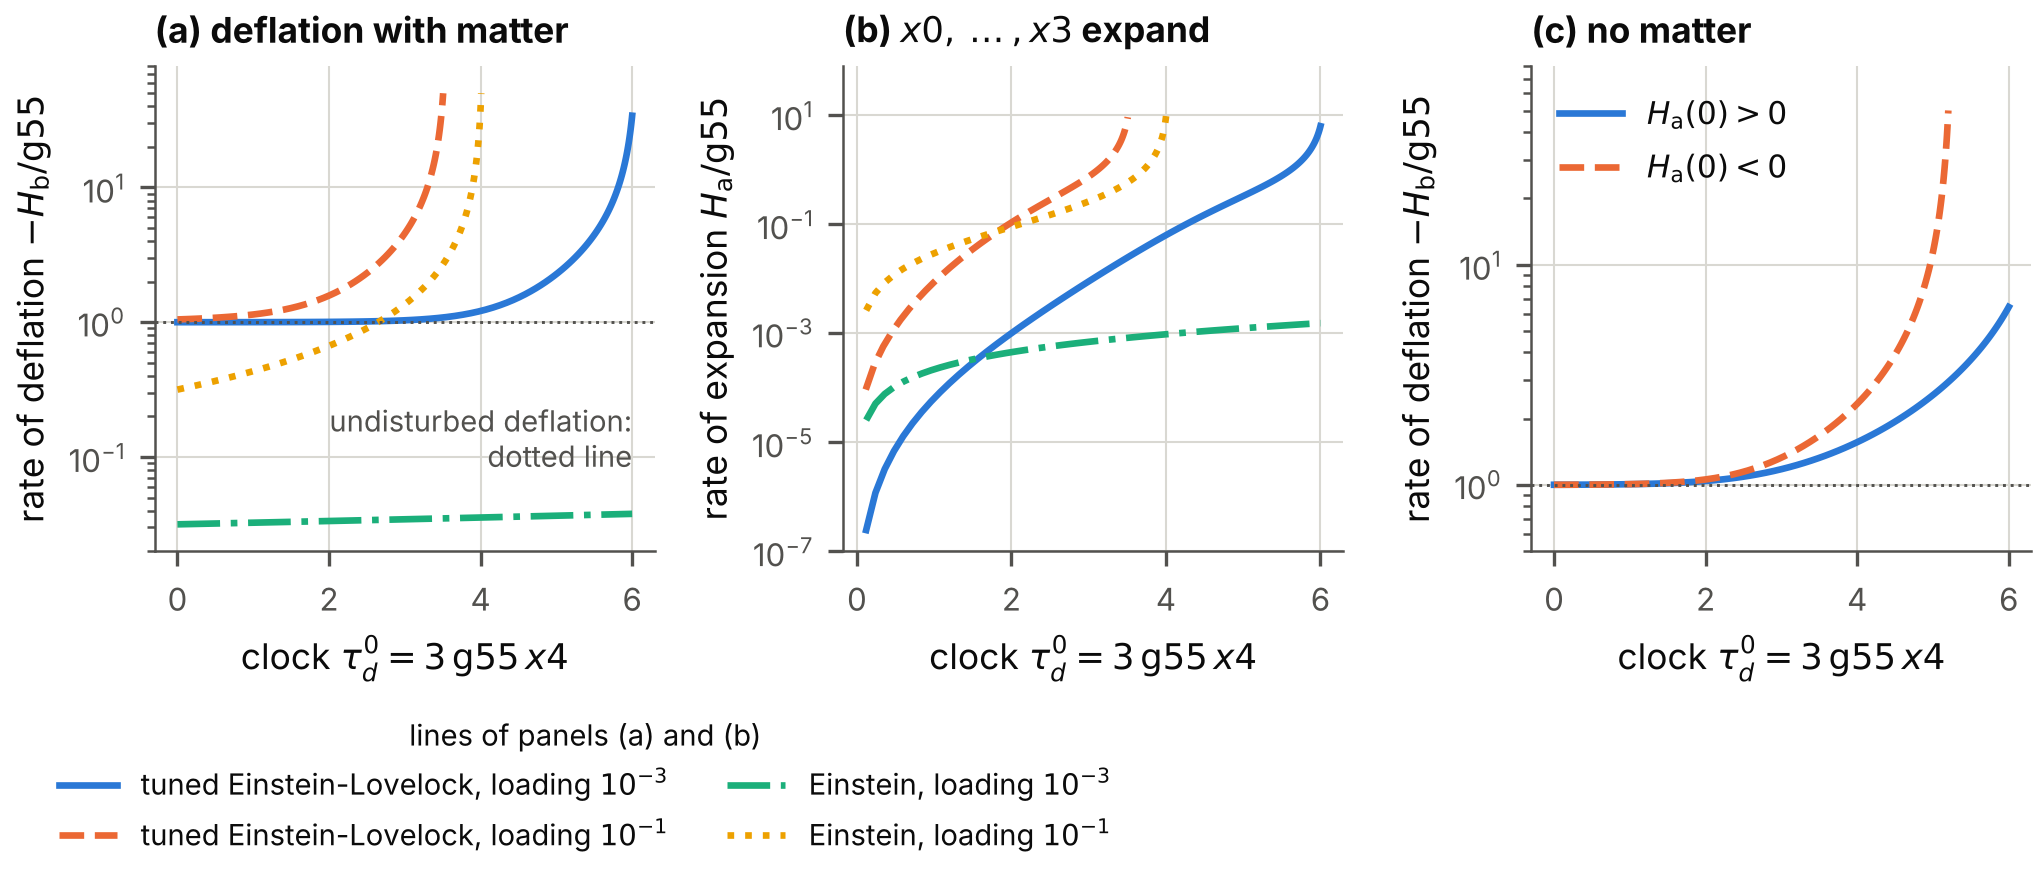
\includegraphics[width=0.96\textwidth,height=\textheight]{../figures/fig_gravity_deflating_formC.png}
\caption{The deflating 4+4 spacetime with the matter of form C (one half
filled) as a source of gravity. (a) The rate of deflation
\(-H_{\mathsf b}\) of \(x5,x6,x7\) in units of its undisturbed value
\(\mathrm{g55}\), along the clock \(3\,\mathrm{g55}\,x4\) of the
undisturbed deflation; (b) the rate \(H_{\mathsf a}\) at which the
coordinates \(x0,\dots,x3\) expand; four evolutions: the tuned
Einstein--Lovelock gravity and Einstein gravity, each with the loadings
\(10^{-3}\) and \(10^{-1}\). (c) The same spacetime without matter in
the tuned gravity, slightly disturbed. The deflation does not return to
its undisturbed rate in any of the evolutions.}
\end{figure}

In an evolution without collisions every particle keeps its state, so
that a half that is empty stays empty. The matter of form C is then
matter of one kind of particle with four internal states and the
couplings \(a_S\), \(a_V\) throughout the evolution; the matter of form
Q is matter of one kind with eight states and the couplings
\(G_S^{\rm HF}\), \(G_V^{\rm HF}\). Both were computed again with the
routines for matter of one kind (other integrals), with agreement to
\(1.3\times10^{-15}\) (check \texttt{gr-G6}). In the evolutions (Figure
7 for form C) the two kinds of matter behave alike in kind: the
conclusions on the stability of the deflation do not depend on the form.
With the tuned Einstein--Lovelock gravity and the loading \(10^{-3}\)
the rate of the deflating coordinates at the end of the evolution is
34.1 times its initial value for the matter of form C and 15.6 times for
the matter of form Q.

\begin{center}\rule{0.5\linewidth}{0.5pt}\end{center}

\hypertarget{discussion-of-the-two-options}{%
\section{11. Discussion of the two
options}\label{discussion-of-the-two-options}}

\hypertarget{what-each-option-is}{%
\subsection{11.1 What each option is}\label{what-each-option-is}}

Both options keep what the quantum theory needs: the positive kinetic
term, a real (Hermitian) interaction, and the conservation of the number
of particles. Both use the same nine couplings and the same four
effective couplings. They assign to these couplings different meanings.
Form C takes the hypothesis literally: the quartic term is built from
the invariants of the 4+4 spacetime. Form Q takes the \emph{particle
content} literally: the eight internal states of a particle are treated
alike, as on the 7+1 spacetime.

\hypertarget{arguments-for-form-c}{%
\subsection{11.2 Arguments for form C}\label{arguments-for-form-c}}

\begin{enumerate}
\def\labelenumi{\arabic{enumi}.}
\tightlist
\item
  \textbf{It is the quartic term of the hypothesis.} The invariants
  \(I_r^{\rm C}\) are the ones that are invariant under all rotations
  and boosts of the 4+4 frame. They can be written on the full deflating
  spacetime, for fields that depend on all eight coordinates, with the
  spin connection; the quantized sector is a restriction of that
  covariant theory. Form Q is defined in the quantized sector only: its
  invariance group is not a symmetry group of the 4+4 spacetime, and it
  has no covariant extension to fields that depend on the extra times.
\item
  \textbf{Its dynamics respects the distinction that the metric makes.}
  On the 4+4 spacetime \(x0\) is space-like and \(x5,x6,x7\) are
  time-like. Form C treats them differently (Sections 7 and 8); form Q
  has an accidental symmetry that rotates them into one another.
\item
  \textbf{Each structure appears with its own adjoint.} The mass that
  the interaction of form C generates in vacuum is the covariant mass
  term (Section 6.2).
\end{enumerate}

\hypertarget{arguments-against-form-c-or-for-form-q}{%
\subsection{11.3 Arguments against form C, or for form
Q}\label{arguments-against-form-c-or-for-form-q}}

\begin{enumerate}
\def\labelenumi{\arabic{enumi}.}
\tightlist
\item
  \textbf{The two adjoints are mixed.} Form C combines the quartic term
  of the covariant Lagrangian with the kinetic and mass terms of the
  positive Lagrangian. The Lagrangian as a whole is invariant only under
  the thirteen generators that both parts share, the same thirteen as
  for form Q. The covariance of the quartic term is not a symmetry of
  the model.
\item
  \textbf{The bare mass term and the dynamical mass have different
  structures} in form C. With a bare mass the vacuum has a sharp
  transition at which the symmetry between the halves breaks
  spontaneously (Section 6.3). In form Q the two have the same
  structure.
\item
  \textbf{The results of the 7+1 spacetime do not carry over.} In form Q
  every result for fields that do not depend on \(x5,x6,x7\) is the same
  on the two spacetimes; in form C the 4+4 model is a different model,
  with polarized matter, later binding, and pairs that are not
  degenerate.
\item
  \textbf{The pattern of the Higgs hypothesis is lost} as soon as there
  is a contact self-interaction (Section 8.4), and with an attractive
  scalar coupling the condensate does not form along the hidden axis
  (Section 7.5).
\item
  \textbf{A scalar coupling of the sign that binds matter on 7+1 binds
  less.} Matter needs two to three times the strength (Section 5.5),
  which moves it further outside the range in which the no-sea
  approximation is controlled (Section 6.4).
\end{enumerate}

\hypertarget{what-does-not-distinguish-them}{%
\subsection{11.4 What does not distinguish
them}\label{what-does-not-distinguish-them}}

\begin{itemize}
\tightlist
\item
  The reduction to four effective couplings, the Fierz matrix and all
  algebra of Section 4.3.
\item
  The interaction between particles of the same half, hence everything
  about matter that occupies one half only.
\item
  The pairs along \(x5,x6,x7\).
\item
  The exchange of the Vorton-Scalar, hence every result of the project
  that does not involve the contact self-interaction.
\item
  The equivalence of the Kohn--Sham and the CJT method.
\item
  The conclusions on gravity (Section 10).
\item
  The critical strength at which the vacuum of a massless field becomes
  unstable, and the magnitude of the mass that it acquires.
\end{itemize}

\hypertarget{what-could-decide}{%
\subsection{11.5 What could decide}\label{what-could-decide}}

Three kinds of consideration could decide between the options; none of
them is settled by the calculations of this folder.

\begin{enumerate}
\def\labelenumi{\arabic{enumi}.}
\tightlist
\item
  \emph{A principle.} If the model is required to be the restriction of
  a covariant theory on the full 4+4 spacetime, form C follows. If it is
  required to be the theory of eight equivalent internal states, form Q
  follows.
\item
  \emph{A consistent quantization of the covariant Lagrangian itself.}
  If a quantization of Eq. (2.1) with its indefinite sign existed (with
  an indefinite metric on the space of states and a rule for the
  physical states), it would dictate the form of the interaction, and it
  would give neither form C nor form Q in general (Section 3.4). No such
  quantization is constructed in this project.
\item
  \emph{An observable consequence.} The two forms differ in the internal
  states of self-bound matter (four or eight), in the direction of the
  condensate, and in the symmetry of the order parameter. A hypothesis
  of the project that ties one of these to an observation would select a
  form.
\end{enumerate}

\begin{center}\rule{0.5\linewidth}{0.5pt}\end{center}

\hypertarget{what-has-been-established-and-what-has-not}{%
\section{12. What has been established, and what has
not}\label{what-has-been-established-and-what-has-not}}

\textbf{Established (exact algebra, verified by the program in integer
arithmetic and independently by a second program):}

\begin{itemize}
\tightlist
\item
  the two forms are related by the insertion of \(W\) in every bilinear
  (4.1), (4.2);
\item
  the five linear relations among the nine invariants and the four
  effective couplings are the same in both forms;
\item
  in matter without coherence between the halves the Hartree--Fock
  energy is the sum of four squares (5.3), with the same four
  combinations of couplings in both forms and the roles of the totals
  and the differences exchanged;
\item
  the pair couplings of the 28 pairs at rest, and the sign rule (7.4) of
  the contact amplitudes at all momenta;
\item
  the conditions of invariance under the internal symmetry and under the
  chiral rotation, in both forms; in particular that every
  self-interaction of form C breaks \(SO(4)\times U(1)_E\) to
  \(SO(3)_T\);
\item
  the ultraviolet criterion \(U<4\pi^2\) of the gap equation and the
  formula (7.10).
\end{itemize}

\textbf{Established numerically (each by two methods or two programs):}

\begin{itemize}
\tightlist
\item
  matter of form C is polarized, and self-bound matter has one filled
  half; matter of form Q is not polarized; the binding thresholds and
  the saturated states along the clock for the sets A and B;
\item
  the vacuum of a massless field acquires masses of opposite sign in the
  two halves in form C and of equal sign in form Q, at the same critical
  strength; with a bare mass form C has a sharp transition;
\item
  the gaps of the two kinds of pairs with contact couplings, and their
  dependence on the upper limit of the momentum integral.
\end{itemize}

\textbf{Not established:}

\begin{itemize}
\tightlist
\item
  \emph{States with coherence between the halves.} The density matrix
  (5.1) is diagonal in \(W\). Because the interaction connects the
  halves, states in which
  \(\langle\psi_+^\dagger\,\cdot\,\psi_-\rangle\neq0\) are possible in
  principle, in both forms; whether one of them has a lower energy than
  the states found here has not been examined. The statements of Section
  5 are statements about the states of the form (5.1).
\item
  \emph{Other couplings.} The numbers are for the sets A and B (scalar
  attraction, with and without a small vector repulsion). The exact
  formulas hold for all couplings; the numerical statements have not
  been extended to couplings with \(g_7\) or \(g_8\).
\item
  \emph{Beyond the mean field.} All results on matter and on the vacuum
  are in the Hartree--Fock approximation (equivalently, the CJT
  effective action in the double-bubble truncation), and those on matter
  in the no-sea approximation, which at the binding thresholds is
  outside its controlled range (Section 6.4).
\item
  \emph{Solutions with a negative mass.} Where the gap equations of
  matter have no solution with non-negative masses (Section 5.4), the
  continuation with a mass that has changed its sign has not been
  followed.
\item
  \emph{Which form is right.} Section 11.5.
\end{itemize}

\begin{center}\rule{0.5\linewidth}{0.5pt}\end{center}

\hypertarget{where-the-two-forms-are-recorded-and-how-to-repeat-every-number}{%
\section{13. Where the two forms are recorded, and how to repeat every
number}\label{where-the-two-forms-are-recorded-and-how-to-repeat-every-number}}

\hypertarget{in-the-program}{%
\subsection{13.1 In the program}\label{in-the-program}}

The program of this folder is the Rust crate
\texttt{code/deflation-cjt-ks-c-rs} (binary
\texttt{deflation\_cjt\_ks\_c}). Nothing of form Q was removed from it;
form C stands beside it and is labeled as the definition.

\begin{longtable}[]{@{}
  >{\raggedright\arraybackslash}p{(\columnwidth - 6\tabcolsep) * \real{0.2917}}
  >{\raggedright\arraybackslash}p{(\columnwidth - 6\tabcolsep) * \real{0.2083}}
  >{\raggedright\arraybackslash}p{(\columnwidth - 6\tabcolsep) * \real{0.2083}}
  >{\raggedright\arraybackslash}p{(\columnwidth - 6\tabcolsep) * \real{0.2917}}@{}}
\toprule\noalign{}
\begin{minipage}[b]{\linewidth}\raggedright
object
\end{minipage} & \begin{minipage}[b]{\linewidth}\raggedright
form C
\end{minipage} & \begin{minipage}[b]{\linewidth}\raggedright
form Q
\end{minipage} & \begin{minipage}[b]{\linewidth}\raggedright
source file
\end{minipage} \\
\midrule\noalign{}
\endhead
\bottomrule\noalign{}
\endlastfoot
the 256 matrices, exact algebra & model \texttt{S44C}, tag \texttt{44c}
& model \texttt{S44Q}, tag \texttt{44q} & \texttt{src/selfint.rs} \\
mean-field couplings of two halves & \texttt{Form::C} & \texttt{Form::Q}
& \texttt{src/halves.rs} \\
matter of two halves, vacuum, functional with the scalar &
\texttt{Halves}, \texttt{CjtHalves}, \texttt{UnifiedHalves} with the
form as a parameter & the same & \texttt{src/halves.rs} \\
sign of the contact couplings in a pair & \texttt{ct\_sign\ =\ -1}
(pairs along \(x0,\dots,x3\)), \texttt{+1} (pairs along \(x5,x6,x7\)) &
\texttt{ct\_sign\ =\ +1} & \texttt{src/pair\_contact.rs} \\
\end{longtable}

\begin{longtable}[]{@{}
  >{\raggedright\arraybackslash}p{(\columnwidth - 4\tabcolsep) * \real{0.2632}}
  >{\raggedright\arraybackslash}p{(\columnwidth - 4\tabcolsep) * \real{0.4737}}
  >{\raggedright\arraybackslash}p{(\columnwidth - 4\tabcolsep) * \real{0.2632}}@{}}
\toprule\noalign{}
\begin{minipage}[b]{\linewidth}\raggedright
command
\end{minipage} & \begin{minipage}[b]{\linewidth}\raggedright
what it computes for the two forms
\end{minipage} & \begin{minipage}[b]{\linewidth}\raggedright
check identifiers
\end{minipage} \\
\midrule\noalign{}
\endhead
\bottomrule\noalign{}
\endlastfoot
\texttt{selfcoupling} & exact algebra of both forms; relation (4.1);
Hartree--Fock couplings; pairs at rest; symmetry conditions &
\texttt{44c-S1} to \texttt{44c-S12}, \texttt{44q-S1} to
\texttt{44q-S12}, \texttt{44-S13} \\
\texttt{forms} & everything of Sections 5, 6 and 9 & \texttt{fm-F1} to
\texttt{fm-F9} \\
\texttt{pairing} & amplitudes and gaps of the two kinds of pairs; the
ultraviolet criterion & \texttt{pc-P1} to \texttt{pc-P7} \\
\texttt{gravity} & the matter of the two forms as a source &
\texttt{gr-G6} \\
\end{longtable}

The independent verification is the Python script
\texttt{code/scripts/verify\_cjt\_ks\_independent.py}, part F (checks
\texttt{Icks-F1} to \texttt{Icks-F8}), which obtains the same results by
other methods: Wick's theorem with numerical density matrices, the
symmetry at a finite angle, projectors from numerical eigenvectors, a
fixed-point solver of the gap equations, adaptive quadrature.

\hypertarget{how-to-repeat}{%
\subsection{13.2 How to repeat}\label{how-to-repeat}}

From the folder
\texttt{Revision\_Deflation\_CJT\_and\_Kohn-Sham\_definition\_C}:

\begin{Shaded}
\begin{Highlighting}[]
\CommentTok{\# 1. compile the program and run its unit tests}
\BuiltInTok{cd}\NormalTok{ code/deflation{-}cjt{-}ks{-}c{-}rs}
\ExtensionTok{cargo}\NormalTok{ build }\AttributeTok{{-}{-}release}
\ExtensionTok{cargo}\NormalTok{ test }\AttributeTok{{-}{-}release}
\BuiltInTok{cd}\NormalTok{ ../..}
\CommentTok{\# 2. the four commands that concern the two forms (they write the files in data/)}
\ExtensionTok{code/deflation{-}cjt{-}ks{-}c{-}rs/target/release/deflation\_cjt\_ks\_c}\NormalTok{ selfcoupling}
\ExtensionTok{code/deflation{-}cjt{-}ks{-}c{-}rs/target/release/deflation\_cjt\_ks\_c}\NormalTok{ forms}
\ExtensionTok{code/deflation{-}cjt{-}ks{-}c{-}rs/target/release/deflation\_cjt\_ks\_c}\NormalTok{ pairing}
\ExtensionTok{code/deflation{-}cjt{-}ks{-}c{-}rs/target/release/deflation\_cjt\_ks\_c}\NormalTok{ gravity}
\CommentTok{\# 3. the independent verification (all parts; part F concerns the two forms)}
\ExtensionTok{python3}\NormalTok{ code/scripts/verify\_cjt\_ks\_independent.py}
\CommentTok{\# 4. the tables of this document, and the document itself}
\ExtensionTok{python3}\NormalTok{ code/scripts/write\_doc\_tables.py}
\ExtensionTok{python3}\NormalTok{ code/scripts/assemble\_docs.py docs\_src/P3\_two\_forms\_of\_the\_self\_interaction.src.md}
\FunctionTok{bash}\NormalTok{ code/scripts/build\_docs.sh provenance/P3\_two\_forms\_of\_the\_self\_interaction.md}
\end{Highlighting}
\end{Shaded}

Each command prints its checks and ends with the number of checks that
passed.

\hypertarget{the-data-files}{%
\subsection{13.3 The data files}\label{the-data-files}}

\begin{longtable}[]{@{}
  >{\raggedright\arraybackslash}p{(\columnwidth - 4\tabcolsep) * \real{0.3500}}
  >{\raggedright\arraybackslash}p{(\columnwidth - 4\tabcolsep) * \real{0.5000}}
  >{\raggedright\arraybackslash}p{(\columnwidth - 4\tabcolsep) * \real{0.1500}}@{}}
\toprule\noalign{}
\begin{minipage}[b]{\linewidth}\raggedright
file in \texttt{data/}
\end{minipage} & \begin{minipage}[b]{\linewidth}\raggedright
content
\end{minipage} & \begin{minipage}[b]{\linewidth}\raggedright
used in
\end{minipage} \\
\midrule\noalign{}
\endhead
\bottomrule\noalign{}
\endlastfoot
\texttt{selfcoupling\_hartree\_fock.csv} & the four mean-field couplings
in the nine couplings, for both forms & 5.1 \\
\texttt{selfcoupling\_pairs.csv} & the pair couplings of all pair
operators, with the behavior under \(W\) & 7.2 \\
\texttt{selfcoupling\_internal\_symmetry.csv} & the conditions of
invariance under the internal symmetry & 8.2 \\
\texttt{forms\_couplings.csv} & \(T_V,T_S,D_V,D_S,a_V,a_S,b_V,b_S\) of
the sets A and B & 5.2 \\
\texttt{forms\_energy\_vs\_polarization.csv} & energy against
polarization & 5.4 \\
\texttt{forms\_thresholds.csv} & binding thresholds & 5.5 \\
\texttt{forms\_saturation.csv} & saturated matter along the clock &
5.6 \\
\texttt{forms\_fixed\_density.csv}, \texttt{forms\_gas\_events.csv} &
matter of fixed density & 5.7 \\
\texttt{forms\_cjt\_vs\_ks.csv} & the two methods compared & 5.8 \\
\texttt{forms\_vacuum\_critical.csv}, \texttt{forms\_vacuum.csv} & the
vacuum & 6 \\
\texttt{forms\_unified\_thresholds.csv} & thresholds with the
Vorton-Scalar & 9 \\
\texttt{forms\_reversed\_sign.csv} & a scalar coupling of the opposite
sign (Appendix A) & A \\
\texttt{pair\_amplitudes\_forms.csv} & pairing amplitudes of both forms
in both kinds of pairs & 7.3 \\
\texttt{pair\_gap\_history.csv} & the gaps along the clock for both
signs, with \(U/4\pi^2\) & 7.5 \\
\texttt{pair\_gap\_upper\_limit.csv} & the gaps for four upper limits of
the momentum integral & 7.6 \\
\texttt{gravity\_deflating\_summary.csv} & the evolutions with the
matter of the two forms & 10 \\
\texttt{forms\_checks.txt}, \texttt{selfcoupling\_checks.txt},
\texttt{pairing\_checks.txt}, \texttt{gravity\_checks.txt},
\texttt{cjt\_ks\_checks\_independent.txt} & the reports of the checks &
all \\
\end{longtable}

The figures of this document are drawn from these files by
\texttt{code/scripts/make\_figures.py} (functions
\texttt{fig\_forms\_polarization}, \texttt{fig\_forms\_saturation},
\texttt{fig\_forms\_gas}, \texttt{fig\_forms\_vacuum},
\texttt{fig\_forms\_gap}, \texttt{fig\_forms\_uv},
\texttt{fig\_gravity\_deflating\_formC},
\texttt{fig\_gravity\_deflating\_formQ}); the script computes nothing
except ratios for display. To draw them again:

\begin{Shaded}
\begin{Highlighting}[]
\ExtensionTok{python3}\NormalTok{ code/scripts/make\_figures.py forms\_polarization forms\_saturation forms\_gas }\DataTypeTok{\textbackslash{}}
\NormalTok{        forms\_vacuum forms\_gap forms\_uv gravity\_deflating\_formC gravity\_deflating\_formQ}
\end{Highlighting}
\end{Shaded}

\hypertarget{changing-the-definition}{%
\subsection{13.4 Changing the
definition}\label{changing-the-definition}}

The choice between the forms is a label, not a change of the
calculations: the program computes both. The folder
\texttt{Revision\_Deflation\_CJT\_and\_Kohn-Sham} of the repository
contains the same project with form Q as the definition; this folder
contains it with form C as the definition. The numbers of form Q in this
folder and of form C in that folder are computed by the same routines.

\begin{center}\rule{0.5\linewidth}{0.5pt}\end{center}

\hypertarget{appendix-a.-a-scalar-coupling-of-the-opposite-sign}{%
\section{Appendix A. A scalar coupling of the opposite
sign}\label{appendix-a.-a-scalar-coupling-of-the-opposite-sign}}

For completeness the command \texttt{forms} also examines a scalar
coupling of the sign that repels on 7+1, \(g_0>0\) alone (check
\texttt{fm-F9}). Its statement, verbatim:

\begin{quote}
a scalar coupling of the opposite sign, g\_0 \textgreater{} 0 alone. In
the covariant form particles of different halves attract each other; the
coupling of the square of the total density is T\_V = G\_Vc = -g\_0/16
\textless{} 0, and the energy per particle of uniform matter falls
without bound as the density grows: the contact model then has no
saturated state without a cutoff. In the quantized-sector form the same
coupling repels (T\_S = 15 g\_0/16 \textgreater{} 0) and the energy per
particle rises with the density. D = 4, g\_0 = +100 m\^{}-3, form C: E/N
- m = +0.089, -1.518, -35.819, -641.710 m at k\_F,total = 1, 2, 4, 8 m;
D = 4, g\_0 = +100 m\^{}-3, form Q: E/N - m = +1.095, +15.250, +243.184,
+3890.737 m at k\_F,total = 1, 2, 4, 8 m; D = 3, g\_0 = +15 m\^{}-2,
form C: E/N - m = +0.158, -0.054, -5.220, -58.160 m at k\_F,total = 1,
2, 4, 8 m; D = 3, g\_0 = +15 m\^{}-2, form Q: E/N - m = +0.929, +6.205,
+48.701, +389.107 m at k\_F,total = 1, 2, 4, 8 m
\end{quote}

\begin{center}\rule{0.5\linewidth}{0.5pt}\end{center}

\hypertarget{appendix-b.-complete-report-of-the-checks-of-the-command-forms}{%
\section{\texorpdfstring{Appendix B. Complete report of the checks of
the command
\texttt{forms}}{Appendix B. Complete report of the checks of the command forms}}\label{appendix-b.-complete-report-of-the-checks-of-the-command-forms}}

\begin{Shaded}
\begin{Highlighting}[]
\NormalTok{PROJECT spacetimes, Revision\_Deflation\_CJT\_and\_Kohn{-}Sham\_definition\_C: checks of the calculations for the two forms of the self{-}interaction on the 4+4 spacetime, C = covariant form (the definition) and Q = quantized{-}sector form (the alternative): uniform matter, effective potential, vacuum, Vorton{-}Scalar (fm{-}..)}
\NormalTok{generated by: deflation\_cjt\_ks\_c (Rust crate spacetimes{-}deflation{-}cjt{-}ks{-}c, version 0.1.0; PROJECT spacetimes, Revision\_Deflation\_CJT\_and\_Kohn{-}Sham\_definition\_C); command: deflation\_cjt\_ks\_c forms}
\NormalTok{9 of 9 checks passed}

\NormalTok{[PASS] fm{-}F1  (numerical) the mean{-}field couplings and the solver of two halves. (i) The four couplings G\_S\^{}HF = (15 g\_0eff {-} 8 g\_1eff {-} 8 g\_7eff {-} g\_8eff)/16, G\_V\^{}HF = ({-}g\_0eff + 22 g\_1eff {-} 6 g\_7eff + g\_8eff)/16, G\_Sc = ({-}g\_0eff {-} 2 g\_1eff + 2 g\_7eff + g\_8eff)/16, G\_Vc = {-}(g\_0eff + g\_8eff)/16 computed from these closed forms equal those of the exact coefficient tables (checks 44c{-}S7, 44q{-}S7) for the sets of couplings used here: set A (scalar attraction alone: g\_0 = {-}g, all other couplings zero): G\_S\^{}HF = {-}0.9375 g, G\_V\^{}HF = 0.0625 g, G\_Sc = 0.0625 g, G\_Vc = 0.0625 g; set B (the ratio of the author\textquotesingle{}s example: g\_0 = {-}g, g\_1 = +0.1 g, all other couplings zero): G\_S\^{}HF = {-}0.9875 g, G\_V\^{}HF = 0.2 g, G\_Sc = 0.05 g, G\_Vc = 0.0625 g. Covariant form C: T\_V = G\_Vc, T\_S = G\_Sc (total densities), D\_V = G\_V\^{}HF, D\_S = G\_S\^{}HF (differences); quantized{-}sector form Q: the two pairs exchanged. (ii) The solver of the coupled gap equations (closed forms of the momentum integrals; all solutions) against the Kohn{-}Sham routines for matter of one kind of particle (Gauss{-}Legendre integrals), for 48 sets of form, dimension, couplings and Fermi momentum: with equal halves the symmetric solution is matter of eight states with the couplings T\_S, T\_V (mass, energy density, pressure agree to 2.0e{-}15); with one half filled it is matter of four states with the couplings a\_S = T\_S + D\_S, a\_V = T\_V + D\_V (2.2e{-}15). (iii) With unequal halves (k\_{-} = 0.8 k\_+) the chemical potentials mu\_+{-} = sqrt(k\_+{-}\^{}2 + M\_+{-}\^{}2) + V\_+{-} are the derivatives of the energy density with respect to the densities of the halves (central differences: 2.7e{-}10), and the pressure from the momentum integrals equals mu\_+ n\_+ + mu\_{-} n\_{-} {-} eps (6.7e{-}16)}
\NormalTok{[PASS] fm{-}F2  (numerical) the binding thresholds of the two forms for the same couplings of the Lagrangian (fields that do not depend on x5, x6, x7; no{-}sea approximation; state of lowest energy with respect to the polarization): the smallest strength g = |g\_0| at which matter is self{-}bound, verified in each case (bound 0.1 per cent above, not bound 0.1 per cent below): D = 4, set A, form C: g m\^{}3 = 224.7386 (one half; k\_F,total = 0.6140, M\_+ = 0.5239, M\_{-} = 1.5441); D = 4, set A, form Q: g m\^{}3 = 82.1116 (equal halves; k\_F,total = 0.8054, M\_+ = 0.4946, M\_{-} = 0.4946); D = 4, set B, form C: g m\^{}3 = 332.2917 (one half; k\_F,total = 0.5211, M\_+ = 0.5625, M\_{-} = 1.4842); D = 4, set B, form Q: g m\^{}3 = 121.0858 (equal halves; k\_F,total = 0.6792, M\_+ = 0.5424, M\_{-} = 0.5424); D = 3, set A, form C: g m\^{}2 = 24.5717 (one half; k\_F,total = 0.5374, M\_+ = 0.6454, M\_{-} = 1.4053); D = 3, set A, form Q: g m\^{}2 = 9.8090 (equal halves; k\_F,total = 0.7356, M\_+ = 0.6276, M\_{-} = 0.6276); D = 3, set B, form C: g m\^{}2 = 31.1674 (one half; k\_F,total = 0.4635, M\_+ = 0.6712, M\_{-} = 1.3638); D = 3, set B, form Q: g m\^{}2 = 12.3819 (equal halves; k\_F,total = 0.6351, M\_+ = 0.6575, M\_{-} = 0.6575). Where the bound state has equal halves or one half filled, the threshold equals the one computed for matter of one kind of particle by the routines of module kohn\_sham (largest relative difference 5.7e{-}14). Ratio of the threshold of the covariant form to that of the quantized{-}sector form: D = 4, set A: 2.737; D = 4, set B: 2.744; D = 3, set A: 2.505; D = 3, set B: 2.517}
\NormalTok{[PASS] fm{-}F3  (numerical) the polarization of the two halves. For the same couplings of the Lagrangian (sets A and B, attractive scalar coupling g\_0 \textless{} 0), 1.5, 3 and 6 times the strength at which the quantized{-}sector form first binds matter, and total densities of the Fermi momenta 0.4, 0.6, 0.8, 1.0 (48 cases): in the covariant form a particle is attracted by the particles of its own half and repelled by those of the other, and the state of lowest energy is polarized in 48 of the 48 cases; in the quantized{-}sector form it is polarized in 0 cases. Polarization (n\_+ {-} n\_{-})/n of the state of lowest energy in the covariant form (four densities in the order given): D = 4, set A, 1.5 times: 1.00, 1.00, 1.00, 1.00; D = 4, set A, 3 times: 1.00, 1.00, 1.00, 1.00; D = 4, set A, 6 times: 1.00, 1.00, 1.00, 0.78; D = 4, set B, 1.5 times: 1.00, 1.00, 1.00, 0.35; D = 4, set B, 3 times: 1.00, 1.00, 0.65, 0.22; D = 4, set B, 6 times: 1.00, 1.00, 0.39, 0.19; D = 3, set A, 1.5 times: 1.00, 1.00, 1.00, 1.00; D = 3, set A, 3 times: 1.00, 1.00, 1.00, 1.00; D = 3, set A, 6 times: 1.00, 1.00, 1.00, 0.89; D = 3, set B, 1.5 times: 1.00, 1.00, 1.00, 0.45; D = 3, set B, 3 times: 1.00, 1.00, 0.81, 0.31; D = 3, set B, 6 times: 1.00, 1.00, 0.50, 0.22. Example: D = 4, set B, three times the threshold of the quantized{-}sector form, total density of the Fermi momentum 0.8 m: energy per particle minus m = +0.3287 m in the covariant form (polarization 0.65) and +0.1323 m in the quantized{-}sector form (polarization 0.00). Existence of the states: the energy was computed at 41 polarizations in each case and form (3936 states). In the covariant form every one of these states exists. In the quantized{-}sector form 108 states with unequal halves do not exist (D = 4, set A, form Q, 6 times, k\_F,total = 1 m: 39 of 41; D = 4, set B, form Q, 3 times, k\_F,total = 1 m: 2 of 41; D = 4, set B, form Q, 6 times, k\_F,total = 0.8 m: 4 of 41; D = 4, set B, form Q, 6 times, k\_F,total = 1 m: 31 of 41; D = 3, set A, form Q, 6 times, k\_F,total = 1 m: 15 of 41; D = 3, set B, form Q, 6 times, k\_F,total = 1 m: 17 of 41): the gap equations have no solution with non{-}negative masses, because the attraction by the more populated half (coupling b\_S between the halves, stronger than the coupling a\_S inside a half) would make the mass of the particles of the less populated half negative; this happens only at 3 or 6 times the threshold and k\_F,total \textgreater{}= 0.8 m, and the states with equal halves and with one half filled exist in all cases}
\NormalTok{[PASS] fm{-}F4  (numerical) self{-}bound matter along the deflation clock in the two forms (clock counted from the moment at which matter of the respective form first binds; 101 clock readings from 0 to 5 in each of the 8 cases, the couplings growing to 148 times their value at the threshold): the energy per particle of the saturated state falls monotonically, its pressure vanishes (largest |p|/eps after the first two readings: 2.8e{-}8), and the kind of the state does not change: one half filled in the covariant form, equal halves in the quantized{-}sector form. D = 4, set A, form C (one half): E/N {-} m = {-}0.1092 m at tau\_d = 1 and {-}0.2913 m at tau\_d = 3 (mass of the particles of the filled half or halves 0.351 m and 0.183 m); D = 4, set A, form Q (equal halves): E/N {-} m = {-}0.1284 m at tau\_d = 1 and {-}0.3438 m at tau\_d = 3 (mass of the particles of the filled half or halves 0.319 m and 0.156 m); D = 4, set B, form C (one half): E/N {-} m = {-}0.0829 m at tau\_d = 1 and {-}0.2209 m at tau\_d = 3 (mass of the particles of the filled half or halves 0.392 m and 0.215 m); D = 4, set B, form Q (equal halves): E/N {-} m = {-}0.0968 m at tau\_d = 1 and {-}0.2580 m at tau\_d = 3 (mass of the particles of the filled half or halves 0.371 m and 0.199 m); D = 3, set A, form C (one half): E/N {-} m = {-}0.1226 m at tau\_d = 1 and {-}0.3365 m at tau\_d = 3 (mass of the particles of the filled half or halves 0.373 m and 0.157 m); D = 3, set A, form Q (equal halves): E/N {-} m = {-}0.1424 m at tau\_d = 1 and {-}0.3945 m at tau\_d = 3 (mass of the particles of the filled half or halves 0.347 m and 0.137 m); D = 3, set B, form C (one half): E/N {-} m = {-}0.0940 m at tau\_d = 1 and {-}0.2567 m at tau\_d = 3 (mass of the particles of the filled half or halves 0.407 m and 0.183 m); D = 3, set B, form Q (equal halves): E/N {-} m = {-}0.1093 m at tau\_d = 1 and {-}0.2990 m at tau\_d = 3 (mass of the particles of the filled half or halves 0.389 m and 0.170 m). Regularity: the largest eigenvalue of the response matrix of the two gap equations stays below 1 at all readings (largest value 0.881), so that each state is the regular continuation of the dilute gas. Beyond the table the saturated state of the quantized{-}sector form, which has equal halves, reaches the eigenvalue 1 (2 D\_S ds/dM = 1: the two masses can split) at: D = 4, set A: tau\_d = 6.416; D = 4, set B: not before tau\_d = 9; D = 3, set A: tau\_d = 5.296; D = 3, set B: tau\_d = 7.323; the saturated state of the covariant form has one half filled and a negative eigenvalue throughout}
\NormalTok{[PASS] fm{-}F5  (numerical) matter of fixed density while the couplings grow with the deflation clock (clock counted from the binding threshold of the respective form; total densities of the Fermi momenta 0.3 m and 0.6 m; D = 4 and D = 3; sets A and B). In the covariant form the matter polarizes at a definite clock reading before the binding threshold: the two halves become unequal, and within at most 0.35 of the clock one half is empty; where the pressure along the coordinates of the motion becomes negative, it does so after the polarization, and in 3 of the 8 cases (the higher density) the pressure stays positive for {-}3 \textless{}= tau\_d \textless{}= 5, because the repulsion a\_V between the particles of the filled half grows with the couplings while the attraction saturates as the mass falls. In the quantized{-}sector form the halves stay equal and the pressure becomes negative in all 8 cases. D = 4, set A, form C, k\_F,total = 0.3 m: halves unequal from tau\_d = {-}0.52, one half empty from {-}0.17; pressure negative from tau\_d = 0.31; D = 4, set A, form C, k\_F,total = 0.6 m: halves unequal from tau\_d = {-}1.77, one half empty from {-}1.42; pressure negative from tau\_d = {-}0.43; D = 4, set A, form Q, k\_F,total = 0.3 m: halves equal throughout; pressure negative from tau\_d = 0.78; D = 4, set A, form Q, k\_F,total = 0.6 m: halves equal throughout; pressure negative from tau\_d = {-}0.36; D = 4, set B, form C, k\_F,total = 0.3 m: halves unequal from tau\_d = {-}0.82, one half empty from {-}0.47; pressure negative from tau\_d = 0.06; D = 4, set B, form C, k\_F,total = 0.6 m: halves unequal from tau\_d = {-}1.98, one half empty from {-}1.62; pressure positive throughout; D = 4, set B, form Q, k\_F,total = 0.3 m: halves equal throughout; pressure negative from tau\_d = 0.51; D = 4, set B, form Q, k\_F,total = 0.6 m: halves equal throughout; pressure negative from tau\_d = {-}0.49; D = 3, set A, form C, k\_F,total = 0.3 m: halves unequal from tau\_d = {-}0.92, one half empty from {-}0.72; pressure negative from tau\_d = {-}0.03; D = 3, set A, form C, k\_F,total = 0.6 m: halves unequal from tau\_d = {-}1.48, one half empty from {-}1.27; pressure positive throughout; D = 3, set A, form Q, k\_F,total = 0.3 m: halves equal throughout; pressure negative from tau\_d = 0.21; D = 3, set A, form Q, k\_F,total = 0.6 m: halves equal throughout; pressure negative from tau\_d = {-}0.21; D = 3, set B, form C, k\_F,total = 0.3 m: halves unequal from tau\_d = {-}1.02, one half empty from {-}0.88; pressure negative from tau\_d = {-}0.12; D = 3, set B, form C, k\_F,total = 0.6 m: halves unequal from tau\_d = {-}1.52, one half empty from {-}1.32; pressure positive throughout; D = 3, set B, form Q, k\_F,total = 0.3 m: halves equal throughout; pressure negative from tau\_d = 0.10; D = 3, set B, form Q, k\_F,total = 0.6 m: halves equal throughout; pressure negative from tau\_d = {-}0.14}
\NormalTok{[PASS] fm{-}F6  (numerical) the Kohn{-}Sham method and the CJT effective potential agree for the two halves, in both forms: for 80 states (two dimensions, two sets, two forms, strengths 1.5 and 3 times the respective binding threshold, total densities of the Fermi momenta 0.3 to 1.1 m; 40 with equal halves, 17 with unequal halves, 23 with one half filled) the stationary point of Omega(M\_+, M\_{-}, V\_+, V\_{-}; mu) at the chemical potential of the Kohn{-}Sham state, found by Newton\textquotesingle{}s method from displaced start values, has the same two masses, the same density and energy density, and {-}Omega equals the Kohn{-}Sham pressure (sum of the deviations at most 4.9e{-}11; residuals of the four stationarity conditions at most 1.4e{-}12). In the states with unequal halves the two chemical potentials agree to 6.7e{-}16 (relative): the polarization is the equilibrium one. In all 23 states with one half filled the lowest state of the empty half lies above the chemical potential}
\NormalTok{[PASS] fm{-}F7  (numerical) the vacuum of the two forms with the filled states of negative energy (cutoff Lambda). The gap equations of the vacuum are (M\_+ + M\_{-})/2 {-} m = T\_S (s\_+ + s\_{-}) and (M\_+ {-} M\_{-})/2 = D\_S (s\_+ {-} s\_{-}) with s\_+{-} = {-}(NU/2) Int\^{}Lambda M\_+{-}/w. (a) Without mass term (m = 0) and for an attractive scalar coupling (sets A and B: G\_S\^{}HF \textless{} 0 \textless{} G\_Sc) a field acquires a mass when |G\_S\^{}HF| exceeds the critical coupling |G\_c| (D = 4: G\_c Lambda\^{}3 = {-}29.608813, D = 3: G\_c Lambda\^{}2 = {-}4.934802), in both forms at the same strength of the couplings: no mass 2 per cent below it, a mass 2 per cent above it. In the quantized{-}sector form the two halves acquire the SAME mass (M\_+ = M\_{-}: the mass term of the positive Lagrangian); in the covariant form they acquire masses of OPPOSITE sign (M\_+ = {-}M\_{-}: the mass term {-}m psitilde psi of the covariant Lagrangian), verified to 1e{-}7. (b) With the bare mass 0.05 Lambda the quantized{-}sector form passes smoothly through the critical strength (the two masses stay equal at all 101 clock readings), whereas the covariant form has a sharp transition at which the two masses separate: D = 4, set A: tau\_d = 0.0091 (linear criterion 0.0091); D = 4, set B: tau\_d = 0.0094 (linear criterion 0.0094); D = 3, set A: tau\_d = 0.0194 (linear criterion 0.0194); D = 3, set B: tau\_d = 0.0199 (linear criterion 0.0199); the strength of the transition agrees with the linear criterion 1 + D\_S NU Int\^{}Lambda d\^{}Dk/(2 pi)\^{}D k\^{}2/w\^{}3 = 0 at the common mass to 2.1e{-}10}
\NormalTok{[PASS] fm{-}F8  (numerical) bare Dirac mass, self{-}interaction and Vorton{-}Scalar together, in the two forms (D = 3, no{-}sea approximation): the smallest C at which matter is self{-}bound, for f\_D = 0, 0.25, 0.5 and the contact couplings g\_0 = {-}kappa\_0 C, g\_1 = +kappa\_1 C. Without self{-}interaction both forms give the threshold of the model with the Vorton{-}Scalar alone, C = 3.70110 and 3.70110 against 3 pi\^{}2/8 = 3.70110. In 18 of the 18 cases the threshold is that of matter of one kind (the smaller of the thresholds of matter with equal halves and of matter with one half filled, functional of module kohn\_sham), confirmed by the functional of two halves minimized over density, field and polarization: at 1.001 times the threshold its lowest state is bound (E/N {-} m \textless{}= {-}1.6e{-}4 m) and is of the expected kind, at 0.999 times the threshold no state is bound (E/N {-} m \textgreater{}= 1.6e{-}4 m); in 0 cases the threshold was found by bisection with the functional of two halves (a bound state with unequal halves). With self{-}interaction: f\_D = 0, kappa\_0 = 1, kappa\_1 = 0, form C: C = 3.9399 (shift +0.063; equal halves, x = 0.000); f\_D = 0, kappa\_0 = 1, kappa\_1 = 0, form Q: C = 3.7156 (shift +0.004; equal halves, x = 0.614); f\_D = 0, kappa\_0 = 1, kappa\_1 = 0.1, form C: C = 3.9399 (shift +0.063; equal halves, x = 0.000); f\_D = 0, kappa\_0 = 1, kappa\_1 = 0.1, form Q: C = 4.1527 (shift +0.115; equal halves, x = 0.652); f\_D = 0.25, kappa\_0 = 1, kappa\_1 = 0, form C: C = 2.6336 (shift {-}0.340; equal halves, x = 0.000); f\_D = 0.25, kappa\_0 = 1, kappa\_1 = 0, form Q: C = 2.4758 (shift {-}0.402; equal halves, x = 0.000); f\_D = 0.25, kappa\_0 = 1, kappa\_1 = 0.1, form C: C = 2.6307 (shift {-}0.341; equal halves, x = 0.000); f\_D = 0.25, kappa\_0 = 1, kappa\_1 = 0.1, form Q: C = 2.6992 (shift {-}0.316; equal halves, x = 0.000); f\_D = 0.5, kappa\_0 = 1, kappa\_1 = 0, form C: C = 2.1617 (shift {-}0.538; equal halves, x = 0.000); f\_D = 0.5, kappa\_0 = 1, kappa\_1 = 0, form Q: C = 1.8252 (shift {-}0.707; equal halves, x = 0.000); f\_D = 0.5, kappa\_0 = 1, kappa\_1 = 0.1, form C: C = 2.1559 (shift {-}0.540; equal halves, x = 0.000); f\_D = 0.5, kappa\_0 = 1, kappa\_1 = 0.1, form Q: C = 1.9335 (shift {-}0.649; equal halves, x = 0.000)}
\NormalTok{[PASS] fm{-}F9  (numerical) a scalar coupling of the opposite sign, g\_0 \textgreater{} 0 alone. In the covariant form particles of different halves attract each other; the coupling of the square of the total density is T\_V = G\_Vc = {-}g\_0/16 \textless{} 0, and the energy per particle of uniform matter falls without bound as the density grows: the contact model then has no saturated state without a cutoff. In the quantized{-}sector form the same coupling repels (T\_S = 15 g\_0/16 \textgreater{} 0) and the energy per particle rises with the density. D = 4, g\_0 = +100 m\^{}{-}3, form C: E/N {-} m = +0.089, {-}1.518, {-}35.819, {-}641.710 m at k\_F,total = 1, 2, 4, 8 m; D = 4, g\_0 = +100 m\^{}{-}3, form Q: E/N {-} m = +1.095, +15.250, +243.184, +3890.737 m at k\_F,total = 1, 2, 4, 8 m; D = 3, g\_0 = +15 m\^{}{-}2, form C: E/N {-} m = +0.158, {-}0.054, {-}5.220, {-}58.160 m at k\_F,total = 1, 2, 4, 8 m; D = 3, g\_0 = +15 m\^{}{-}2, form Q: E/N {-} m = +0.929, +6.205, +48.701, +389.107 m at k\_F,total = 1, 2, 4, 8 m}
\end{Highlighting}
\end{Shaded}

\begin{center}\rule{0.5\linewidth}{0.5pt}\end{center}

\hypertarget{appendix-c.-the-symbols-of-this-document}{%
\section{Appendix C. The symbols of this
document}\label{appendix-c.-the-symbols-of-this-document}}

\begin{longtable}[]{@{}
  >{\raggedright\arraybackslash}p{(\columnwidth - 4\tabcolsep) * \real{0.1852}}
  >{\raggedright\arraybackslash}p{(\columnwidth - 4\tabcolsep) * \real{0.1852}}
  >{\raggedright\arraybackslash}p{(\columnwidth - 4\tabcolsep) * \real{0.6296}}@{}}
\toprule\noalign{}
\begin{minipage}[b]{\linewidth}\raggedright
symbol
\end{minipage} & \begin{minipage}[b]{\linewidth}\raggedright
name in programs and data files
\end{minipage} & \begin{minipage}[b]{\linewidth}\raggedright
meaning
\end{minipage} \\
\midrule\noalign{}
\endhead
\bottomrule\noalign{}
\endlastfoot
\(x0,\dots,x7\) & \texttt{x0} .. \texttt{x7} & the eight coordinates:
\(x0\) hidden space coordinate, \(x1,x2,x3\) ordinary space, \(x4\)
ordinary time, \(x5,x6,x7\) the extra coordinates (time-like on 4+4) \\
\(\mathrm{g55},\mathrm{g66},\mathrm{g77}\); \(\mathrm{gsum}\) &
\texttt{g55} \texttt{g66} \texttt{g77} \texttt{gsum} & the rates of
deflation of \(x5,x6,x7\) and their sum \\
\(V_d\) & \texttt{Vd} & proper volume of a unit coordinate cell of
\(x5,x6,x7\) \\
\(\tau_d\) & \texttt{tau\_d} & the deflation clock, Eq. (1.1); the
couplings of the quartic term grow as \(e^{\tau_d}\) \\
\(\gamma^A\) (\(=\gamma_{1644}^A\)) & \texttt{gamma1644} & the eight
real Dirac matrices of the 4+4 spacetime, Eq. (1.2) \\
\(C^-\) & \texttt{Cm1644} & \(\gamma^0\gamma^1\gamma^2\gamma^3\);
defines the covariant adjoint \(\tilde\psi=\psi^\dagger C^-\) \\
\(\beta\), \(\alpha^j\) & \texttt{beta1644} & \(-i\gamma^4\) and
\(-\gamma^4\gamma^j\); \(\bar\psi=\psi^\dagger\beta\) \\
\(W\) (\(=W_{1644}\)) & \texttt{W} & \(i\,C^-\gamma^4\); its eigenvalues
\(\pm1\) define the two halves of the field \\
\(\chi\) & \texttt{omega1644} & the chirality matrix, the product of the
eight Dirac matrices \\
\(\mathsf h\) & --- & the Hamiltonian of one particle of the quantized
sector, Eq. (2.3) \\
\(\psi_\pm\) & --- & the two halves of the field,
\(W\psi_\pm=\pm\psi_\pm\) \\
\(K\), \(r\) & --- & a list of different indices, and its rank \\
\(\Theta^K\), \(\Theta_K\), \(\zeta_r\), \(\varepsilon_K\), \(\eta_K\) &
\texttt{Theta} & the 256 matrices of form C, their inverses, phases and
signs, Eqs. (3.2), (3.3) \\
\(\gamma_{44q}^A\), \(\Theta_Q^K\), \(\zeta_r^Q\), \(\varepsilon_K^Q\) &
\texttt{gamma44q} & the matrices of form Q, Eqs. (3.6), (3.7) \\
\(I_r\), \(I_r^{\rm C}\), \(I_r^{\rm Q}\) & \texttt{I\_r} & the
invariant of rank \(r\), in general and in the two forms \\
\(g_r\) & \texttt{g\_0} .. \texttt{g\_8} & the nine couplings of the
self-interaction \\
\(g_0^{\rm eff},g_1^{\rm eff},g_7^{\rm eff},g_8^{\rm eff}\) &
\texttt{g\_0eff} .. & the four effective couplings, Eq. (4.5) \\
\(\mathsf F\) & \texttt{F\_r0} .. & the Fierz matrix \\
\(z_K\) & --- & the phase of Eq. (4.1) \\
\(n_\pm\), \(n_{S\pm}\) & --- & number and scalar densities of the two
halves \\
\(n\), \(n_S\), \(n_W\), \(n_{SW}\) & \texttt{rho} \texttt{rho\_S}
\texttt{rho\_W} \texttt{rho\_SW} & their sums and differences, Eq.
(5.2) \\
\(G_S^{\rm HF}\), \(G_V^{\rm HF}\), \(G_S^{\rm c}\), \(G_V^{\rm c}\) &
\texttt{G\_0} \texttt{G\_1} \texttt{G\_S0} \texttt{G\_V0} & the four
mean-field combinations, Eq. (5.4) \\
\(T_V,T_S,D_V,D_S\) & \texttt{T\_V} \texttt{T\_S} \texttt{D\_V}
\texttt{D\_S} & couplings of the total densities and of the differences,
Eq. (5.3) \\
\(a_S,a_V,b_S,b_V\) & \texttt{a\_S} \texttt{a\_V} \texttt{b\_S}
\texttt{b\_V} & couplings between particles of the same half and of
different halves, Eq. (5.6) \\
\(g\) & \texttt{g} & the strength of the couplings of the sets A and
B \\
\(M_\pm\), \(V_\pm\), \(\mu_\pm\), \(k_\pm\) & \texttt{M\_plus}
\texttt{M\_minus} \texttt{mu\_plus} \texttt{mu\_minus} & Kohn--Sham
masses, energy shifts, chemical potentials and Fermi momenta of the two
halves \\
\(k_{F,\rm tot}\) & \texttt{kF\_total} & the Fermi momentum that the
total density would have with equal halves \\
\(\mathrm{pol}_W\) & \texttt{pol} & the polarization, Eq. (5.12) \\
\(\varepsilon\), \(p\), \(\Pi\) & \texttt{eps} \texttt{p} \texttt{Pi} &
energy density, pressure, interaction pressure \\
\(R\) & \texttt{response} & the response matrix of the gap equations,
Eq. (5.13); the data files give its largest eigenvalue \\
\(D\) & \texttt{D} & the number of space dimensions in which the
particles move (4 or 3) \\
\(\Omega\), \(\Omega_1\), \(\mu_S,d_S,v_T,v_D\) & \texttt{Omega} & the
effective potential of two halves, Eqs. (5.14), (5.15) \\
\(\Lambda\), \(G_c\), \(g_{\rm crit}\) & \texttt{Gc} \texttt{g\_crit} &
cutoff of the momentum, critical coupling (6.2), critical strength \\
\(\Lambda_{\max}\) & \texttt{cutoff\_max} & the largest cutoff for which
the vacuum is stable at a given strength \\
\(X\), \(\kappa\) & --- & matrix of a pair operator, and pair density \\
\(G_{\rm pair}\) & --- & the coupling of a pair of two particles at
rest \\
\(F_0,F_1,F_7,F_8\); \(F_S,F_P\) & --- & pairing amplitudes of the
contact channels and of the two modes of the scalar, Eqs. (7.2),
(7.5) \\
\(s\) & \texttt{ct\_sign} & the sign with which the contact couplings
enter the pairing potential, Eq. (7.4) \\
\(g_{VS}\), \(m_s\), \(m_\vartheta\) & \texttt{g} \texttt{m\_s} &
coupling of the Vorton-Scalar, masses of its radial and of its phase
mode \\
\(m_{\rm ct}\) & --- & the range parameter of the contact couplings in
the gap equation \\
\(\Delta\), \(\mathsf W\), \(\xi\), \(K\) (upper limit) & \texttt{gap} &
the gap, the pairing kernel, the energy from the Fermi surface, the
upper limit of the momentum integral \\
\(\mathsf w\), \(J\), \(\mathsf s\), \(\sigma\), \(U\) & \texttt{uv} &
the kernel at large momenta, the integral (7.7), the exponents, the
ultraviolet strength (7.8); the data files give \(U/4\pi^2\) \\
\(I_S\), \(I_V\) & --- & the two integrals of Eq. (7.9) \\
\(P_E\), \(U(1)_E\) & --- & the generator
\(\propto\gamma^0\gamma^5\gamma^6\gamma^7\) and its phase symmetry \\
\(\mathsf a\), \(\mathsf b\); \(H_{\mathsf a}\), \(H_{\mathsf b}\) &
\texttt{a} \texttt{b} \texttt{H\_a} \texttt{H\_b} & scale factors of the
four space-like and of the three extra coordinates, and their rates, Eq.
(10.1) \\
\(K_{\rm pair}\), \(E^{(k)\mu}{}_\nu\), \(\alpha_k\), \(\bar\Lambda\),
\(\kappa_8\) & --- & pair curvatures (10.2), Lovelock tensors (10.4),
their couplings, cosmological term and gravitational coupling of Eq.
(10.3) \\
loading & \texttt{loading} &
\(\kappa_8\,\varepsilon(0)/(3\,\mathrm{g55}^2)\) \\
\(SO(3)_T\) & --- & the rotations of \(x5,x6,x7\) among themselves \\
\(\phi\), \(v_{VS}\), \(x\), \(C\), \(f_D\), \(m_D\), \(m_Y\),
\(\kappa_0\), \(\kappa_1\) & \texttt{x} \texttt{C\_bind} \texttt{f\_D}
\texttt{kappa\_0} \texttt{kappa\_1} & the scalar field, its vacuum
value, their ratio, the coupling \(g_{VS}^2m^2/m_s^2\), the fraction of
bare mass, the bare and the Yukawa mass, the contact couplings in units
of \(C\) \\
\end{longtable}

\end{document}
